\documentclass{dcthesis}

%This version of the thesis template has been updated for the February 2017 thesis guidelines provided by the School of Graduate and Advanced Studies by David Freund and Daryl DeFord.

%  Some good options are draft and singlespacing, for drafts, and *final*,
%for the final cut, and noheadings, for a printout without headings.  
%You can also use the copyright option to add a copyright.  Note:
%final will enforce a bunch of different options, like oneside, 12pt
%and doublespacing, as well as make the margins correct.   Draft, has
%larger margins and is appropriate for twosided printing.   


%%%%%%%%%%%%%%%%%%%%%%%%%%%
%%%%    IMPORTANT     %%%%%
%%%%%%%%%%%%%%%%%%%%%%%%%%%
%
%  Because dvips doesn't know/care about the page size of the dvi file
%  its working on, and because its so important that the margins of
%  your thesis are correct you have to make sure that you are using
%  the command dvi -t letter *thesisnamehere*
%
%  If you are using a terminal this is straightforward, but if you are
%  using a tex editing program it make take a little bit of searching
%  before you figure out how to make this work. 
%  
%  Alternatively, you might consider compiling using pdflatex, which
%  compiles straight to a PDF and doesn't have this problem.  

%%%%%%%%%%%%%%%%%%%%%%%%%%%%%%%%%%%%%%%%%%%%%%%%%%
% Some Defaults
%%%%%%%%%%%%%%%%%%%%%%%%%%%%%%%%%%%%%%%%%%%%%%%%%%
\committee[F. Jon Kull, Ph.D.]{}{}{}{}{}
\school{Dartmouth College}{Hanover, New Hampshire}
\degree{Doctor of Philosophy}
\field{Quantitative Biomedical Sciences}

%%%%%%%%%%%%%%%%%%%%%%%%%%%%%%%%%%%%%%%%%%%%%%%%%%
% Additional Packages (add as desired)
%%%%%%%%%%%%%%%%%%%%%%%%%%%%%%%%%%%%%%%%%%%%%%%%%%
%\usepackage{amsmath,amssymb,amsthm}
\usepackage{amsmath}
\usepackage{amssymb}
\usepackage{amsthm}
\usepackage{ragged2e}
\usepackage{textcomp}
\usepackage{url}
\usepackage{nameref}
\usepackage{graphicx}
\usepackage[labelfont=bf]{caption}

%\usepackage{mkindex} %Uncomment if you would like to have an index. Compiling with an index takes more work than compiling without one. You will have to look up how to use the index package.

%%%%%%%%%%%%%%%%%%%%%%%%%%%%%%%%%%%%%%%%%%%%%%%%%%
%Formatting
%%%%%%%%%%%%%%%%%%%%%%%%%%%%%%%%%%%%%%%%%%%%%%%%%%
%  Change or add to as desired. 
%  These two commands make the first enumerations look like (a)
%  And the second level like (i).  
\renewcommand{\labelenumi}{(\alph{enumi})}
\renewcommand{\labelenumii}{(\roman{enumii})}
%  These commands make the section headings Boldface and not all
%  caps. It also removes the chapter numbers  
\renewcommand{\chaptermark}[1]{\markboth{{\sc #1}}{{\sc #1}}}
\renewcommand{\sectionmark}[1]{\markright{{\sc \thesection\ #1}}}
%  These commands have lowercase headings with chapter numbers. 
%\renewcommand{\chaptermark}[1]{markboth{#1}{}}
%\renewcommand{\sectionmark}[1]{\markright{\thesection\ #1}} 
		
%%%%%%%%%%%%%%%%%%%%%%%%%%%%%%%%%%%%%%%%%%%%%%%%%%
% Theorem Declarations
%%%%%%%%%%%%%%%%%%%%%%%%%%%%%%%%%%%%%%%%%%%%%%%%%%
% A basic set of theorem declarations.  Add or remove as desired. 
\newtheorem{prop}{Proposition}[chapter]
\newtheorem{theorem}[prop]{Theorem}
\newtheorem{lemma}[prop]{Lemma}
\newtheorem{corr}[prop]{Corollary}
\theoremstyle{definition}
\newtheorem{definition}[prop]{Definition}
\theoremstyle{remark}
\newtheorem{remark}[prop]{Remark}
\newtheorem{example}[prop]{Example}
\newtheorem*{claim}{Claim}

%%%%%%%%%%%%%%%%%%%%%%%%%%%%%%%%%%%%%%%%%%%%%%%%%%
%Indicies
%%%%%%%%%%%%%%%%%%%%%%%%%%%%%%%%%%%%%%%%%%%%%%%%%%
%This is for an index.  More work is neede for a notation index
%\makeindex

%%%%%%%%%%%%%%%%%%%%%%%%%%%%%%%%%%%%%%%%%%%%%%%%%%
% Macros
%%%%%%%%%%%%%%%%%%%%%%%%%%%%%%%%%%%%%%%%%%%%%%%%%%
% Add your math macros here
\newcommand{\overbar}[1]{\mkern 2mu\overline{\mkern-2mu#1\mkern-20mu}\mkern 20mu}


%%%%%%%%%%%%%%%%%%%%%%%%%%%%%%%%%%%%%%%%%%%%%%%%%%
% Title Page Information
%%%%%%%%%%%%%%%%%%%%%%%%%%%%%%%%%%%%%%%%%%%%%%%%%%
%  Your personal info goes here!
\title{Deciphering taxa-function relationships in population-level studies of human gut microbiomes}
\author{Quang P. M. Nguyen}
\date{May 2022}
\field{Quantitative Biomedical Sciences}
\degree{Doctor of Philosophy}
%As an optional arguement to \committee you can specify the dean of graduate studies.
\committee[]{H. Robert Frost, Ph.D.}{Anne G. Hoen, Ph.D.}{Margaret R. Karagas, Ph.D.}{Brock C. Christensen, Ph.D.}{Levi Waldron, Ph.D.}

\begin{document}

%%%%%%%%%%%%%%%%%%%%%%%%%%%%%%%%%%%%%%%%%%%%%%%%%%
%Front end of thesis
%%%%%%%%%%%%%%%%%%%%%%%%%%%%%%%%%%%%%%%%%%%%%%%%%%
\frontmatter

\newgeometry{left=1.5in,top=1in,bottom=1in,right=1in}
\maketitle
\restoregeometry

%%%%%%%%%%%%%%%%%%%%%%%%%%%%%%%%%%%%%%%%%%%%%%%%%%
%Abstract
%%%%%%%%%%%%%%%%%%%%%%%%%%%%%%%%%%%%%%%%%%%%%%%%%%
%NOTE:  Must be less than 350 words.  
\chapter*{Abstract}
%This is so the abstract appears in the ToC
\addcontentsline{toc}{section}{Abstract}
Write your abstract here.

\chapter*{Preface}
\addcontentsline{toc}{section}{Preface}
Preface and Acknowledgments go here!

%%%%%%%%%%%%%%%%%%%%%%%%%%%%%%%%%%%%%%%%%%%%%%%%%%
%Table of Contents
%%%%%%%%%%%%%%%%%%%%%%%%%%%%%%%%%%%%%%%%%%%%%%%%%%
\tableofcontents

%Add a list of tables
\listoftables

%Add a list of figures
\listoffigures

%%%%%%%%%%%%%%%%%%%%%%%%%%%%%%%%%%%%%%%%%%%%%%%%%%
%Main Portion of Thesis
%%%%%%%%%%%%%%%%%%%%%%%%%%%%%%%%%%%%%%%%%%%%%%%%%%
\mainmatter

%%%%%%%%%%%%%%%%%%%%%%%%%
%%  YOUR THESIS HERE!  %%
%%%%%%%%%%%%%%%%%%%%%%%%%
\chapter{Sample Decent Chapter Title}

Every good story begins with a twist. Let's test it out and see how it goes. Beginning to ending, just spin around! Every good story begins with a twist. Let's test it out and see how it goes. Beginning to ending, just spin around! Every good story begins with a twist. Let's test it out and see how it goes. Beginning to ending, just spin around! Every good story begins with a twist. Let's test it out and see how it goes. Beginning to ending, just spin around! Every good story begins with a twist. Let's test it out and see how it goes. Beginning to ending, just spin around! Every good story begins with a twist. Let's test it out and see how it goes. Beginning to ending, just spin around! Every good story begins with a twist. Let's test it out and see how it goes. Beginning to ending, just spin around! Every good story begins with a twist. Let's test it out and see how it goes. Beginning to ending, just spin around!

\section[Shorter Title]{Section with an Unnecessarily Long Title}

Every good story begins with a twist. Let's test it out and see how it goes. Beginning to ending, just spin around! Every good story begins with a twist. Let's test it out and see how it goes. Beginning to ending, just spin around! Every good story begins with a twist. Let's test it out and see how it goes. Beginning to ending, just spin around! Every good story begins with a twist. Let's test it out and see how it goes. Beginning to ending, just spin around! Every good story begins with a twist. Let's test it out and see how it goes. Beginning to ending, just spin around! Every good story begins with a twist. Let's test it out and see how it goes. Beginning to ending, just spin around! Every good story begins with a twist. Let's test it out and see how it goes. Beginning to ending, just spin around! Every good story begins with a twist. Let's test it out and see how it goes. Beginning to ending, just spin around!

\subsection{Example of a subsection}

Every good story begins with a twist. Let's test it out and see how it goes. Beginning to ending, just spin around! Every good story begins with a twist. Let's test it out and see how it goes. Beginning to ending, just spin around! Every good story begins with a twist. Let's test it out and see how it goes. Beginning to ending, just spin around! Every good story begins with a twist. Let's test it out and see how it goes. Beginning to ending, just spin around! Every good story begins with a twist. Let's test it out and see how it goes. Beginning to ending, just spin around! Every good story begins with a twist. Let's test it out and see how it goes. Beginning to ending, just spin around! Every good story begins with a twist. Let's test it out and see how it goes. Beginning to ending, just spin around! Every good story begins with a twist. Let's test it out and see how it goes. Beginning to ending, just spin around!

\subsubsection{Subsubsections, the final formatted heading}

Every good story begins with a twist. Let's test it out and see how it goes. Beginning to ending, just spin around! Every good story begins with a twist. Let's test it out and see how it goes. Beginning to ending, just spin around! Every good story begins with a twist. Let's test it out and see how it goes. Beginning to ending, just spin around! Every good story begins with a twist. Let's test it out and see how it goes. Beginning to ending, just spin around! Every good story begins with a twist. Let's test it out and see how it goes. Beginning to ending, just spin around! Every good story begins with a twist. Let's test it out and see how it goes. Beginning to ending, just spin around! Every good story begins with a twist. Let's test it out and see how it goes. Beginning to ending, just spin around! Every good story begins with a twist. Let's test it out and see how it goes. Beginning to ending, just spin around!

\section{A Second Section}

Every good story begins with a twist. Let's test it out and see how it goes. Beginning to ending, just spin around! Every good story begins with a twist. Let's test it out and see how it goes. Beginning to ending, just spin around! Every good story begins with a twist. Let's test it out and see how it goes. Beginning to ending, just spin around! Every good story begins with a twist. Let's test it out and see how it goes. Beginning to ending, just spin around! Every good story begins with a twist. Let's test it out and see how it goes. Beginning to ending, just spin around! Every good story begins with a twist. Let's test it out and see how it goes. Beginning to ending, just spin around! Every good story begins with a twist. Let's test it out and see how it goes. Beginning to ending, just spin around! Every good story begins with a twist. Let's test it out and see how it goes. Beginning to ending, just spin around!
\chapter{Associations between the gut microbiome and metabolome in early life}
This work was published on August 28th, 2021 as a \emph{Research Article} at \emph{BMC Microbiology}. The final article can be found here: 

\begin{center}
\justifying
\textbf{Nguyen, Q.P.}, Karagas, M.R., Madan, J.C., Dade, E., Palys, T.J., Morrison, G.H., Pathmasiri, W.W., McRitche, S., Sumner, S.J., Frost, H.R., Hoen, A.G. Associations between the gut microbiome and metabolome in early life. BMC Microbiol 21, 238 (2021). \texttt{https://doi.org/10.1186/s12866-021-02282-3}
\end{center}

\section{Background}
The human gut microbiome is a complex and diverse system of microorganisms that co-inhabit the intestinal  lumen and play a crucial role in modulating human health and disease [1, 2]. The development of the microbiota in early life is a sensitive process akin to primary ecological succession [3], and therefore both reliant on, and vulnerable to, external perturbations. Studies have linked microbiome alterations to long-term health consequences, including risk of obesity [4], type I diabetes [5], and inflammatory bowel disease [6]. As such, there is a need to understand how the microbiome participates in the multifactorial pathways leading to long-term disease outcomes. One key to this open question lies in the currently undefined relationship between the taxonomic structure of the microbiome and its metabolic phenotype. Previous studies addressing this question have mainly focused on DNA-based profiling of microbial functional potential, which, due to complicated regulatory mechanisms at the cellular level beyond the genome, is not equivalent to the microbiota’s realized functional landscape [7].  
There exists a bidirectional association between the metabolome and the microbiome in the gut [8, 9]. These low molecular weight molecules can either be nutrients that shape the composition of the microbiome [10] or important byproducts of host-microbe nutrient co-metabolism that help regulate host metabolic homeostasis [11–13]. For example, members of the Clostridium clusters can produce and increase serum levels of branched chain amino acids, which are markers for insulin resistance and diabetes [14, 15]. However, studies suggest that the fecal metabolome specifically can be used as a readout of gut microbe metabolic functions. Zierer et al. [16] showed in a large cohort of adult females (n = 786) from the TwinsUK study that around 60\% of the fecal metabolome is associated with microbial composition, where on average, 67\% of variance in the metabolome can be explained by the microbiome. 
Recent studies have integrated the metabolome in microbiome analyses of health outcomes, most notably Lloyd et al. [17] from the integrative Human Microbiome Project. However, these studies have mostly focused on adult populations with specific metabolic disease etiologies such as inflammatory bowel disease. Only a limited number of studies [18–23] have simultaneously profiled the gut microbiome and metabolome from infant stool samples. These studies have preliminarily established that metabolomic profiles shift as taxonomic abundances change between subject case/control status [18, 20, 21, 24]. Specifically, Ayeni et al. (n = 48) [19] and Kisuse et al. (n = 35) [23] demonstrated that inter-sample distances calculated using metabolite abundances are correlated with those calculated from taxonomic profiles using Mantel tests across African and Asian cohorts. However, studies to date have either focused on preterm infants [18, 20, 21] or had small sample sizes (less than 50) [19, 22, 23]. We identified a major gap in defining microbiome-metabolome relatedness among infants from a population-based cohort capturing both early in infancy and near the first birthday, with regards to determining the strength of association and to identify key contributors to the overall concordance. 
Here, we present our study investigating associations between microbe abundances assayed with 16S rRNA sequencing and metabolomic profiles measured with 1H NMR spectroscopy in a cohort of infants representing a rural general population from the New Hampshire Birth Cohort Study (NHBCS). This is a unique epidemiological cohort with multi-omic profiling of infant stool samples at multiple time points accompanied with rich sociodemographic, dietary and health outcomes data  [25]. Our study utilizes predictive modeling, multivariate correlation methods and distance-based approaches to characterize the dynamic relationship between the gut microbiome and the gut metabolome in early life. 
\section{Results} 
The overall workflow and subject selection process are described in Figure 1. Primary analyses were performed on paired microbiome-metabolome data sets on samples collected at approximately 6 weeks (N = 158 samples) and 12 months (N = 282 samples) of age (65 subjects have paired samples collected at both time points). In order to take advantage of the most samples from this study, each time point was analyzed separately with sensitivity analyses performed on sample pairs. As such, the sample size N will thereafter represent the number of samples found in each time point rather than the number of unique infants. After processing and filtering, we evaluated a final taxonomic dataset of 48 genera in 6 weeks samples and 72 genera in 12 months samples.  Metabolomic profiles were represented as 208 unique untargeted spectral bins and a concentration-fitting method [26] was used to acquire specific relative concentrations of 36 targeted metabolites. These metabolites were chosen based on a literature search (Table S1) for compounds known to be associated with commensal gut microbes. Results presented here will primarily feature the targeted dataset, with accompanying figures and tables for the untargeted data set in the supplemental section. Figure 1 shows the overall workflow including the sample selection process. In summary, we performed three analyses: First, an overall concordance analysis using ordinations with ecological distances; second, a parametric multivariate correlation approach with a variable selection component to quantify the overall correlation and determine important factors that contribute to the overall microbiome-metabolite association; third, a predictive analysis approach to see if taxonomic abundance alone can accurately predict the concentrations of specific metabolites.  
\subsection{Study population}
Study subject characteristics are summarized in Table 1 separately for both subjects providing samples at 6-week of age (n = 158) and 12-months of age (n = 282). Characteristic of our population, most infants are White (97.5\% among subjects contributing a 6-week sample; 95.4\% among subjects contributing a 12-month sample), delivered vaginally (6 weeks samples: 72.2\%; 12 months samples: 70.9\%) and did not have any systemic antibiotic exposure during initial hospitalization following birth (6 weeks samples: 95.6\%; 12 months samples 97.2\%). The average birth weight was also similar across subjects irrespective of the sample time point, 3370 g (± 480) for infants contributing 6-week samples and 3430 g (±528) for infants contributing 12-month samples. Similarly, the average gestational age was 39.1 weeks (± 1.59) (6-week samples) and 39 weeks (± 1.7) (12-month samples). At the time of 6-week sample collection, 62\% of infants had been exclusively breastfed while by the time of 12-month sample collection, 59.2\% of infants received breast milk supplemented with formula, however a large minority (35.1\%) remained exclusively breastfed. There were more male than female infants in the cohort (53.8\% male among infants contributing a 6-week sample; 56.4\% male among infants contributing a 12-month sample). Maternal smoking during pregnancy was rare (6-week samples: 7\%; 12-month samples: 5\%). 
 
Figure 1. Overview of the analysis. Panel A describes the subject selection workflow and panel B describes the analytic pipeline. 
Table 1. Selected characteristics of subjects contributing samples at 6 weeks (n = 158) and at 12 months of age (n = 282).
	6 weeks
(n = 158)	12 months
(n = 282)
Birthweight (grams)		
Mean (Standard Deviation)	3370 (480)	3430 (528)
Median [Minimum, Maximum]	3430 [1910, 4710]	3450 [1320, 4660]
Missing	2 (1.3%)	4 (1.4%)
Sex		
Male	85 (53.8%)	159 (56.4%)
Female	73 (46.2%)	123 (43.6%)
Feeding Mode Until Time of Sample Collection		
Unknown	6 (3.8%)	7 (2.5%)
Exclusively breastfed	98 (62%)	99 (35.1%)
Exclusively formula fed	13 (8.2%)	9 (3.2%)
Mixed	41 (25.9%)	167 (59.2%)
Delivery Mode		
Vaginal	114 (72.2%)	200 (70.9%)
Cesarean	44 (27.8%)	82 (29.1%)
Gestational Age (Weeks)		
Mean (SD)	39.1 (1.59)	39.0 (1.70)
Median [Minimum, Maximum]	39.1 [33.4, 43.0]	39.1 [29.1, 42.0]
Post-delivery infant systemic antibiotic exposure		
No	151 (95.6%)	274 (97.2%)
Yes	7 (4.4%)	8 (2.8%)
Maternal smoking during pregnancy		
No	143 (90.5%)	262 (92.9%)
Yes	11 (7.0%)	14 (5.0%)
Missing	4 (2.5%)	6 (2.1%)
Infant Race		
Other	4 (2.5%)	13 (4.6%)
White	154 (97.5%)	269 (95.4%)

\subsection{Inter-omic sample distance comparison suggests overall concordance between data sets} 
Global concordance between the microbiome and the metabolome was observed across both time points and metabolomic data sets (Figure 2A, Figure S1A) when analyzed using a symmetric Procrustes test with samples ordinated by Euclidean distances (Methods). It is noted that the p-value at 6 weeks for the targeted data set (p = 0.057) was only trending close to significant at the 0.05 level.  
Since the Procrustes test was performed on principal coordinate (PCoA) ordinations of sample distances, the result is sensitive to the choice of dissimilarity metric. In addition to standard Euclidean distances, the generalized UniFrac (gUniFrac) metric was also leveraged to account for phylogeny in calculating differences between samples. With gUniFrac, the association was not significant at either time points for the targeted data set only (Figure 2B), while the untargeted data set still maintained strong concordance (6 weeks samples – p = 0.001; 12 months samples – p = 0.006; Figure S1B). 
 
Figure 2: Inter-omics Procrustes biplots comparing PCoA ordinations of targeted metabolite profiles and taxonomic relative abundances for 6 weeks (left panels) (n = 158) and 12 months (right panels) (n = 262). Top panels present analyses based on ordinations from Euclidean distances of genus level abundances after centered log ratio transformation and Euclidean distances of log-transformed metabolite profiles. Bottom panel presents analyses based on gUniFrac distance of amplicon sequence variant (ASV) relative abundances and Euclidean distances of log-transformed metabolite profiles. There were significant associations between the microbiome and the metabolome (both targeted and untargeted) when utilizing Euclidean distances, however this association goes away when the gUniFrac distance was employed for the targeted metabolites only. 
 
Figure 3: Pairwise Spearman correlation of concentration-fitted metabolites and genus-level taxonomic abundances for 6-weeks (panel A, N = 158) and 12-months (panel B, N = 282) infants. Left panel displays the overall correlation pattern, where non-significant correlations are not colored (false discovery rate (FDR) controlled q-value < 0.05). Right panel displays the same heatmap restricted to taxa and metabolites selected by the sparse CCA procedure. Additionally, correlation coefficient of the first sCCA variate pair, bootstrapped 95\% confidence interval and permutation p-value are also reported. Significant microbiome-metabolome correlation was observed at both time points, however no significant difference was found between the time points.  
\subsection{Sparse canonical correlation analyses reveal the core set of microbe-metabolite groups driving inter-omic relatedness}
Given broad concordance between the gut microbiome and metabolome from sample distance analyses, we employed sparse canonical correlation analysis (SCCA) and pairwise Spearman rank correlation to ascertain the strength of association as well as to identify core microbes and metabolites driving this relationship (Methods).   
The majority of taxa (65\% of total genera at 6-weeks and 80\% at 12-months) and metabolites (100\% of total metabolites at 6-weeks and 80\% at 12-months) were part of significant (FDR threshold 0.05) Spearman pairwise comparisons (Supplementary Note 1). This demonstrated a high level of congruence, where most microbes are involved in metabolic processes captured in the stool metabolome. This was also reflected in the significant multivariate correlation (permutation p. < 0.001). However, at 6 weeks (correlation: 0.606 [0.61 - 0.73]), the degree of concordance was slightly higher than at 12 months (correlation: 0.52 [0.431 - 0.646]) but this difference was not significant due to overlapping confidence intervals. The canonical correlation was slightly higher in the untargeted data set (6 weeks: 0.636 [0.621 – 0.733]; 12 months: 0.49 [0.475 – 0.702]), however the difference between time points was similar (Figure S2, Supplemental Note 2). 
Using SCCA, we identified a core set of microbes and metabolites that are major contributors to the multivariate correlation (Figure 3, right panels; Supplementary Notes 2). Selected microbes (in both the targeted and untargeted data set) belonged to the Firmicutes, Actinobacteria and Proteobacteria phyla, as those are the most commonly found phyla in the infant gut [25, 27]. However, previously established dominant genera such as Bifidobacterium, Bacteroides and Lactobacillus were not consistently selected across both time points. In the targeted data set Bifidobacterium was selected only at 6 weeks and Lactobacillus was only selected at 12 months. Most notably, more microbes were selected at 12 months compared to 6 weeks in the targeted data set, however in the untargeted data set this pattern was reversed (Figure S2, right panels). In terms of selected metabolites, the majority of the selected metabolites in the targeted data set were amino acids (Supplementary Table 1), with some short chain fatty acids (SCFAs) selected at the 6-week time point.  
\subsection{Microbial community structure is weakly predictive of stool metabolite relative concentrations}
In order to determine how well the fecal metabolome acts as a functional representation of the gut microbiome, we fitted metabolite-specific prediction models based on taxonomic profiles. Chosen models include random forest (RF), elastic net (EN), support vector machines with radial basis kernel (SVM-RBF) and sparse partial least squares (SPLS), all of which had previously been shown to work well with microbiome-associated learning tasks [28]. Evaluation was based on predicted R-squared (R2) and Spearman correlation coefficient (SCC) as measured using 100 repeats of 5-fold nested cross validation (Methods). 
Predictive performance was more dependent on the metabolite being predicted than by choice of model (Figure 4, Supplementary Notes 3, Supplementary Files 1). Looking at predictive R2 (Figure 4 panel A), the average posterior mean performance across all models and metabolites was negative for both time points (-5.6\% at 6 weeks; -3.07\% at 12 months), which indicated that for most prediction tasks the fitted model was less predictive than a naïve, intercept only model. At 6 weeks 22.2\% of metabolites had models that perform significantly better than the null (lower bound of 95\% credible interval larger than 0) while at 12 months 38.9\% of metabolites fit the classification. However, even among such metabolites, the maximum R2 is only 11.8\% at 6 weeks and 8.7\% at 12 months. Conversely, SCC values were higher in comparison (cross-metabolite avg.: 0.339 at 6 weeks and 0.249 at 12 months) (Figure 4 panel B, Supplementary Notes 3). At 6 weeks, 83\% of metabolites were significantly more performant than the null, while at 12 months all metabolites were selected. Using a more stringent cutoff as used by Mallick et al. [29], the majority of metabolites at 6 weeks (69.4\% of total metabolites) still remained as well predicted while conversely at 12 months only 38.9\% (of total metabolites) were predictable. 
Results from the untargeted analysis showed higher performance values for both evaluation metrics (Supplementary Note 3). Specifically, 56.7\% of metabolites bins at 6 weeks and 42.7\% of bins at 12 months had R2 values significantly higher than 0. However, under SCC, while 57\% of metabolite bins at 6 weeks had SCC values significantly larger than 0.3 cutoff, only 28.8\% of metabolite bins at 12 months fit this criterion. Despite better performance, the overall average values were still low, suggesting that across the entire metabolome few metabolites were highly predictable.  
Despite weak predictive performance values, we were still interested in determining a model that stands out as the most appropriate for our prediction task. Aggregating performance across metabolites stratified by model for both evaluation metrics (Figure 5, top panel), it can be observed that the average performances were similar (Supplementary Notes 3), for which no semi-targeted analyses performed better on average than the naive model under R2. This is further illustrated when model performance was aggregated by rank using Borda scores (Figure 5, bottom panel). A higher score indicated that a model was selected as the top choice more times than others, where an even score distribution across models corroborated the suggestion that no model was best across all prediction tasks. That said, SVM-RBF seemed to be the highest scoring model, particularly for the 6-week time point. The untargeted analysis also found similar results (Figure S3). 
\subsection{Sensitivity analyses}
We performed both Procrustes and correlation analyses on a data set restricted to the 65 subjects with paired samples collected at both time points (6 weeks and 12 months). Each time point was analyzed separately as in our main analysis. In the targeted data set, significant Procrustes concordance was observed at 12 months (p-value = 0.003) but not at 6 weeks (p-value = 0.106). This association was no longer significant when considering taxonomic ordination using the gUniFrac distance metric (6 weeks). Surprisingly, in the untargeted data set, no association was observed across both time points and choice of distance metric (Figure S5, S6). In the canonical correlation analyses, significance was only observed in the targeted data set at 6 weeks only (6 weeks: permutation p-value = 0.044; 12 months: permutation p-value = 0.388). Even though most correlations were not significantly different from the permuted null, the canonical correlation coefficient is higher at 6 weeks compared to 12 months in both the targeted (6 weeks: 0.676 [0.661 – 0.765]; 12 months: 0.52 [0.484 - 0.663]), and untargeted (6 weeks: 0.703 [0.685 – 0.788]; 12 months: 0.444 [0.52 – 0.705]) data sets (Figure S7, S8). 
Furthermore, to ascertain the uncertainty of model choice, we evaluated all selected modelling approaches with simulated data sets based on bootstrapped resampling of taxonomic relative abundances (Figure S4). For the first simulation scenario, models were assessed against generated metabolite concentrations under different degrees of model saturation (number of taxa associated with the outcome) and association strength (signal to noise ratio). As expected, model performance asymptotically reached perfect prediction with increasing signal strength and model saturation, which demonstrated that prediction models were able to capture predictive associations should they arise even in sparse microbiome data sets. Most notably, simulation performance differed more by signal-to-noise ratio than model saturation, which indicated that the strength of association plays a larger role in the observed weak predictive performance than the number of taxa involved. Surprisingly, we obtained very similar results to our real data values under our lowest simulation setting (model saturation = 5\%; signal-to-noise ratio 0.5). As such, it can be suggested that the lack of predictability is due to weak coupling rather than model choice. 
 
Figure 4. Forest plots of each prediction performance metric (R-squared – Panel A, Spearman correlation – Panel B) for each time point (6 weeks (n = 158), 12 months (n = 282)) across all 36 metabolites and 4 machine learning models. 95\% credible interval and predictive posterior means were generated using Bayesian modelling of the evaluation statistic (Methods) after 100 repeats of 5-fold nested cross validation. Red vertical lines indicate a value of 0 for the evaluation metric (equivalent to null model). Metabolites were classified as predictable if the null value did not lie within the estimated 95\% credible interval. For most metabolites, predictive performance was not significantly better than null models.  

 
Figure 5. Comparative analysis predictive model performance across all metabolites in the targeted dataset for both 6-weeks (n = 158) and 12-months (n = 282) time points. Top panel shows superimposed boxplots and violin plots of the distribution of predictive posterior mean for each evaluation metric across all 36 metabolites. Bottom panels show aggregated model rankings for all metabolites using R-squared (left) and Spearman correlation (right) using Borda scores (Methods). Higher scores indicate that a model was consistently selected as a better performing. Relatively similar Borda scores and cross-metabolite average predictive performances indicate that no model was clearly the most performant. However, support vector machines (with radial basis function kernel) was highest scoring model. 
\section{Discussion}
In this study, we provide a descriptive and hypothesis generating analysis of  the relationship between fecal microbial taxonomic abundances and metabolite concentrations with multi-omic profiling via paired targeted sequencing of the 16S rRNA gene and H1 NMR metabolomics at multiple time points. Ecological, statistical and machine learning approaches were applied to provide a multi-faceted view of this association. To our knowledge, this study is one of the few comprehensive investigations addressing the microbiome/metabolome interface in a large general population cohort of infants. 
\subsection{The microbiome is significantly correlated but weakly predictive of the metabolome}
Overall global concordance was found from three independent methods (Procrustes analysis, SCCA and univariate Spearman correlation), consistent with previous studies on both infant [19, 24] and adult populations [17, 30]. This overall effect was found at both time points, suggesting there coupling exists throughout infancy despite high levels of both inter- and intra-individual variability in taxonomic compositions [27]. 
Although our analyses demonstrated significant multivariate and univariate correlation between the microbiome and the metabolome, most metabolites were not predictable when evaluated across multiple machine learning models. Even among the small number of metabolites that are significantly predictable compared to the null, the maximum performance values were still low for both the untargeted and targeted analyses. When compared to a recent study performing metabolite predictions from taxonomic abundances using an adult cohort [29], both the number of well-predicted metabolites and the average performance values were much lower, even when using similar evaluation criterion and cut offs. It is unlikely that model choice was driving the lack of predictability, since all chosen methods had been shown to be suited for microbiome-associated prediction tasks [28, 31] as well as covering both non-linear and linear associations. This is further evidenced in our sensitivity analyses, where non-parametric simulations demonstrated that low predictability across both evaluation metrics was driven by low signal-to-noise ratio rather than model choice or number of taxa driving the association.
These results can be attributed to the limitations of our study design. We utilized partial 16S rRNA sequencing instead of whole genome shotgun sequencing. This limits our taxonomic resolution to the Genus level for most of the analysis [32]. Since bacterial functions relevant to human metabolism are likely to be strain specific [33, 34], we hypothesized that aggregating to Genus level might dilute the direct effects, where different strains within the same Genus might have opposite impacts on the abundance of a certain metabolite. This would result in a lack of predictability as the same feature would contain elements that both increase and decrease the values of the outcome of interest.  
However, we can potentially attribute overall performance to other ecological processes. A likely candidate is functional redundancy, an aspect ubiquitous in microbial communities [35], plays an important role in this weak coupling. Functional redundancy is the ecological phenomena that multiple species representing a spectra of taxonomic groups can perform similar roles [35, 36], and is usually a marker for ecosystem resilience [37]. Under this paradigm, the loss of a certain metabolite producing taxa would not impact the abundance of that metabolite as different taxa can complement the functional role, complicating taxa to metabolite predictions. This is evidenced when inter-omic associations is no longer significant in Procrustes analyses when phylogenetic relatedness was adjusted using the gUniFrac distance metric. Since gUniFrac adjusts for phylogeny by weighting the differences in proportions of each taxa across two samples by the branch length from constructed evolutionary trees [38], the absence of an association suggests that samples with similar metabolic profiles might be numerically comparable (cluster together under Euclidean distances) but with evolutionarily divergent taxonomic compositions. This is further supported by our supplementary PICRUSt2 analyses, where we found for most pathways no single genera dominate functional contribution (Figure S10). Functional redundancy is also consistent with previous research in human associated microbiomes [39]. 
\subsection{Taxa and metabolites selected to be core to the microbiome-metabolome correlation reveal the importance of amino acid metabolism}  
Taxa and metabolites with non-zero loading coefficients in SCCA analyses were identified as factors driving this overall correlation. The SCCA procedure utilized a L1-penalized matrix decomposition of the cross-product matrix akin to a LASSO regression problem [40], which means that variables were selected based on their importance to the overall covariance between taxa and metabolite abundances. 
At six weeks, two short chain fatty acids (SCFAs), butyrate and propionate, were selected as core to the microbiome-metabolome interface. SCFAs (which includes compounds such as isobutyrate, and acetate) are important metabolites obtained primarily from colonic microbial fermentation of carbohydrates that escape digestion in the small intestines [41]. Butyrate is an energy source for colonocytes [42] as well as participating in the maintenance of the gut epithelial barrier through mucin production [43]. Similarly, propionate is part of the gluconeogenesis pathway in liver hepatocyte cells, which is core to lipid and energy metabolism in liver [44]. Most importantly, SCFAs participate in immune programming in early life, where the reduction in SCFA producing bacteria is associated with inflammatory bowel disease [45, 46]. 
SCFA production in early life is linked to the Bifidobacterium and Bacteroides catabolism of human milk oligosaccharides (HMO) [47–49], which explains the selection of the Bifidobacterium genera at 6 weeks where infants are exclusively on a milk-based diet. This is further supported in our supplementary PICRUSt2 analysis, where predicted pathways whose abundance significantly correlate with butyrate concentrations were those associated with breakdown of sugars into butanoate (Figure S9). The genera breakdown of those functions features prominently Bacteroides, Bifidobacterium, Lachnoclostridium, Flavonifractor, and Clostridium sensu stricto 1 genera (Figure S10). This demonstrates that at 6 weeks, infant microbiome-metabolome interaction is primarily concerned with breakdown complex sugars into SCFAs, cementing it’s functional role in microbiome development [50]. 
Surprisingly, the selected Bifidobacterium genus is negatively correlated with butyrate abundance. We hypothesized that this might be due the complex cross-feeding relationship that exist between Bifidobacterium and butyrate-producing taxa [51]. On one hand, some Bifidobacterium species can be completely commensal, producing secondary metabolites such as acetate that assist in the growth of butyrate producing species. On the other hand, other Bifidobacterium strains such as B. longum LMG 11047 and B. adolescentis can compete for the same substrates as butyrate producing species [52]. The selection of the negative association between Bifidobacterium and butyrate suggests that butyrate-suppressing Bifidobacterium strains might be more important in our infant samples. 
However, the most selected metabolites in SCCA analyses are amino acids (7 out of 10 metabolites selected at 6 weeks were amino acids). Prior studies have shown that the microbiota participate in regulating host amino acid homeostasis by acting as both producers and utilizers [15]. The most common amino acid fermenters in the human gut include those from the Clostridia class [53]. Our results further support this as most selected microbes with positive correlation with amino acids are of the Eisenbergniella, Flavonifractor, Ruminococcaceae UCG-004, Oscillibacter and Ruminiclostridium genera under Clostridia. This is further seen in our supplemental PICRUSt2 analyses, where predicted abundance of isoleucine and methionine biosynthesis pathways are significantly correlated with observed concentrations (Figure S9). 
Aside from being fermenters, microbes can also either directly utilize amino acids and incorporate them into protein synthesis, or catabolize them as an energy source, producing secondary metabolites. Even though the process of amino acid catabolism for energy alone is not energetically efficient [10], it produces secondary metabolites such as aforementioned SCFAs, which are important molecules in the metabolic interactions between the microbiota and the host. However, amongst selected microbes whose abundance are negatively correlated with amino acid concentrations (hence, suggestive of catabolism), we do not observe corresponding positive correlation with selected SCFAs.  We hypothesized that this might be due to the fact that bacterial concentrations are higher in distal parts of the intestine [9, 15] where nutrient availability is low. This lack of available carbohydrates might incentivize microbes to conserve energy by directly incorporating free amino acids rather than metabolizing them. On the other hand, prior studies suggested that microbial amino acid catabolism is compartment specific and occurs in more proximal regions [53, 54]. . However, our study design is limited to cross-sectional metabolomic profiling, which limits the possibility of detecting SCFAs that are rapidly produced and absorbed.  
\subsection{The microbiome is more tightly coupled with the metabolome in early infancy} 
Results suggest some level of significant difference in microbiome-metabolome coupling across development. Canonical correlation, while not significantly different, were lower at 12 months than at 6 weeks, suggesting a time-varying effect. When looking at predictability, we observed a higher number of well predicted metabolites at 6 weeks compared to 12 months. Among those selected as well predicted metabolites, the average performance values (both R2 and SCC) where higher. This is also replicated in the global untargeted data set. Furthermore, in our supplementary PICRUSt2 analyses, there exists a higher number of significantly correlated predicted pathway abundance to observed metabolite concentrations (Figure S11), indicating increased metabolic coupling between the microbiome and the metabolome at 6 weeks compared to at 12 months.  
There are various factors that can contribute to the difference in microbiome-metabolome coupling between infants at 6 weeks and 12 months. First, there exists substantive differences in dietary patterns for those included in our analysis. The majority of infants at 6 weeks (62\%) were exclusively breastfed, while that number is markedly less (35\%) at 12 months, at which time infants are also consuming complimentary solid family foods. This transition in diet to solid foods have been shown to induce a change in the gut microbiome composition and diversity due to increased amounts of fiber and protein [55, 56], which might favor certain microbes over others. Such changes in diet, particularly the cessation of breastmilk intake, also contributed towards the development of infant gut microbiomes towards a more “adult like” state [27, 55]. We hypothesized that earlier in life when infants are only consuming a limited type of food (predominantly breast milk or formula), the microbiome participates more actively in host-microbiome co-metabolic activity as infants are more reliant on microbes to breakdown complex nutrients [57]. Conversely, at one year of age where the microbiome has matured, this relationship is not as strongly coupled as a larger share of the metabolome comes from host-produced metabolites.  
However, as analyses were conducted within each timepoint independently with little subject overlap, further investigations are required to make more conclusive statements about the potential time-varying effect of microbiome-metabolome coupling. Particularly, aside from differences in diet, factors such as differences in antibiotic exposure [58] and maternal covariates [59] might result in differences between time points. In future studies we hope to examine this factor using samples across multiple time points for the same infants.  
\subsection{Limitations}
This study has various limitations. First, we utilized partial 16S rRNA gene sequencing instead of shotgun whole genome sequencing, which limits our taxonomic resolution to the genus level for most of the analysis [33]. We hypothesized this lack of resolution contribute to overall lack of predictability, as well as limiting the interpretability of variables selected by the SCCA process as species and strain level differences can result in completely separate metabolic contributions [34]. For example, we cannot disentangle the different Bifidobacterium strains that might compete with butyrate producing taxa and generating the negative correlation between measured SCFAs and Bifidobacterium abundance.  
Second, our cohort includes only infants from the NHBCS, a population-based cohort reflecting mostly rural and White demographics of northern New England in the United States. While this increases confidence in the internal validity of our study, this homogeneity in race and geography limits the generalizability of our results to other populations. 
Third, our study is a cross-sectional survey if microbiome-metabolome relationships at two different time points. This means that we cannot capture associations relating to metabolites that are highly produced and consumed. This means that the metabolites selected might not be representative of the intricate relationship between the microbiome and the metabolome. This interpretation is further limited by the lack of annotation for our untargeted metabolite bins, which cannot be compensated by the small number of metabolites selected for the targeted analyses. 
Finally, each time point was analyzed independently with only 65 subjects with samples in both time points. As such, this limits the ability to explore the differences in coupling across the first year of life. 
\section{Conclusion}
In conclusion, we conducted one of the first large-scale multi-omics analysis of the microbiome-metabolome relationship using samples from a large birth cohort study at 2 time points (6 weeks and 12 months). Although we found global concordance between the microbiome and the metabolome, the inter-omic concordance is weak, where bacterial abundances at the genus level cannot accurately predict metabolite concentrations. We hypothesized that this might be due to functionally relevant diversity at the strain level, as well as the impact of functional redundancy on the contribution of each microbe to metabolite abundances. Additionally, we were able to identify metabolites and microbes driving the overall correlation. Results pointed to support the importance of SCFA metabolism particularly at 6 weeks, as well as the role of amino acid metabolism, either as a source of SCFA and energy in the absence of carbohydrates, or as a general mechanism for microbes to save energy as they incorporate amino acids around their environment. Finally, our analysis suggests preliminary evidence that the degree of microbiome-metabolome coupling changes across time, being much more integrated at six weeks compared to one year.  
We conclude that although the metabolome is a functional output of the microbiome, there exists massive challenges in being able to trace specific microbial contributions to host-microbe metabolism due to the complexity of factors such as functional redundancy and strain level variability. As such, we recommend studies to profile both the microbiome and the metabolome, as aspects of microbial metabolic contributions cannot be found solely through one omic data set. This is particularly important in settings where it is important to have a mechanistic understanding of the role of microbes such as developing of microbiome therapies [60].   
\section{Methods}
\subsection{Study population} 
Subjects for this study were from the New Hampshire Birth Cohort Study (NHBCS) who provided infant stool samples at 6-weeks and 12-months after birth. These two timepoints are chosen as each correspond to routine maternal postpartum visit, allowing sample collection with minimal participant burden. Furthermore, at both time points, infant feeding patterns are comparatively more well established. As described in previous studies [25, 59], NHBCS is a prospective study of mother-infant dyads in New Hampshire, USA. Participants eligible are pregnant women between the ages of 18 and 45 years old, currently receiving routine prenatal care at one of the study clinics, consuming water out of a private well with no intention to move prior to delivery. The Center for the Protection of Human Subjects at Dartmouth provided institutional review board approval. All methods were carried out in accordance with guidelines. Written informed consent was obtained for participation from all subjects for themselves and their children. Comprehensive sociodemographic, exposure and outcome data such as infant feeding method, delivery mode, maternal smoking status, etc. were collected for all participants through surveys, medical records and telephone interviews conducted during pregnancy, about 6 weeks postpartum, and updated every 4 months up until first year of age and every 6 months thereafter. 
\subsection{Collection of infant stool samples}
Infant stool samples were collected at 6-weeks and 12-months. Stool samples were provided in diapers and stored by subjects in their home freezer ($-20^{\circ}$C) until they were able to return it to the study site.  Stool was thawed at $4^{\circ}$C so that it could be aliquoted into cryotubes. Stools collected for 16S rRNA gene sequencing were aliquoted (range 350-850 mg) into 3ml RNAlater and homogenized before storing at $-80^{\circ}$C.  Stools collected for metabolomic analysis were aliquoted (1-2 grams) into 15ml centrifuge tubes before storing at $-80 ^{\circ}$C.

\subsection{Taxonomic profiling using 16S rRNA targeted gene sequencing}
RNAlater stool samples were thawed and DNA was extracted using the Zymo Fecal DNA extraction kit (Cat \#D6010, Zymo Research, Irvine, CA), according to the manufacturer’s instructions. For each sample extraction, 400$\mu l$ RNAlater stool slurry (50–100 mg of stool) was used to isolate DNA. Extractions were performed in batches of multiple samples and included a composite RNAlater stool positive control and a RNAlater negative control. Lysis was performed using 750ul Lysis Buffer in ZR BashingBead\texttrademark{} Lysis Tubes (0.5 mm beads), mixed and then shaken on a Disruptor Genie for 6 min. Eluted DNA was quantified on a Qubit™ fluorometer using the Qubit\texttrademark{} dsDNA BR Assay. Average coefficient of variation of DNA yields ($\mu g$/$\mu l$) for composite RNAlater stool positive controls was 28\%. No DNA was ever detectable in negative control elutions.  Concentrations of DNA samples used for 16S rRNA gene sequencing range from 1 $ng$/$\mu l$ to 25 $ng$/$\mu l$.
The V4-V5 hypervariable region of bacterial 16S rRNA gene was sequenced at Marine Biological Laboratory in Woods Hole, MA, using standard Illumina MiSeq amplicon approach (paired end sequenced between 518F and 926R) [61, 62]. As described previously  [25, 59], 16S rDNA V4-V5 amplicons were generated from purified genomic DNA samples using fusion primers. The use of forward primers containing one of eight five-nucleotide barcodes between the Illumina-specific bridge and sequencing primer regions and the 16S-specific region and a single reverse primer containing 1 of 12 Illumina indices enables 96 samples per lane multiplexing. Amplifications were done in triplicate with one negative control for internal quality control at MBL. We used qPCR (Kapa Biosystems) to quantify the amplicon pool, and one Illumina MiSeq 500 cycle paired end run to sequence each pool of 96 libraries. We demultiplex and divided datasets using Illumina MiSeq reporter and a custom Python script.  Demultiplexed reads derived from Illumina sequencing were denoised and quality filtered using DADA2 (v. 1.12.1) [63] in R (v. 3.6.1) [64]. Illumina adapter sequences were removed prior using cutadapt (v. 1.18). We utilized DADA2’s filterAndTrim function to remove reads either containing a quality score of 2 or lower (minQ = 2) or with expected errors [65] of 2 (maxEE = c(2,2)) or higher. Post filtering, we obtained an average of 119,800 reads per sample for 6-week samples and 120,480 reads per samples for 12-month samples. On average, we 74.7\% of reads were kept for 6-week samples and 76.3\% of reads were kept for 12-month samples. We then use the RDP classifier implemented natively in the DADA2 R package with SILVA database (v. 128) to profile the taxonomy of identified amplicon sequence variants (ASVs). 
\subsection{Metabolomics profiling using untargeted and targeted $^1$H NMR}
$^1$H NMR metabolomics was performed in collaboration with the NIH Eastern Regional Comprehensive Metabolomics Resource Core (RCMRC) at UNC Chapel Hill. De-identified stool aliquots were shipped on dry ice and immediately stored at -80 °C for metabolomics analysis. Samples were thawed and ~150mg of stool samples were transferred to MagNA Lyser tubes after recording the weight.  Samples were then homogenized with 50\% acetonitrile in water by using the Omni Bead Disruptor (Omni International, GA, USA). Homogenized samples were centrifuged at 16000 rcf and the supernatant was separated into another tube. An aliquot (1000 uL, 100 mg equivalent of fecal mass) was transferred into an Eppendorf tube and lyophilized overnight. The dried extract was reconstituted in 700 uL of NMR master mix (containing 0.2M phosphate buffer, 0.5 mM DSS-d6 (internal standard), and 0.2\% sodium azide (preventing bacterial growth)), vortexed on a multi tube vortexer at speed 5 for 2 min and centrifuged at 16000 rcf for 5 min. A 600 µl aliquot of the supernatant was transferred into pre-labeled 5mm NMR tubes. Additionally, study pooled quality control (QC) samples (created from randomly selected study samples) and batch pooled QC samples were generated from supernatants of study samples and aliquots of supernatants were dried and reconstituted similar to study samples described above and used for QC purposes. 
1H NMR spectra of feces extracts were acquired on a Bruker 700 MHz NMR spectrometer using a 5 mm cryogenically cooled ATMA inverse probe and ambient temperature of 25 C. A 1D NOESY presaturation pulse sequence (noesygppr1d [66, 67], [recycle delay, RD]-90°-t1-90°-tm-90°-acquire free induction decay (FID)]) was used for data acquisition. For each sample, 64 transients were collected into 64k data points using a spectral width of 12.02 ppm, 2 s relaxation delay, 10 ms mixing time, and an acquisition time of 3.899 s per FID. The water resonance was suppressed using resonance irradiation during the relaxation delay and mixing time. NMR spectra were processed using TopSpin 3.5 software (Bruker-Biospin, Germany). Spectra were zero filled, and Fourier transformed after exponential multiplication with line broadening factor of 0.5. Quality control measures included review of each NMR spectrum for line shape and width, phase and baseline of spectra, and tight clustering of QC samples in Principal Component Analysis [68]. NMR bin data (0.49-9.0 ppm) were generated (untargeted data) excluding water (4.73-4.85 ppm) using intelligent bucket integration of 0.04 ppm bucket width with 50\% looseness using ACD Spectrus Processor (ACD Labs Inc, Toronto, Canada).The integrals of each bin were normalized to the total spectral intensity of each spectrum and transferred to analysis software. This resulted in a collection of spectral bins with bin-specific relative abundances, which will be called the untargeted data. In addition, relative concentration of library-matched metabolites (selected from the literature implicated to be important in host-microbe relationships - Table S1) was determined by using Chenomx NMR Suite 8.4 Professional software [26].This data set will be called the targeted data set. 
\subsection{Software and tools}
All analyses were performed using the R programming language (v. 3.6.3) [64] and associated packages. All data wrangling steps were performed using phyloseq [69], plyr and tidyverse packages [70], as well as the compositions package [71] for log-ratio transformations. All figures were generated using the ggplot2 [72], cowplot [73], viridis [74] and pheatmap [75] packages. Additionally, the tidymodels [76] suite of packages was utilized to assist in all modelling tasks. Specific packages used for modelling will be enumerated below. All scripts as well as intermediary analysis objects are available on GitHub with all dependencies and their versions (\texttt{https://github.com/qpmnguyen/infant\_metabolome\_microbiome}). 
\subsection{Data transformation and normalization}
For microbiome data, we retained all ASVs present in at least 10\% of samples [29] and added one pseudocount to all cells [77]. We then subsequently aggregated all ASVs to the genus taxonomic level [28] and converted data to relative proportions using total read counts by sample to account for differential sequencing depth. We further filtered out taxa with mean relative proportion < 0.005\% [78]. This filtration step resulted in 46 genera for 6-week samples and 72 genera for 12-month samples. To address the compositional problem induced by a sum to one constraint, we apply the centered log ratio transformation (CLR), which is often used to remove such constraints in microbiome data sets [79]. The CLR transformation is favored compared to other statistically equivalent log-ratio transformations due to its scale invariant property and ease of interpretation [80]. 
For metabolomic data sets, we employed different transformations to approximate homoscedasticity depending on the data type (targeted vs untargeted). For targeted metabolites, we performed a log(x+1) transformation while for untargeted metabolites we utilized the arcsine square root transformation which has been previously used for transforming composition metabolomics data sets [29].     
\subsection{Distance matrix analyses} 
Principal coordinates analysis (PCoA) was performed using the pcoa function from the ape package in R [81] with sample distance matrices. The PCoA procedure seeks to represent high dimensional multivariate data sets in lower dimensions through eigen decomposition of the doubly centered distance matrix. PCoA allows the usage of non-Euclidean distances between samples such as ecological indices, which makes it a preferable method for sample ordination compared to principal component analysis (PCA). 
We constructed Euclidean distance matrices for both metabolic and taxonomic profiles post data transformation described in the previous section. Additionally, gUniFrac distances (alpha = 0.5) [62] were considered for taxonomic data using the implementation provided in the package MiSPU [63]. gUniFrac requires a phylogenetic tree, of which an approximate maximum likelihood phylogenetic tree was constructed with representative ASV sequences using FastTree (v 2.1) [64]. Multiple sequence alignment was performed using the AlignSeqs function from the DECIPHER package in R [65] and trees were midpoint rooted using phytools [66]. Since multiple sequence alignment is not conserved under filtering and aggregation of ASVs, gUniFrac distance calculations were performed with pre-filtered ASV-level abundances normalized to relative abundances. 
The first two axes of constructed ordinations were then compared using a symmetric Procrustes procedure implemented in the protest function in the vegan package [67]. Procrustes superimposes two ordinations by translating and rotating the coordinates, which preserves the general structure of the data.  This method performs a superimposition fit between two data sets minimizing the sum-of-squared differences (m2), which describes the degree of concordance between the two configurations normalized to unit variance. Significance is obtained by testing against the permuted null using a permutation test. This method was shown to have more power while also limiting type I error compared to the traditional Mantel test in ecological analysis [82]. Significance was determined using a permutation test on the sum of squared differences with 999 permutations [68]. 
\subsection{Sparse canonical correlation and Spearman correlation analyses}
Sparse canonical correlation analysis (sCCA) was performed to identify strongly associated metabolite-microbe groups. sCCA seeks to find linear combinations of variables from each dataset that maximizes the correlation with each other while simultaneously thresholding variable specific weights to induce sparsity and performing variable selection. The correlation coefficient in the first canonical variate quantifies the overall degree of multivariate associations. As such, sCCA is a popular method in integrating multi-omics datasets with the ability to select more biologically relevant sets of features compared to traditional ecological methods such as co-inertia analysis [83]. In this study, we use the sCCA implementation in the package PMA in R [40] which uses a novel penalized matrix decomposition procedure to achieve sparsity [84]. We tune hyperparameters using a permutation approach in the CCA.permute function (nperms = 50) prior to fitting the final model. We obtain the correlation coefficients as a measure of overall correlation between the two data sets and calculated a bootstrapped 95\% confidence interval (nboot = 5000) as well as performing a permutation test (nperm = 1000) at the 0.05 significance level. In order to keep the structure of the data set across different permutations, we use the function randomizeMatrix from the package picante in R [85] using the richness null model, which randomizes community abundances within samples to maintain sample species richness.  
Pairwise Spearman correlations were also performed using the cor function in R. Hypothesis testing was done using cor.test, with multiple hypothesis testing correction using the Benjamini-Hochberg procedure using p.adjust. An FDR value of 0.05 is used as cutoff for significance pairwise correlations. Visualization was done using pheatmap package in R.  
\subsection{Predictive modelling and evaluation}
We choose candidate models based on previous research utilizing supervised learning with microbiome associated prediction tasks [28, 29, 31]. Specifically, we chose random forest (RF) [86], support vector machine with radial basis function kernel (SVM-RBF) [87], elastic net (EN) [88] and sparse partial least squares (SPLS) [89], which have all been shown to perform with high-dimensional predictors. These models also support linear and non-linear associations between the microbiome and the outcome of interest. Model fitting, parameter tuning, and evaluation were done using caret package in R [90]. Parallel processing was performed using the doParallel [91] and parallel packages. 

We evaluate prediction performance by performing 100 repeats of 10-fold nested cross validation, whereby within each training fold is a separate 5-fold cross-validation procedure done to perform hyperparameter selection when appropriate with parameter grids modelled after Pasolli et al. [31]. For RF, we set the number of trees to be 500, and the number of features used in each decision tree to be the square root of the number of the original features. For SVM-RBF, we tuned across a grid for the regularization parameter $C$ (values $2^(-5),2^(-3),...,2^15$) and the kernel width parameter $\gamma$ (values $2^(-15),2^(-13),...,2^3$). For EN, we tuned over a grid of the regularization parameter $\lambda$ and the L1 to L2 penalty ratio $\alpha$, where for each $\alpha$ value (spaced by 0.1) between 0 (equivalent to a LASSO model) and 1 (equivalent to a ridge regression model), we evaluate 100 lambda values chosen by the glmnet procedure. For SPLS, we kept the concavity parameter $\kappa$ constant at 0.5 while tuning the number of components $K$ (values $1,2,…,10$) and the thresholding parameter $\eta$ (values $0.1,0.2,…,0.9$). 

We utilize standard regression evaluation metrics include predictive R-squared ($R^2$) and Spearman correlation coefficient (SCC). These statistics were chosen due to their ability to capture two different aspects of the regression task. Predictive R2 captures the predicted residual sum of squares (PRESS) normalized by the total sum of squares of the outcome, thereby measuring predictive performance while also putting it into context of a naive, intercept only model. On the other hand, SCC quantifies the monotonic association between true and predicted values, providing perspective as to  whether the predicted values can capture the overall trend of the outcome. Prior to evaluation, all metabolites were back transformed to their original scale. In order to perform comparisons between models across time points and metabolites as well as ascertaining the uncertainty of each evaluation metric, a Bayesian approach as presented in [92]. Specifically, a generalized Bayesian hierarchical linear model (with identity link and gaussian standard error) in the following form was fitted for each metabolite:
$$
\text{Evaluation Statistic} \sim \text{Model} + (1 | \text{repeat})+(1 | \text{repeat}:\text{fold})
$$
This model assumes that the distribution of the evaluation statistic as a linear function of model assignment, with random intercepts varying among repeats and for folds within each repeat. Models were fitted using implementation in the R package tidyposterior [93] using default weakly informative priors as described in the rstanarm package [94]. Using this model, a predictive posterior mean and 95\% credible interval can be generated. The posterior mean is then used to rank the best performing model for each metabolite according to the evaluation metric of interest. Ranks are then aggregated using the Borda method [95] to generate Borda scores. In detail, for each metabolite, 4 points are added to the top ranked model, 3 points to the second ranked model and so on. The model with the highest total points for each metric is the most performant model aggregated across all prediction tasks.
\subsection{Simulation design}
Simulations were performed to examine the behavior of models under known association/null settings in order to validate findings. 

For the first simulation scenario, a linear association between genus-level taxonomic abundance and log transformed metabolite concentrations were simulated. The predictor matrix were bootstrapped resamples of the community matrix post data processing. $\beta$ coefficient values were sampled from the standard normal distribution $\mathcal{N}(0,1)$ values for each genus would have a probability $p$ (0.05, 0.1, 0.5, 0.95) of being 0 which determines the sparsity of the coefficients (or the level of model saturation). We generate metabolite outcome values $Y$ following the model $Y = \beta_0 + \mathbf{X}\beta + \epsilon$
where X is the $n \times p$ simulated taxonomic predictor matrix, $\beta$ is the $p \times 1$ previously defined coefficient vector, $\epsilon  \sim \mathcal{N}(\mu=0,\sigma=\sigma_\epsilon )$ is the standard normal noise vector. Similar to Xiao et al. 2018 [96] and Shi et al. 2016 [97], we set all $\beta_0 = 6/\sqrt{10}$ and $\sigma_\epsilon=(\sigma(\beta_0+\mathbf{X}\beta))/\text{SNR}$ where signal-to-noise ratio (SNR) are set at 0.5, 0.7, 3, 5 to simulate both situations where noise is higher than signal and vice versa. For each simulation setting, 100 data sets were generated. 
For the second simulation scenario, null models were assessed through a permutation procedure using the picante package in R as described earlier. A total of 500 permutations was performed for each model. 

To evaluate the predictive capacity of models for each simulation scenario, each data set was split into a train and test set (80\% train; 20\% test). Within each training set, a 10-fold cross validation procedure was employed to tune any hyperparameters. Similar evaluation metrics were assessed as described in the model fitting section. 

\subsection{Metagenomic prediction with PICRUSt2}
We conducted a PICRUSt2 (version 2.3.0\_b) [98] analysis to investigate the potential relationship between the functional metagenome (obtained via in sillico predictions) and measurements of associated metabolites. We performed this analysis for metabolites obtained in the targeted data set. The PICRUSt2 pipeline was performed on pre-filtered ASV sequences and abundance tables using default settings. Snakemake was used to construct the computational pipeline [99].  

After obtaining predicted MetaCyc pathway abundances, for each metabolite, we selected a subset of the pathways where the metabolite is a known product (accessed via MetaCyc SmartTables; 6-week samples: \url{https://metacyc.org/group?id=biocyc13-50254-3822215614}, 12-month samples: \url{https://metacyc.org/group?id=biocyc13-50254-3822215614}) and performed spearman correlation analysis with the measured metabolite abundances. For each significant correlation (significance level defined as q-values below 0.05 following the Benjamini-Hochberg procedure [100]), we profiled the relative contributions of the top five Genera. Relative contribution is calculated as total abundance of a pathway assigned to that Genus across all samples divided by the total abundance of the pathway across all samples. 
Additionally, pairwise spearman correlation between all identified pathway abundances and targeted metabolite concentrations was also performed. Significance is defined similarly as FDR adjusted q-values below 0.05.    
\chapter{CBEA: Competitive balances for taxonomic enrichment analysis}
This chapter was accepted for publication on May 5th, 2022 as a \emph{Research Article} at \emph{PLOS Computational Biology} and is currently in press. The latest pre-print of the article can be found here: 

\begin{center}
\justifying
\textbf{Nguyen, Q.P.}, Hoen, A.G., Frost, H.R. CBEA: Competitive balances for taxonomic enrichment analysis. bioRxiv. \texttt{https://doi.org/10.1101/2021.09.07.459294}
\end{center}

\section{Abstract}
\textbf{Background}: Research in human-associated microbiomes often involves the analysis of taxonomic count tables generated via high-throughput sequencing. It is difficult to apply statistical tools as the data is high-dimensional, sparse, and compositional. An approachable way to alleviate high-dimensionality and sparsity is to aggregate variables into pre-defined sets. Set-based analysis is ubiquitous in the genomics literature and has demonstrable impact on improving interpretability and power of downstream analysis. Unfortunately, there is a lack of sophisticated set-based analysis methods specific to microbiome taxonomic data, where current practice often employs abundance summation as a technique for aggregation. This approach prevents comparison across sets of different sizes, does not preserve inter-sample distances, and amplifies protocol bias. Here, we attempt to fill this gap with a new single-sample taxon enrichment method that uses a novel log-ratio formulation based on the competitive null hypothesis commonly used in the enrichment analysis literature. 

\noindent \textbf{Methods}: Our approach, titled competitive balances for taxonomic enrichment analysis (CBEA), generates sample-specific enrichment scores as the scaled log-ratio of the subcomposition defined by taxa within a set and the subcomposition defined by its complement. We provide sample-level significance testing by estimating an empirical null distribution of our test statistic with valid p-values. 

\noindent \textbf{Results}: Herein, we demonstrate, using both real data applications and simulations, that CBEA controls for type I error, even under high sparsity and high inter-taxa correlation scenarios. Additionally, CBEA provides informative scores that can be inputs to downstream analyses such as prediction tasks.

% Use "Eq" instead of "Equation" for equation citations.
\section{Background} \label{ch3_background}
The microbiome is the collection of microorganisms (bacteria, protozoa, archaea, fungi, and viruses) which co-exist with their host. Previous research has shown that changes in the composition of the human gut microbiome are associated with important health outcomes such as inflammatory bowel disease \cite{proctor2019integrative}, type II diabetes \cite{sharma2019gut}, and obesity \cite{aoun2020influence}. To understand the central role of the microbiome in human health, researchers have relied on high-throughput sequencing methods, either by targeting a specific representative gene (i.e. amplicon sequencing) or by profiling all the genomic content of the sample (i.e. whole-genome shotgun sequencing) \cite{cho2012human}. Raw sequencing data is then processed through a variety of bioinformatic pipelines \cite{callahan2016dada2, truong2015metaphlan2}, yielding various data products, one of which are taxonomic tables which can be used to study associations between members of the microbiome and an exposure or outcome of interest. 

However, there are unique challenges in the analysis of these taxonomic count tables \cite{li2019statistical,li2015microbiome}. The data is sparse, high-dimensional, and likely compositional \cite{gloor2017microbiome, li2019statistical, li2015microbiome}. Even though these problems are challenging, a very approachable solution is to use set-based analysis methods, also termed gene set testing in the genomics literature \cite{khatri2012ten, goeman2007analyzing}. Aggregated variables can be less sparse, and testing on a smaller number of features can reduce the multiple-testing burden. As such, gene set testing methods have been shown to increase power and reproducibility of genomic analyses. Furthermore, through the usage of functionally informative sets defined \emph{a priori} based on historical experiments (for example MSigDB \cite{subramanian2005gene}, and Gene Ontology \cite{ashburner2000gene}), gene set analysis also allows for more biologically informative interpretations. 

A diverse set of methods have already been developed in this field. Traditional methods utilize the hypergeometric distribution to test for the overrepresentation of a gene set using a candidate list of genes screened based on a marginal model \cite{goeman2007analyzing}. Unfortunately, these approaches are sensitive to the differential expression test as well as the chosen threshold when trying to select genes for the candidate list. Aggregate score methods, which are generally preferred \cite{irizarry2009gene}, instead assign a score for each gene set based on gene-specific statistics such as z-scores or fold change. Of these approaches, methods such as GSEA \cite{subramanian2005gene} perform a test for each gene set at the population level, summarizing information across all samples. Conversely, methods such as GSVA \cite{hanzelmann2013gsva} and VAM \cite{frost2020varianceadjusted}, generate enrichment scores at the sample level and are more akin to a transformation. In addition to being able to screen for enriched sets per sample, this strategy also allows for the flexible incorporation of different downstream analyses, such as fitting prediction models, or performing dimension reduction.  

In microbiome research, even when no explicit enrichment analysis is performed, researchers often aggregate taxa to higher Linnean classification levels such as genus, family, or phylum. However, there is limited research done to extend existing set-based methods to microbiome relative abundance data. Some software suites, such as \texttt{MicrobiomeAnalyst}, do offer tools to perform enrichment testing with curated taxon sets \cite{chong2020using}. However, the approach used in \texttt{MicrobiomeAnalyst} is a form of overrepresentation analysis at the population level and therefore similarly sensitive to the differential abundance approach used and p-value threshold. One of the primary challenges for adapting gene set analysis to the microbiome context is the compositional nature of the data. Sequencing technologies constrain the total number of reads, and samples are expected to have the same number of reads instead of DNA content \cite{quinn2018understanding, quinn2019field}. However, different samples still yield arbitrarily different total read counts \cite{gloor2017microbiome, morton2019establishing}, suggesting the use of normalization methods to allow for proper comparison of feature abundances across samples. However, microbiome data sets do not follow certain assumptions that enable the cross-application of methods from similar fields (such as RNA-seq) \cite{quinn2019field, quinn2018understanding}. For example, DESeq2's \texttt{estimateSizeFactors} \cite{love2014moderated} assumes that the majority of genes acts as housekeeping genes with constant expression levels across samples. As such, practitioners often rely on total sum normalization to transform count data into relative proportions that sum to one \cite{weiss2017normalization}. Some studies have provided emprical performance vealuations supporting this normalization schema \cite{mcknight2019methods}. Since this approach imposes a sum constraint on the data, post normalization microbiome data sets are compositional \cite{gloor2017microbiome}, which means that the abundance of any taxon can only be interpreted relative to another. Under this scenario, log-ratio based approaches from the compositional data analysis (CoDA) literature \cite{aitchison1994principles} are motivated to address this issue. 

Unfortunately, the standard practice for aggregating variables using element-wise summations (referred to as amalgamations in the CoDA literature), does not adequately address the compositional issue \cite{mclaren2019consistent}. First, inter-sample Aitchison distances computed on original parts are not preserved after amalgamation \cite{egozcue2005groups}. This means that cluster analyses might show different results depending on the level of amalgamation and differs from the those computed from original variables. Second, amalgamations do not allow for comparison between sets of different sizes within the same experimental condition since larger sets will have larger means and variances. Third, considering that each taxa has specific measurement biases \cite{mclaren2019consistent}, an amalgamation based approach would make the bias of the amalgamated variable dependent on the relative abundance of the its constituents. In other words, if taxon $1$ has abundance $A_1$ and bias $B_1$, while taxon $2$ has abundance $A_2$ and bias $B_2$, then the bias of the aggregate variable (for example, a genera) is $(A_1B_1 + A_2B_2)/(A_1 + A_2)$ (see Appendix 1. from McLaren et al. \cite{mclaren2019consistent}). This means that bias invariant approaches (such as analyses of ratios) would no longer be invariant when applied to amalgamated variables as bias now varies across samples. The alternative would be to multiply the proportions rather than to sum them \cite{egozcue2005groups}. 

Here, we present a taxon-set testing method for microbiome relative abundance data that addresses the aforementioned issues. Our approach generates enrichment scores at the sample level similar to GSVA \cite{hanzelmann2013gsva} and VAM \cite{frost2020varianceadjusted}. We leverage the concept of the $Q_1$ competitive hypothesis presented in Tian et al. \cite{tian2005discovering} to formulate the enrichment of a set as the compositional balance \cite{rivera-pinto2018balances} of taxa within the set and remainder taxa using multiplication as the method of aggregating proportions \cite{egozcue2005groups}. This well-defined null hypothesis allows us to perform significance testing with interpretable results through estimating the empirical distribution of our statistic under the null that can also account for variance inflation due to inter-taxa correlation \cite{wu2012camera}. 

In the following sections, we present our approach titled competitive balances for taxonomic erichment analysis (CBEA). First, we present the step-by-step formulation of CBEA and discuss its statistical properties. Second, we detail our evaluation strategy using both real data and parametric simulations, and the methods we are comparing against. Third, we present results on enrichment testing using CBEA for single samples as well as at the population level. Fourth, we show the performance of CBEA in downstream disease prediction. Finally, we discuss our results and the limitations of our method. An R package implementation of CBEA can be installed via Bioconductor. The development version can be found on GitHub (www.github.com/qpmnguyen/CBEA).

\section{Materials and Methods} \label{ch3_methods}
\subsection{Competitive balances for taxonomic enrichment analysis (CBEA)}
The CBEA method generates sample-specific enrichment scores for microbial sets using products of proportions \cite{egozcue2003isometric}. Details on the computational implementation of CBEA can be found in the Supplementary Materials. The CBEA method takes two inputs:  
\begin{itemize}
    \item $\mathbf{X}$: $n$ by $p$ matrix of positive proportions for $p$ taxa and $n$ samples measured through either targeted sequencing (such as of the 16S rRNA gene) or whole genome shotgun sequencing. Usually $\mathbf{X}$ is generated from standard taxonomic profiling pipelines such as DADA2 \cite{callahan2016dada2} for 16S rRNA sequencing, or MetaPhlAn2 \cite{truong2015metaphlan2} for whole genome shotgun sequencing. CBEA does not accept $X$ matrices with zeroes since it invalidates the log-ratio transformation. Users can generate a dense matrix $X$ using a method of choice, however by default mode CBEA will add a pseudocount of $10^{-5}$ if zeroes are detected in the matrix. 
    \item $\mathbf{A}$: $p$ by $m$ indicator matrix annotating the membership of each taxon $p$ to $m$ sets of interest. These sets can be Linnean taxonomic classifications annotated using databases such as SILVA \cite{quast2013silva}, or those based on more functionally driven categories such as tropism or ecosystem roles ($A_{i,j} = 1$ indicates that microbe $i$ belongs to set $j$). 
\end{itemize}
The CBEA method generates one output:  
\begin{itemize} 
    \item $\mathbf{E}$: $n$ by $m$ matrix indicating the enrichment score of $m$ pre-defined sets identified in $\mathbf{A}$ across $n$ samples. 
\end{itemize}
The procedure is as follows:  
\begin{enumerate}
    \item \textbf{Compute the CBEA statistic}: Let $\mathbf{M}$ be a $n$ by $m$ matrix of CBEA scores. Let $\mathbf{M}_{i,k}$ be CBEA score for set $k$ and sample $i$:   
    \begin{equation}\label{main_eq}
        \mathbf{M}_{i,k} = \sqrt{\frac{\sum_k A_{ik}(p - \sum_k A_{ik})}{p}} \ln \left( \frac{g(\mathbf{X}_{i,j}|\mathbf{A}_{j,k} = 1)}{g(\mathbf{X}_{i,j}|\mathbf{A}_{j,k} \neq 1))} \right)
    \end{equation}
    where $g(.)$ is the geometric mean. This represents the ratio of the geometric mean of the relative abundance of taxa assigned to set $k$ and remainder taxa. 
    \item \textbf{Estimate the empirical null distribution} Enrichment scores represent the test statistic for the $Q_1$ null hypothesis $H_o$ that relative abundances in $\mathbf{X}$ of members of set $k$ are not enriched compared to those not in set $k$. Since the distribution of CBEA under the null vary depending on data characteristics (Fig~\ref{fig:3.1}), an empirical null distribution will be estimated from data.
    \begin{itemize}
        \item \textbf{Compute the CBEA statistic on permuted and un-permuted $\mathbf{X}$}.  Let $\mathbf{X}_{perm}$ be the column permuted relative abundance matrix, and $\mathbf{M}_{perm}$ be the corresponding CBEA scores generated from $\mathbf{X}_{perm}$. Similarly, we have $\mathbf{M}_{unperm}$ be CBEA scores generated from $\mathbf{X}$.
        \item \textbf{Estimate correlation-adjusted empirical distribution for each set}. For each set, a fit a parametric distribution to both $\mathbf{M}_{perm}$ and $\mathbf{M}_{unperm}$. The location measure estimated from $\mathbf{M}_{perm}$ and the spread measure estimated from $\mathbf{M}_{unperm}$ will be combined as the correlation-adjusted empirical null distribution $\mathbf{P}_{emp}$ for each set. Two available options are the normal distribution and the mixture normal distribution. For the normal distribution, parameters were estimated using the method of maximum likelihood implemented in the \texttt{fitdistr} package \cite{delignette-muller2015fitdistrplus}. For the mixture normal distribution, parameters were estimated using an expectation-maximization algorithm implemented in the \texttt{mixtools} package \cite{benaglia2009mixtools}. 
    \end{itemize}
    \item \textbf{Calculate finalized CBEA scores with respect to the empirical null}. Enrichment scores $\mathbf{E}_{i,k}$ are calculated as the cumulative distribution function (CDF) values or z-scores with respect to $\mathbf{P}_{emp}$ distribution. Raw p-values can be calculated by subtracting $\mathbf{E}$ from 1. 
\end{enumerate}

\subsection{Properties of CBEA}
\subsubsection{CBEA and balances between groups of parts}
The CBEA statistic is based on the multiplication-based aggregation approach used to calculate balances between groups of parts \cite{egozcue2005groups}. These balances are computed using the isometric log ratio (ILR) transformation \cite{egozcue2003isometric} formula. For a given balance $i$ splitting variables across sets $R$ and $S$, we have the balance coordinate $x^{*}_{i}$ as: 
\begin{equation}\label{ilr_standard}
    x^{*}_i = \sqrt{\frac{rs}{r+s}} \log\left(\frac{g(X_{j|j \in R})}{g(X_{j|j \in S})}\right)
\end{equation}
where $r$ and $s$ are the cardinalities of sets $R$ and $S$ respectively, $g(z)$ is the geometric mean, and $X_{j}$ are values of the original predictors with indexes defined by membership in $R$ and $S$. 

CBEA belongs to a set of methods that seek to leverage compositional balances for the analysis of microbiome data \cite{washburne2017phylogenetic,rivera-pinto2018balances, morton2017balance, silverman2017phylogenetic}. Unlike methods such as PhILR \cite{silverman2017phylogenetic}, CBEA does not present an orthonormal basis for the complete ILR transformation (such as a a sequential binary partition) \cite{egozcue2003isometric}. Therefore, it is not a subclass of the ILR transformation and is adjacent to this approach. A similar method to CBEA would be phylofactor \cite{washburne2017phylogenetic}. However, instead of performing an optimization procedure to identify interesting balances, CBEA constructs balances \emph{a priori} using pre-defined sets, and formulates the enrichment of a set as the scaled log-ratio between the center of the subcomposition represented by microbes within the set and the center of the subcomposition represented by remainder taxa. This formulation aligns with the $Q_1$ null hypothesis from the gene set testing literature \cite{tian2005discovering}. 

\subsubsection{Estimating the null distribution}
We can assume that the CBEA statistic, similar to other log-ratio based transforms, follows a normal distribution \cite{egozcue2003isometric, aitchison1980logisticnormal}. However, when applying CBEA for hypothesis testing at the sample level, it is expected that the researcher would be testing a large number of hypotheses. Under the assumption that the number of truly significant hypotheses is low, Efron \cite{efron2004largescale} showed that estimating the null distribution of the test statistic directly (termed the empirical null distribution) is much more preferable than using the theoretical null due to unobserved confounding effects inherently part of observational studies. As such, to perform significance testing using CBEA, we also estimated the null distribution from observed raw CBEA variables. 

This assumption is also supported by preliminary simulation studies (detailed below). We simulated microbiome taxonomic count data under the global null across different data features and compute raw CBEA scores and compute kurtosis and skewness in Fig~\ref{fig:3.1}A. We found that the characteristics of the null change depending on sparsity and inter-taxa correlation. Sparsity seems to drive the distribution to be more positively skewed while inter-taxa correlation encourages platykurtic (negative kurtosis). The effect is most dramatic under both high inter-taxa correlation and sparsity. This heterogeneity further supports the decision to estimate an empirical null distribution, as suggested by Efron \cite{efron2004largescale}. 

\begin{figure}[!h]
    \centering
    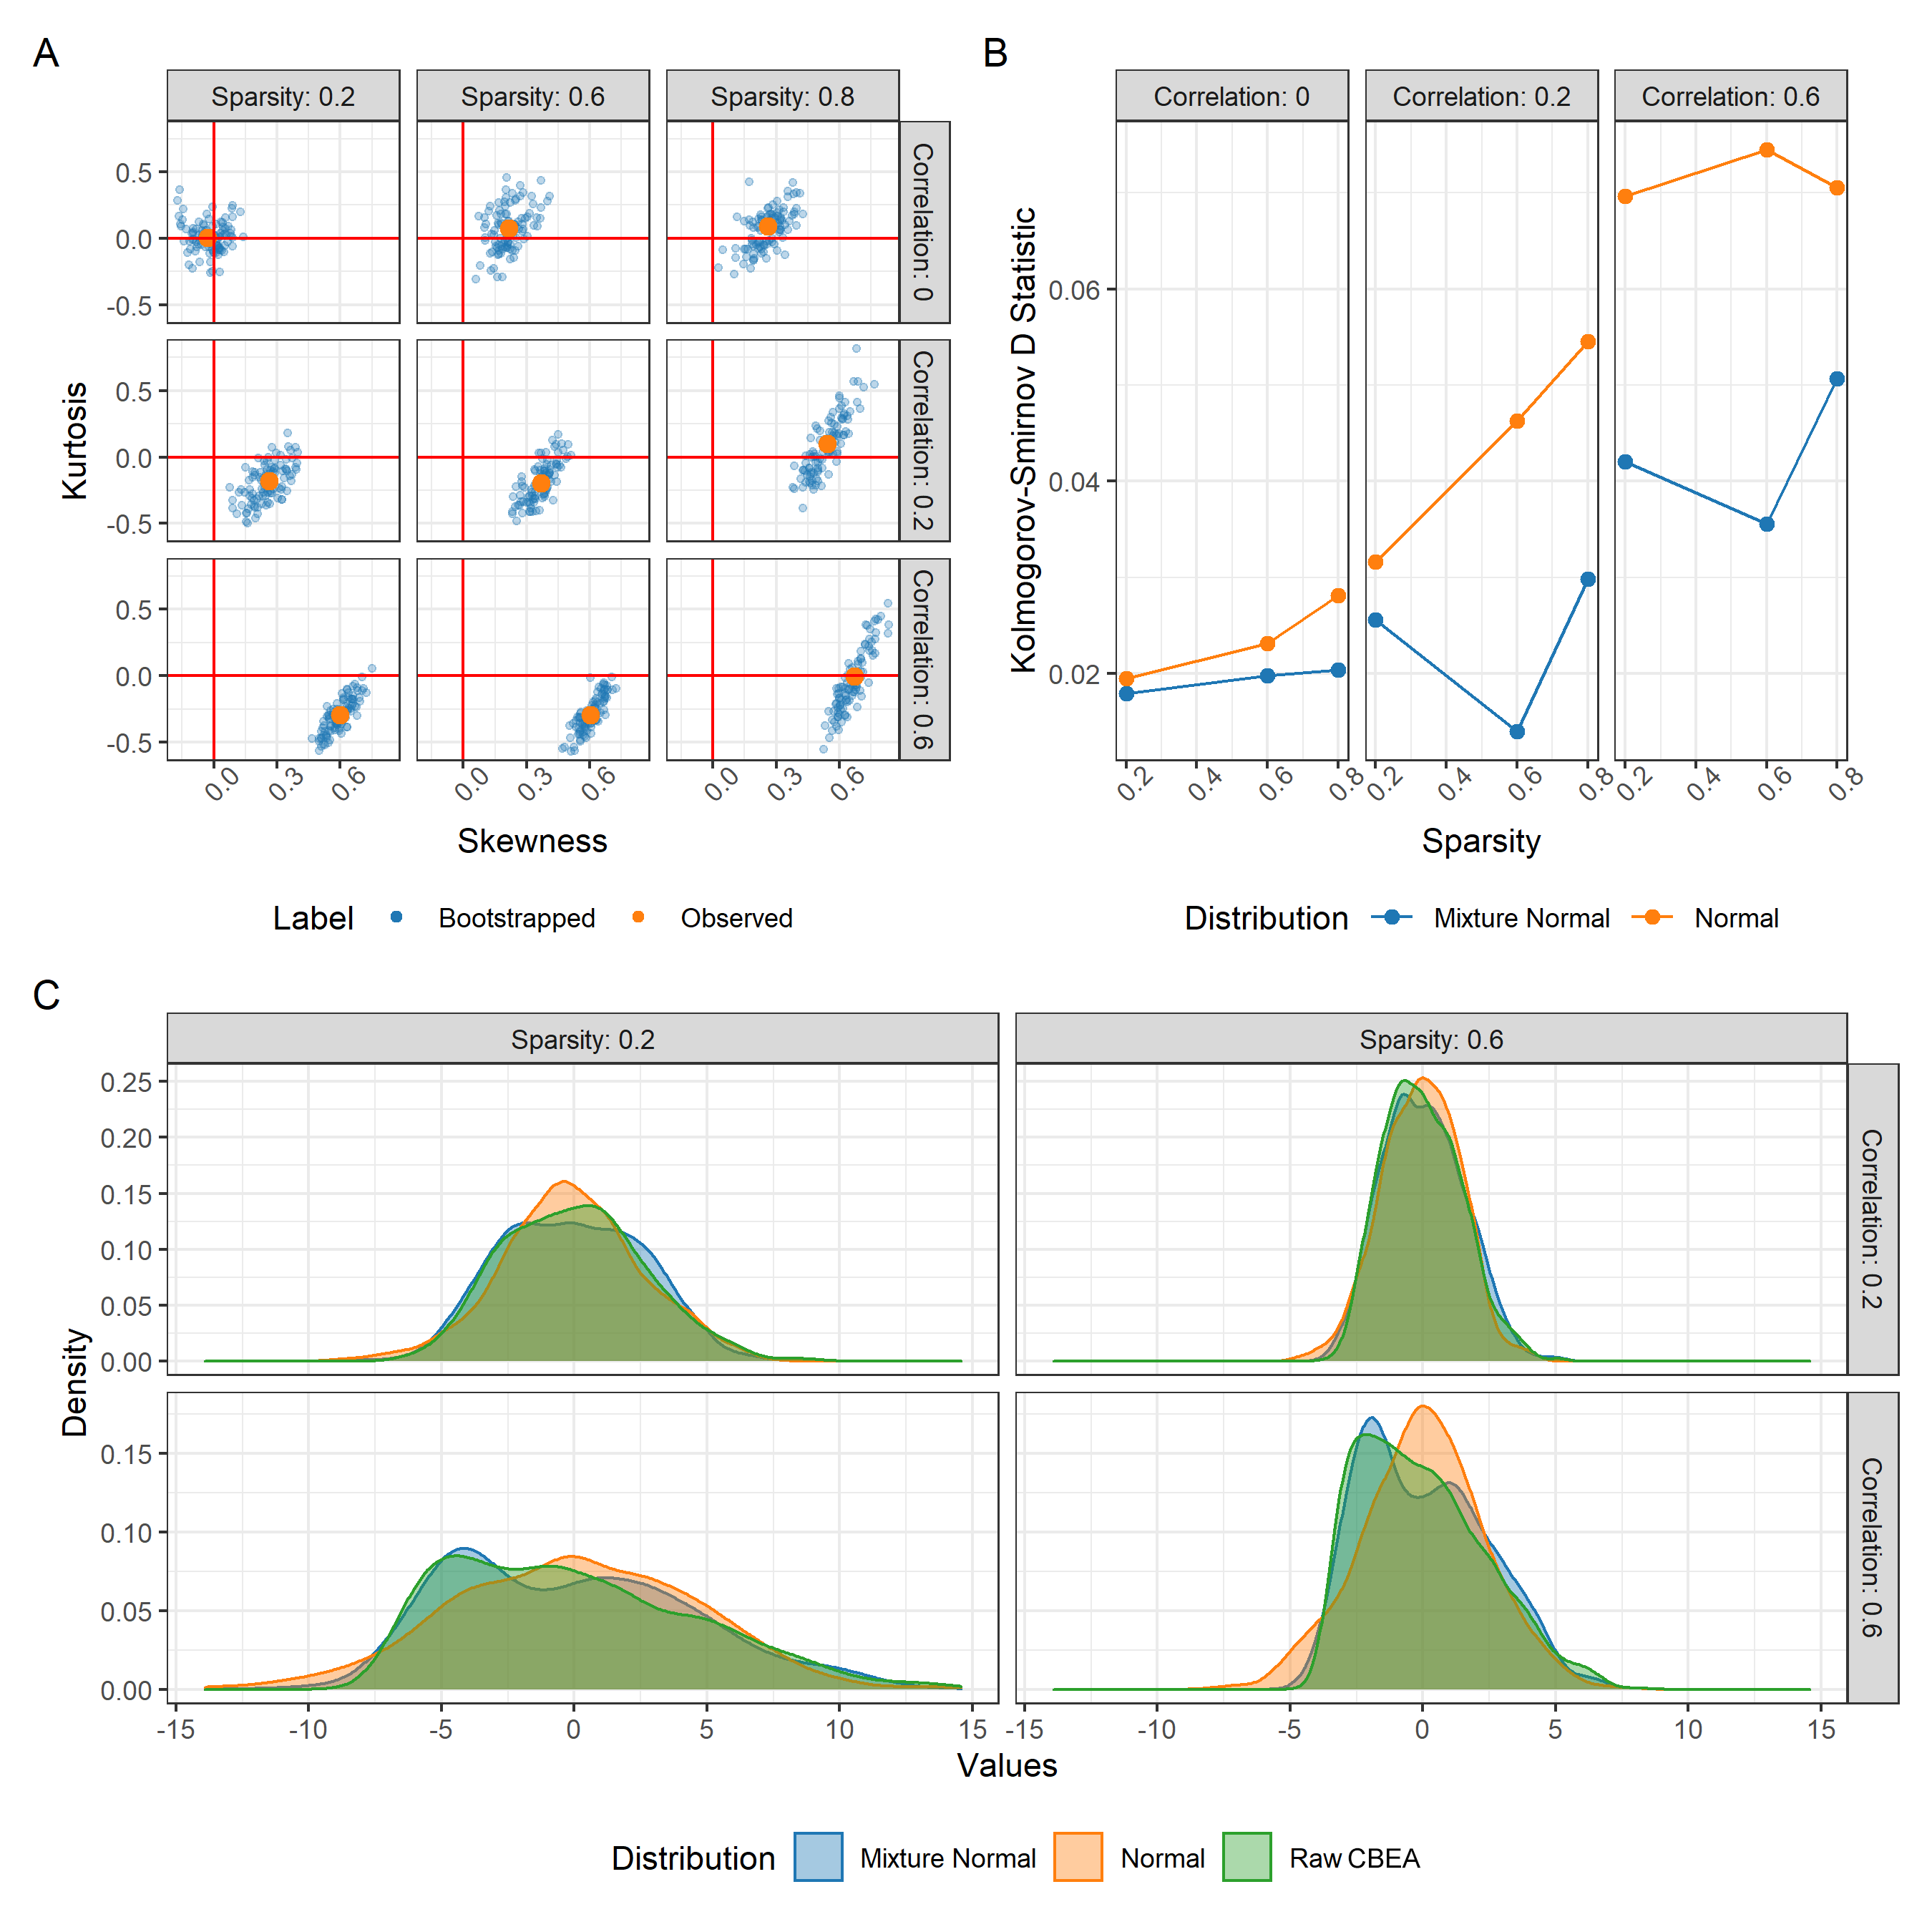
\includegraphics[width=\linewidth]{figures/ch3_f1.png}
    \caption[Properties of the null distribution of CBEA under the global null simulations]{Properties of the null distribution of CBEA under the global null simulations. Panel \textbf{(B)} presents kurtosis and skewness of CBEA scores while panel \textbf{(A)} presents the goodness of fit (as Kolmogorov-Smirnov D statistic) for mixture normal and normal distributions. Panel \textbf{(C)} is a density plot of the shape of the null distribution. Results indicated the necessity of estimating an empirical null and demonstrating that the mixture distribution was the better fit compared to the basic normal.}
    \label{fig:3.1}
\end{figure}

Additionally, the degree of kurtosis and skewness also suggests that the normal distribution itself might not be a good approximation of the null. To address this issue, we also evaluated a two-component normal mixture distribution. The goodness of fit of the mixture normal and the normal distribution using Kolmogorov-Smirnov (KS) test statistic computed on fitted normal and mixture normal distribution when fitted on CBEA scores in simulation scenarios under the global null is shown in Fig~\ref{fig:3.1}B. We can see that the mixture normal distribution is a better fit (lower KS scores) than the normal distribution across both sparsity and correlation settings. 

We performed our empirical null estimation by fitting our distribution of choice and computing relevant parameters on raw CBEA scores on taxa-permuted data (equivalent to gene permutation in the gene expression literature). As such, the null distribution is characterized by scores computed on sets of equal size with randomly drawn taxa. 

\subsubsection{Variance inflation due to inter-taxa correlation}  
When taxa within a set are highly correlated, the variance of the sample mean of taxon-wise statistics is inflated. Without loss of generalizability, for a set of taxa with taxon-specific statistics $x_1, \dots, x_p$ we have the variance of the mean $\bar{x}$ to be:  
\begin{equation} \label{vareq:1}
    Var(\bar{x}) = \frac{1}{m^2}\left(\sum_{i = 1}(\sigma_i^2) + \sum_{i < j}\rho_{ij}\sigma_i\sigma_j\right)
\end{equation}
where $\sigma_i$ is the standard deviation of taxon $i$ and $\rho_{ij}$ is the correlation between $i$ and $j$. The second term of (\ref{vareq:1}) is the correlation dependent variance component, which goes to 0 if there is no correlation. The CBEA statistic follows a similar pattern. Since the geometric mean of a set of variables is equivalent to the exponential of the arithmetic mean of their logarithms, we can re-write CBEA score for a set $k$ with size $K$ as follows:  
\begin{equation}\label{vareq:2}
    M_{i,k} = \sqrt{\frac{K(p - K)}{K + (p - K)}} \left( \overbar{\log{X_{i,j|j \in K}}} - \overbar{\log{X_{i,j|j \notin K}}} \right)   
\end{equation}
where $p$ is the overall number of taxa, $j$ is the index of a taxa and $K$ is the set of indices of taxa in set $k$. The CBEA statistic then looks similar to a t-statistic for difference in means of log-transformed proportions. As such, the pooled variance of CBEA is dependent on the variance inflation of both mean components $\overbar{\log{X_{i,j|j \in K}}}$ and $\overbar{\log{X_{i,j|j \notin K}}}$. The result of this variance inflation is inflated type I error since highly correlated sets are also detected as significantly enriched. 

However, as Wu et al. \cite{wu2012camera} showed, performing column permutation to estimate the null distribution of a competitive test statistic doesn't allow for adequate capture of this variance inflation factor since the permutation procedure disrupts the natural correlation structure of the original variables. It is important to address this problem since there is strong inter-taxa correlation within the microbiome \cite{kurtz2015sparse}. Our strategy for addressing this issue is to use the location (or mean) estimate from the column permuted raw score matrix with the spread (or variance) estimate taken from the original un-permuted scores. This still allows us to leverage the null distribution generated via column permutation while using the proper variance estimate taken from scores where the correlation structure has not been disrupted. As such, this procedure assumes that the variance of the test statistic under the alternate hypothesis is the same as that of the null. Details of the computational implementation to this estimation process can be found in the \nameref{appC_note1}.   

However, set-based analysis is an exploratory approach that can help generate functionally informative hypotheses, and as such users might not want strict type I error control in favor of higher power. This is especially true for competitive hypotheses, where its stricter formulation compared to the self-contained approach implies that the test naturally has lower power \cite{goeman2007analyzing, ackermann2009general}. Furthermore, sets that are highly correlated compared to background can be biologically relevant. Therefore, CBEA provides an option for users to specify whether correlation adjustment is desired. 

\section{Evaluation} \label{ch3_evaluation}
We based our evaluation strategy on gene set testing benchmarking standards set by Geistlinger et al. \cite{geistlinger2021gold} and utilized the same approaches whenever possible. All data sets are obtained from either the \texttt{curatedMetagenomicData} \cite{pasolli2017accessible} and \texttt{HMP16SData} \cite{schiffer2019hmp16sdata} R packages (2020-10-02 snapshot), or downloaded from the Qiita platform \cite{gonzalez2018qiita}. All code and data sets used for evaluation of this method is publicly available and can be found on GitHub (\url{www.github.com/qpmnguyen/CBEA_analysis}). Additional packages used to support this analysis includes: \texttt{tidyverse} \cite{wickham2019welcome}, \texttt{pROC} \cite{robin2011proc}, \texttt{phyloseq} \cite{mcmurdie2014waste}, \texttt{mia} \cite{ernst2021mia}, \texttt{targets} \cite{landau2021targets}.   

\subsection{Statistical significance}
We evaluate the inference procedure of CBEA compared to alternate methods using two approaches: randomly sampled taxa sets and sample label permutation. These analyses were performed on the 16S rRNA gene sequencing of the oral microbiome from the Human Microbiome Project \cite{consortium2012structure, proctor2019integrative}. This data set contains 369 samples split into two subsites: supragingival and subgingival. We processed this data set by removing all samples with total read counts less than 1000 and OTUs whose presence (at least 1 count) is in 10\% of samples or less.  

\subsubsection{Sample-level inference} 
Due to CBEA's self-contained null hypothesis, we can perform inference at the sample level for the enrichment of a set. We evaluated this application by generating one random taxon-set of different sizes $S \in \{20, 50, 100, 150, 200\}$ across 500 iterations. Random sets can act as our estimate for type I error since this matches the CBEA null hypothesis stated in \nameref{ch3_methods}, where we expect within each sample, sets of randomly drawn taxa should not be significantly enriched compared to the remainder background taxa. For this evaluation, we estimated type I error as the fraction of samples where our random set is detected as significant at a p-value threshold of 0.05 with confidence bands computed from the standard error across all iterations.  Additionally, this analysis also tests whether CBEA is sensitive to different set sizes.  

\subsubsection{Population-level inference} 
We can perform enrichment testing at the population level by generating corresponding sample level CBEA scores and performing a two-sample test such as Welch's t-test. In order to evaluate CBEA under this context, we generated CBEA scores of sets representing genus-level annotation in above gingival data set \cite{consortium2012structure, proctor2019integrative} and applied a t-test to test for enrichment (similar to GSVA \cite{hanzelmann2013gsva}) across a randomly generated variable indicating case/control status (repeated 500 times). Type I error is estimated as the fraction of sets per iteration found to be significantly enriched with confidence bands computed from the standard error across all iterations. In addition, we also performed a random set analysis assessment, where we generated 100 sets of different set sizes $S \in \{20, 50, 100, 150, 200\}$ and evaluated the fraction of genera that were found to be differentially abundant across the original labels (supragingival versus subgingival subsite). 95\% confidence intervals were computed using the Agresti-Couli approach \cite{agresti1998approximate}.  

\subsection{Phenotype relevance}
We want to evaluate whether sets found to be significantly enriched by CBEA are relevant to the research question. To perform this assessment, we relied on the gingival data set mentioned above \cite{consortium2012structure, proctor2019integrative}. This data set was chosen because its clear biological interpretation can serve as the ground truth. Specifically, we expect aerobic microbes to be enriched in the supragingival subsite where the biofilm is exposed to the open air, while conversely anaerobic microbes thrive in the subgingival site \cite{thurnheer2016microbial}. Genus-level annotations for microbial metabolism from Beghini et al. \cite{beghini2019tobacco} were obtained from the GitHub repository associated with Calagaro et al. \cite{matteocalgaro2020mcalgaro93}. For sample-level inference, we assessed power as the fraction of supragingival samples where aerobic microbes are significantly enriched. For population-level inference, power is the fraction of sets representing genus level taxonomic assignments that were significant across subsite labels.  

In addition to statistical power, we also assessed phenotype relevance through evaluating whether highly ranked sets based on CBEA scores are more likely to be enriched according to the ground truth. This is represented by the area under the receiving operator curve (AUROC/AUC) scores computed on CBEA scores against true labels (similar approach was used to evaluate VAM \cite{frost2020varianceadjusted}). DeLong 95\% confidence intervals for AUROC \cite{delong1988comparing} were obtained for each estimate. 

\subsection{Disease Prediction}
CBEA scores can also be used for downstream analyses such as disease prediction tasks. We utilized two data sets for this evaluation: 

\begin{enumerate}
\item Whole genome sequencing of stool samples from inflammatory bowel disease (IBD) patients in the MetaHIT consortium \cite{nielsen2014identification}. This data set contains 396 samples from a cohort of European adults, where 195 adults were classified as having IBD (which includes patients diagnosed with either ulcerative colitis or Crohn's disease). We processed this data by removing all samples with less than 1,000 total read counts as well as any OTU that was present (with non-zero proportions) in 10\% of the samples or less. Prior to model fitting, we back-transformed relative abundances into count data (to align the format with our 16S rRNA gene sequencing data set) using the provided total number of reads aligned to MetaPhlan marker genes (per sample).   

\item 16S rRNA gene sequencing of stool samples from IBD patients in the RISK cohort \cite{gevers2014treatmentnaive}. This data set contains 16S rRNA gene sequencing samples from a cohort of pediatric patients (ages $<$ 17) from the RISK cohort enrolled in the United States and Canada. Of the 671 samples obtained, 500 samples belong to patients with IBD. We processed this data set by removing all samples with less than 1,000 total read counts as well as any OTU that was present (at least 1 count) in 10\% of the samples or less.   
\end{enumerate}

We evaluate disease prediction performance by fitting a random forest model \cite{breiman2001random} using as inputs CBEA scores to classify samples of patients with IBD and healthy controls. Random forest was chosen as a baseline learner due to its flexibility as an out-of-the-box model that is easy to fit. In this instance we evaluated predictive performance of a default random forest model (without hyperparameter tuning) AUROC after 10-fold cross validation. Additionally, we utilized SMOTE to correct for class imbalances \cite{chawla2002smote}. Implementation was done using the \texttt{tidymodels} suite of packages \cite{kuhn2020tidymodels}.   

\subsection{Comparison Methods} 
We benchmarked the statistical properties of CBEA against existing baseline approaches. For sample-level inference analyses, utilized the Wilcoxon rank-sum test, which non-parametrically tests the difference in mean counts between taxa from a pre-defined set and its remainder similar to CBEA. For assessments at the population level, we compared CBEA against performing a standard test for differential abundance with set-level features generated via element-wise summations instead. We chose DESeq2 \cite{love2014moderated} and corncob \cite{martin2020modeling} because they represent both methods extrapolated from RNA-seq \cite{mcmurdie2014waste} and those developed specifically for microbiome data.   

Since disease prediction models and rankings-based phenotype relevance analyses seek to evaluate the informativeness of CBEA scores instead of relying on computing p-values, we compared performance against other single sample based approaches from the gene set testing literature, specifically ssGSEA \cite{barbie2009systematic} and GSVA \cite{hanzelmann2013gsva}. Additionally, for evaluating prediction, we also compared performance against a standard analysis plan where inputs are count-aggregated sets with the centered log-ratio (CLR) transformation. 

\section{Results}
In this section, we present results for evaluating statistical significance, phenotype relevance, and predictive performance. In addition to real data, we also evaluated models based on parametric simulations, where results can be found in the Supplemental Materials.   

\subsection{Statistical Significance}
\subsubsection{Inference at the sample level}
CBEA provides significance testing at the sample level through a self-contained competitive null hypothesis. Generating random sets approximate the global null setting where within each sample, sets generated by randomly sampling taxa should not be significantly more enriched than remainder taxa.   

\begin{figure}[!h]
    \centering
    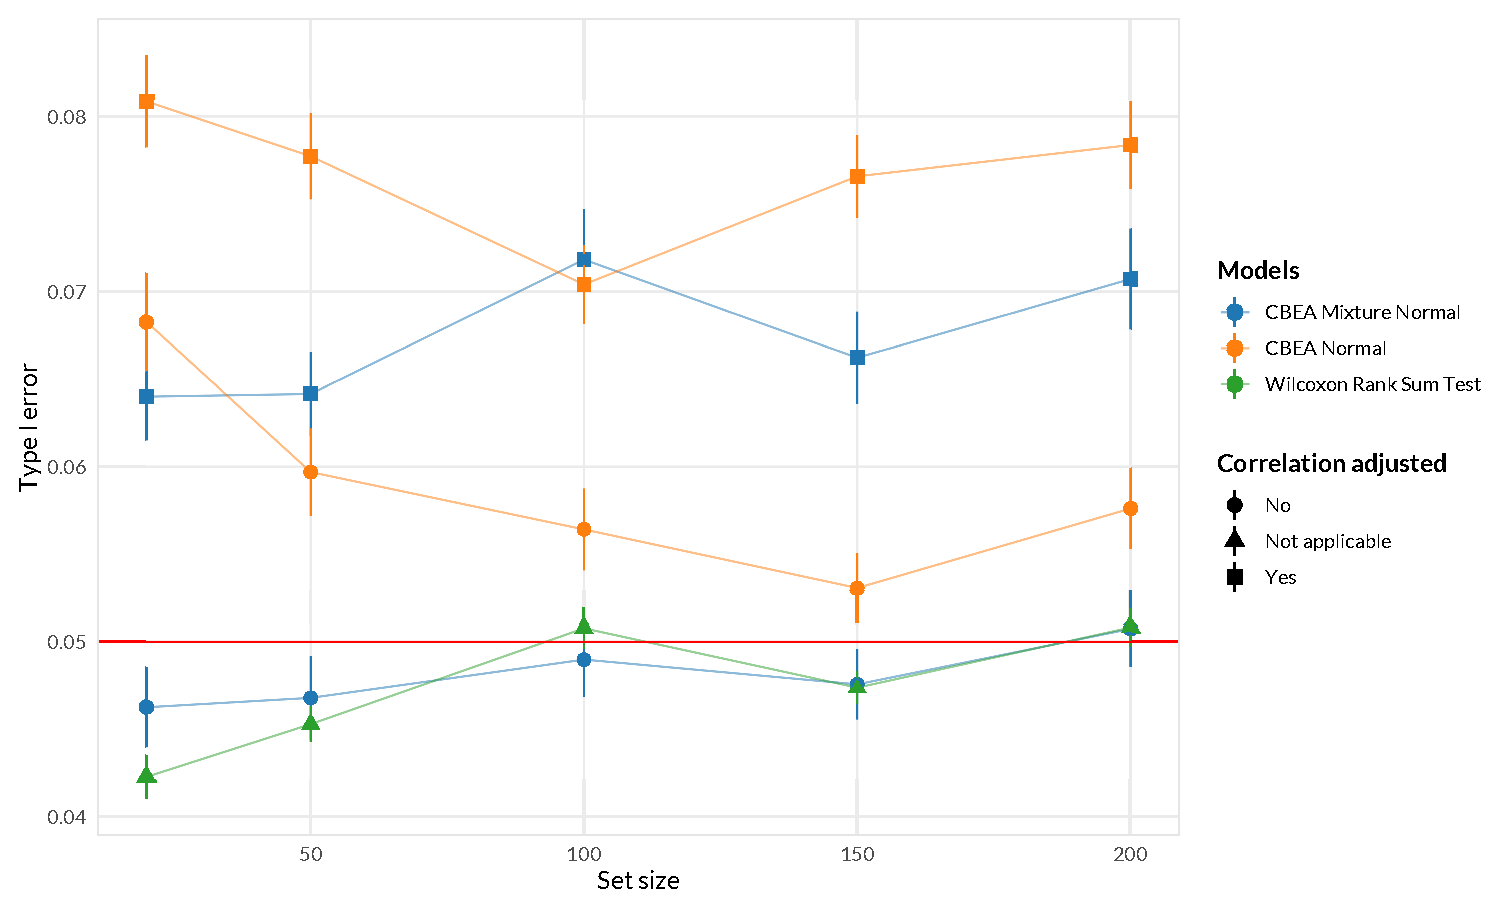
\includegraphics[width = \textwidth]{figures/ch3_f2.eps}
    \caption[Random taxa set analyses for inference at the sample level of CBEA under different parametric assumptions compared against a Wilcoxon rank-sum test]{Random taxa set analyses for inference at the sample level of CBEA under different parametric assumptions compared against a Wilcoxon rank-sum test. Type I error (\emph{y}-axis) was evaluated by generating random sets of different sizes (\emph{x}-axis) (500 replications per size) and computing the fraction of samples where the set was found to be significantly enriched at $\alpha = 0.05$. Error bars represent the mean type I error $\pm$ sample standard error computed across 500 replications of the experiment. Only the unadjusted CBEA with the mixture normal distribution and the Wilcoxon rank sum test were able to control for type I error at 0.05. All approaches are invariant to set sizes.} 
    \label{fig:3.2}
\end{figure}

Fig~\ref{fig:3.2} demonstrates type I error of sample-level inference evaluated using the random set approach. The Wilcoxon rank sum test and unadjusted CBEA under mixture normal assumption demonstrated good type I error control at the appropriate $\alpha$ level. This fits with our expectations since the mixture normal distribution has a much better fit than the normal distribution especially at the tails of the empirical distribution (Fig~\ref{fig:3.1}). However, other variants of CBEA demonstrated inflated type I error, especially correlation adjusted variants compared to their unadjusted counter parts. Encouragingly, all methods demonstrate consistent performance across all set sizes, with a slight increase in type I error at the highest levels.   

Interestingly, simulation results (Fig~\ref{fig:c1}) showed an opposite pattern. Adjusted approaches were good at controlling for type I error, especially under the low inter-taxa correlation values within the set (similar to generating random sets where the natural correlation structure is disrupted). In these simulations, unadjusted approaches and the Wilcoxon rank sum test had significant type I error inflation with increasing correlation. All approaches seems to be invariant to the level of data sparsity.  

\subsubsection{Inference at the population level}

Similar to other single sample approaches to gene set testing such as GSVA \cite{hanzelmann2013gsva}, we can perform inference at the population level by utilizing a two-sample difference in means test. Here, we evaluate using CBEA scores generated under different settings with Welch's t-test in a supervised manner to assess whether a set is enriched across case/control status. 

\begin{figure}[!h]
    \centering
    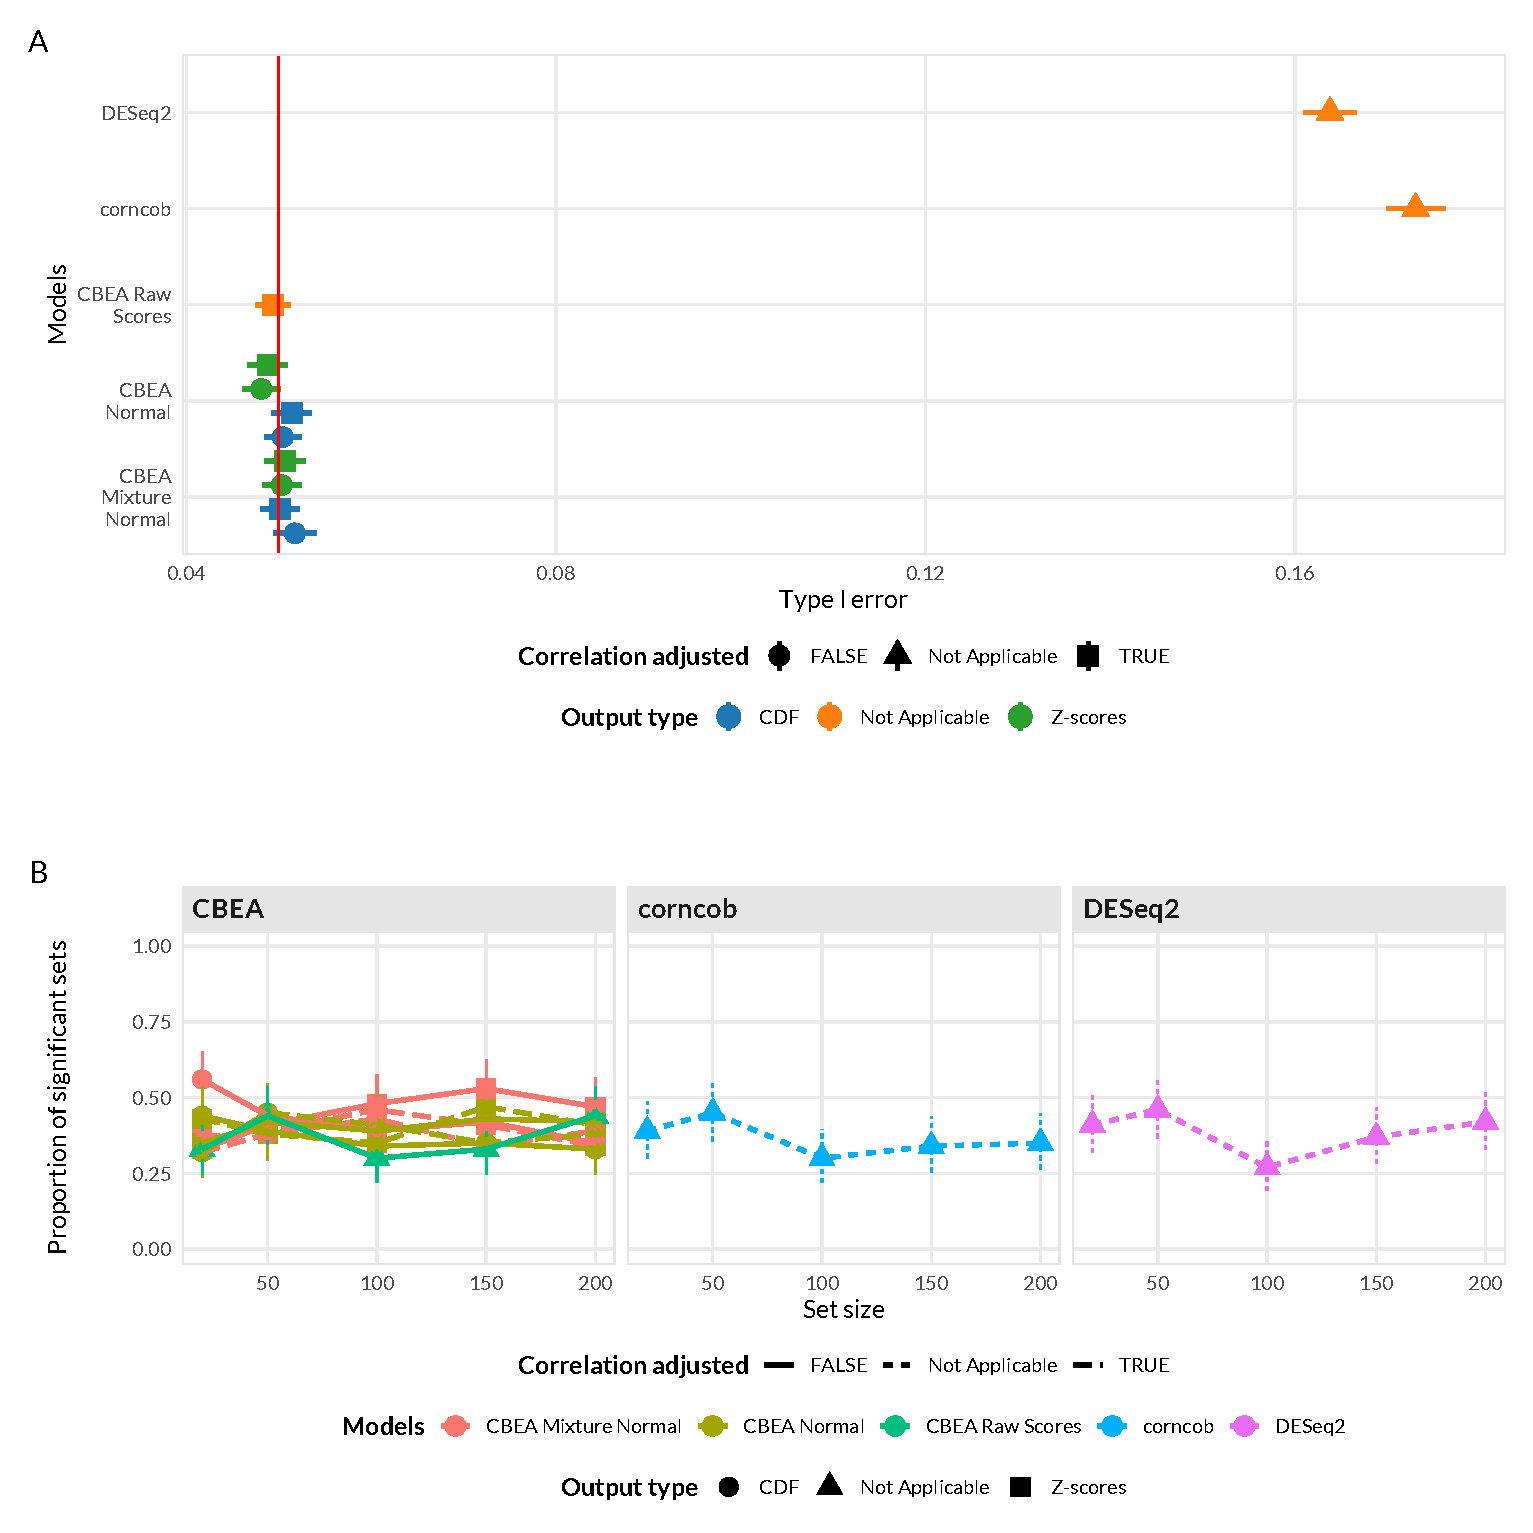
\includegraphics[width = \textwidth]{figures/ch3_f3.eps}
    \caption[Random sample label (\textbf{A}) and random set (\textbf{B}) analyses for population level inference]{Random sample label (\textbf{A}) and random set (\textbf{B}) analyses for population level inference. (\textbf{A}) Type I error (\emph{x}-axis) was estimated as the overall fraction of sets found to be enriched $\alpha = 0.05$ using randomly generated sample labels (500 permutations).  Error bars represent the mean type I error $\pm$ sample standard error. (\textbf{B}) Proportion of significant sets (\emph{y}-axis) using 100 randomly generated sets of different set sizes (\emph{x}-axis). Confidence intervals computed using Agresti-Couli method for binomial proportions. For sample label permutation (\textbf{A}), all CBEA approaches were able to control for type I error but not for corncob and DESeq2. For random set analyses (\textbf{B}), all approaches demonstrate similar rate of accepting significant sets and were invariant to overall set size.}  
    \label{fig:3.3}
\end{figure}

Fig~\ref{fig:3.3} shows results for this scenario using both random sample label and random set evaluations. The random sample label approach (Fig~\ref{fig:3.3}A) provides a controlled setting where we can estimate type I error rate controlled at $\alpha = 0.05$. Across all replications, CBEA methods were able to control for type I error at the nominal threshold of 0.05, with CBEA raw scores being the most performant. Neither output types, correlation adjustment, nor distributional assumption improved performance values. Surprisingly, DESeq2 and corncob both exhibit significantly inflated type I error. 

We also assessed the impact of set-size on the inference procedure by testing for enrichment using the original sample labels but with randomly sampled sets of different sizes (Fig~\ref{fig:3.3}B). Overall we observed very similar values across CBEA as well as corncob and DESeq2, suggesting that no individual method is systematically identifying too many significant sets. Additionally, similar to analogous analyses at the sample level, no approach was significantly sensitive to changes in set sizes.  

\subsection{Phenotype Relevance} 
\subsubsection{Inference at the sample level}
\begin{figure}[!h]
    \centering
    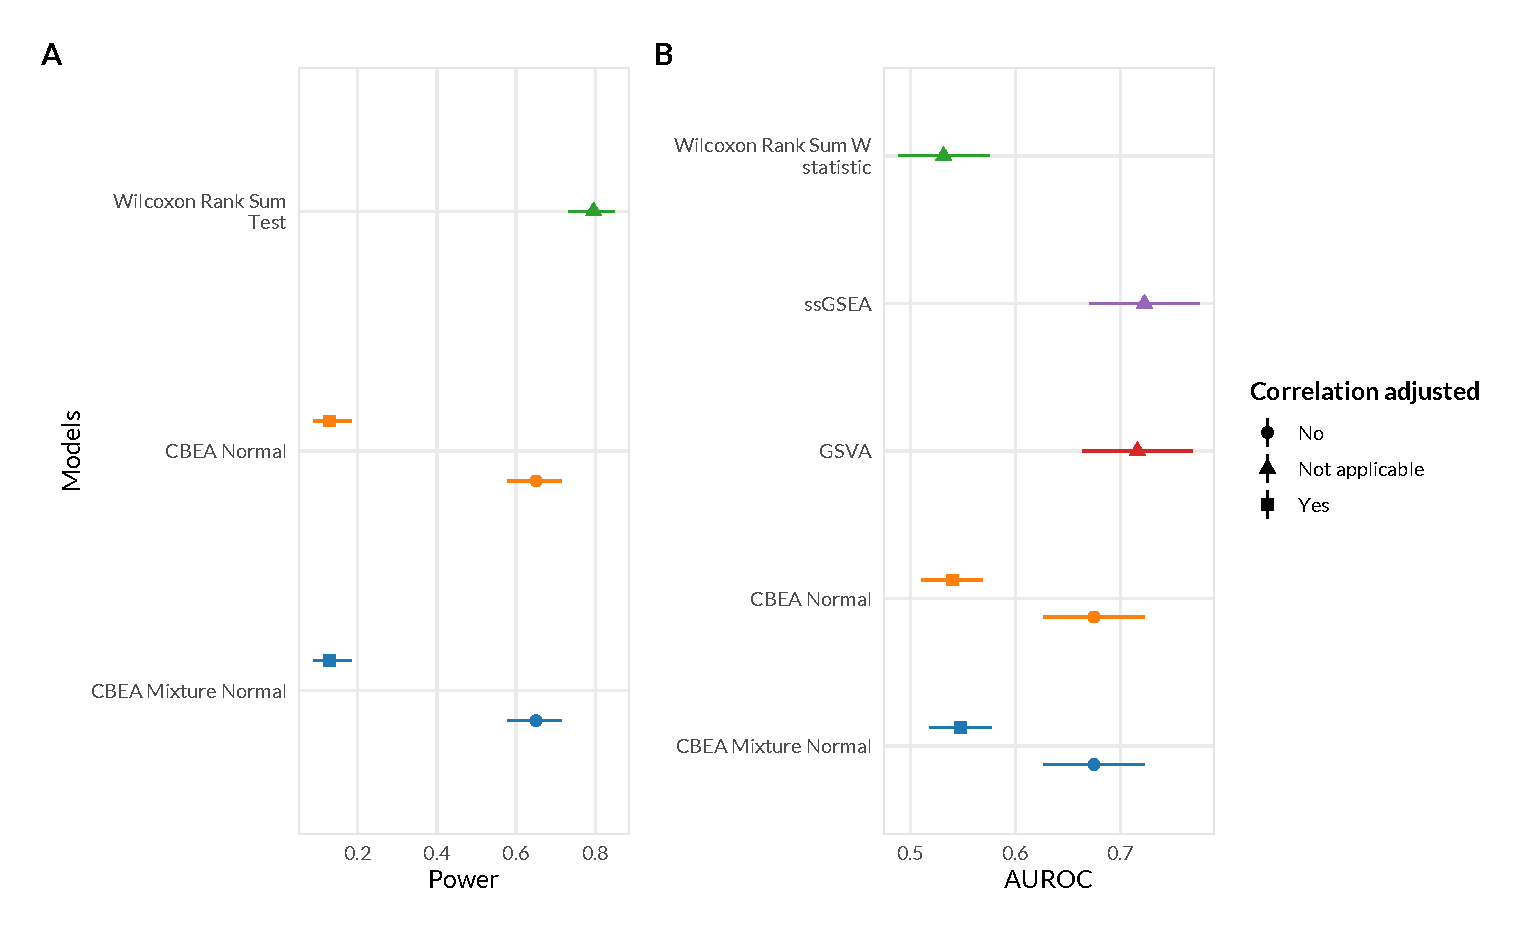
\includegraphics[width = \textwidth]{figures/ch3_f4.eps}
    \caption[Statistical power (\textbf{A}) and score rankings (\textbf{B}) to assess phenotype relevance]{Statistical power (\textbf{A}) and score rankings (\textbf{B}) to assess phenotype relevance. (\textbf{A}) Power (\emph{x}-axis) was estimated as the overall fraction of aerobic microbes found to be enriched in supragingival samples at $\alpha = 0.05$. 95\% confidence intervals were computed using the Agresti-Couli approach for binomial proportions. (\textbf{B}) Score rankings were evaluated by comparing computed scores against true values using AUROC (\emph{x}-axis). DeLong 95 \% confidence intervals for AUROC were computed.} 
    \label{fig:3.4}
\end{figure}

In Fig~\ref{fig:3.4}, we evaluate whether sets found to be significant by CBEA are relevant to the phenotype of interest. We leveraged the gingival data set as stated in \nameref{ch3_evaluation} section where we know beforehand that aerobic microbes are more likely to be enriched in supragingival subsite samples and vice versa. 

We estimated statistical power using this data set as the fraction of supragingival samples where the set representing aerobic microbes were significantly enriched. We observed that adjusted CBEA approaches demonstrate much lower power compared to the Wilcoxon rank-sum test and unadjusted variants. This is surprising given the fact that in statistical significance analyses, the adjusted CBEA approach provides inflated type I error, especially if the normal distribution assumption was chosen, which indicates a mismatch in estimating the null distribution since a high type I error did not result in increased power. 

We also evaluated phenotype relevance by assessing whether enriched sets according to ground truth are preferentially ranked higher using assigned continuous scores (instead of performing a hypothesis test). This aspect is captured through computing AUROC values comparing computed enrichment scores and true labels. Consistent with the previous type I error evaluation, adjusting for correlation did not improve performance, where obtained AUROC were around 0.5 and at the same level as the benchmark Wilcoxon rank sum statistic. Unadjusted methods were much better at ranking true enriched sets, however the mean AUROC values are lower than alternate single sample enrichment methods (GSVA \cite{hanzelmann2013gsva} and ssGSEA \cite{barbie2009systematic}) even though this difference is not significant due to overlapping confidence intervals.  

The above results were replicated in simulation studies where we observed that adjusted approaches were very conservative and demonstrated significantly lower power (Fig~\ref{fig:c3}) with increasing correlation even at the highest evaluated effect sizes. When assessing score rankings, the performance of CBEA was closer to ssGSEA and GSVA compared to real data evaluations, however all single sample approaches were much better than using the W statistic from the Wilcoxon Rank Sum test.   

\subsubsection{Inference at the population level}
\begin{figure}[!h]
    \centering
    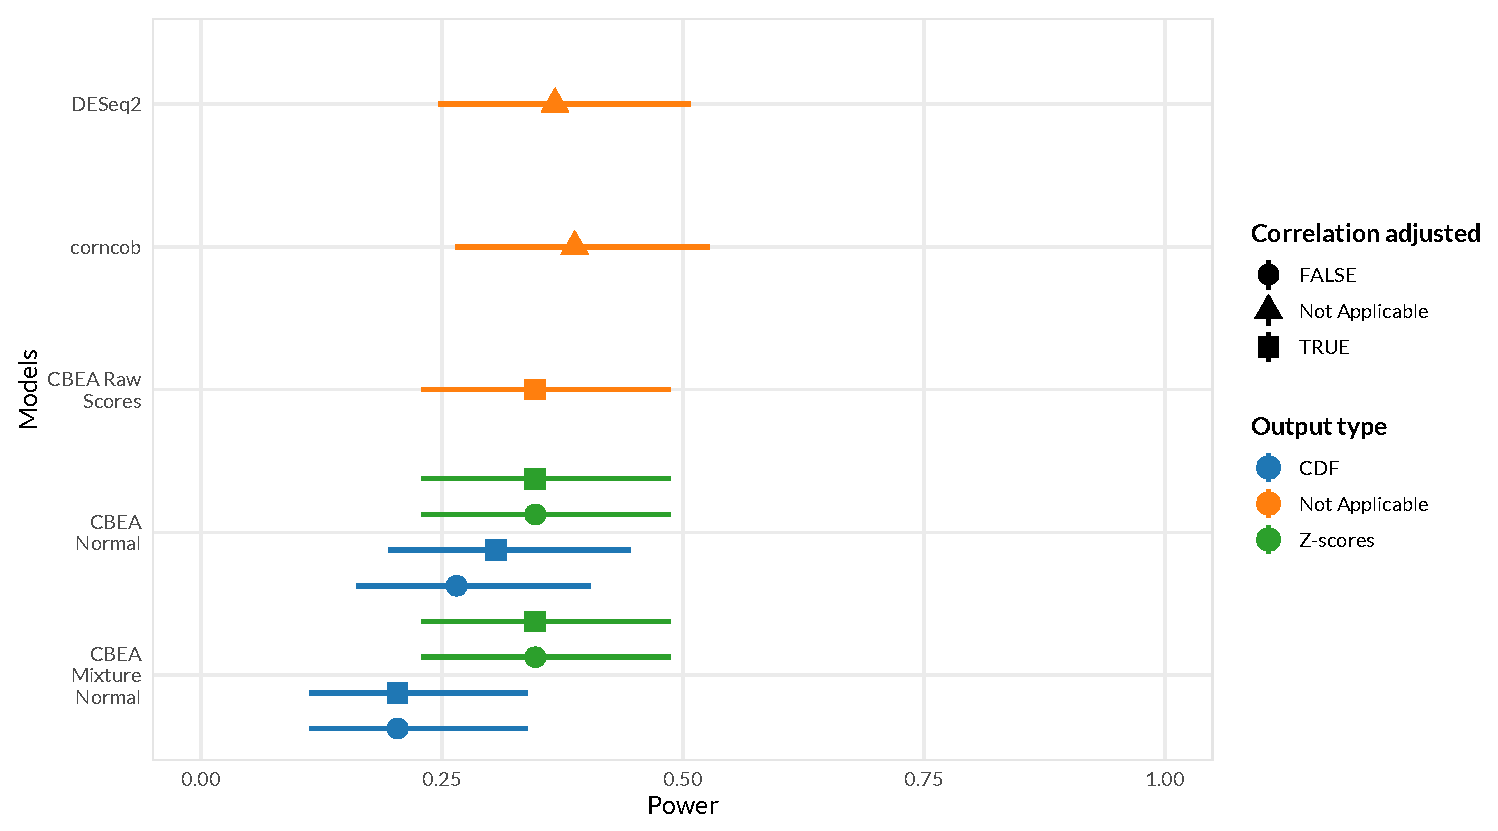
\includegraphics[width = \textwidth]{figures/ch3_f5.eps}
    \caption[Statistical power to assess phenotype relevance of inference tasks at the population level]{Statistical power to assess phenotype relevance of inference tasks at the population level. Power (\emph{x}-axis) was estimated as the overall fraction of sets representing genera that are aerobic or anaerobic microbes found to be differentially enriched across sample type (supragingival or subgingival). 95\% confidence intervals were computed using the Agresti-Couli approach for binomial proportions.}  
    \label{fig:3.5}
\end{figure}

We also assessed statistical power for population level inference scenarios using a similar approach. Here, enrichment scores for sets representing all identified genera were computed, and power was estimated as the fraction of sets found to be differentially enriched across sample site labels (supragingival or subgingival). We compared these results against performing a differential abundance test of genus level features generated via sum-based approaches. Results are shown in Fig~\ref{fig:3.5}. Some CBEA variants, such as CDF outputs for the mixture normal distributional assumption, did not correctly detect as many significant sets as DESeq2 or corncob despite very close performance values. Using raw CBEA scores was best approach, however it did not exceed values obtained from DESeq2 and corncob. 

\subsection{Disease Prediction}   
Since CBEA can generate informative scores that can discriminate between samples with inflated counts for a set (Fig~\ref{fig:3.4}), we wanted to assess whether they can also act as useful inputs to predictive models. In this section we assessed the predictive performance of a standard baseline random forest model \cite{breiman2001random} with different single sample enrichment scoring methods as inputs (CBEA, ssGSEA, and GSVA). Additionally, we also compared predictive performance of using these scores against the a standard approach of using the centered log ratio transformation (CLR) on taxon sets aggregated via abundance summations.     

We fit our model to two data sets with a similar disease classification task of discriminating patients who were diagnosed with IBD (includes both Crohn's disease and ulcerative colitis) using only microbiome taxonomic composition. The two data sets represent different microbiome sequencing aprpaoches: the Gevers et al. \cite{gevers2014treatmentnaive} data set uses 16S rRNA gene sequencing, while the Nielsen et al \cite{nielsen2014identification} data set uses whole genome shotgun sequencing. 

\begin{figure}[!h]
    \centering
    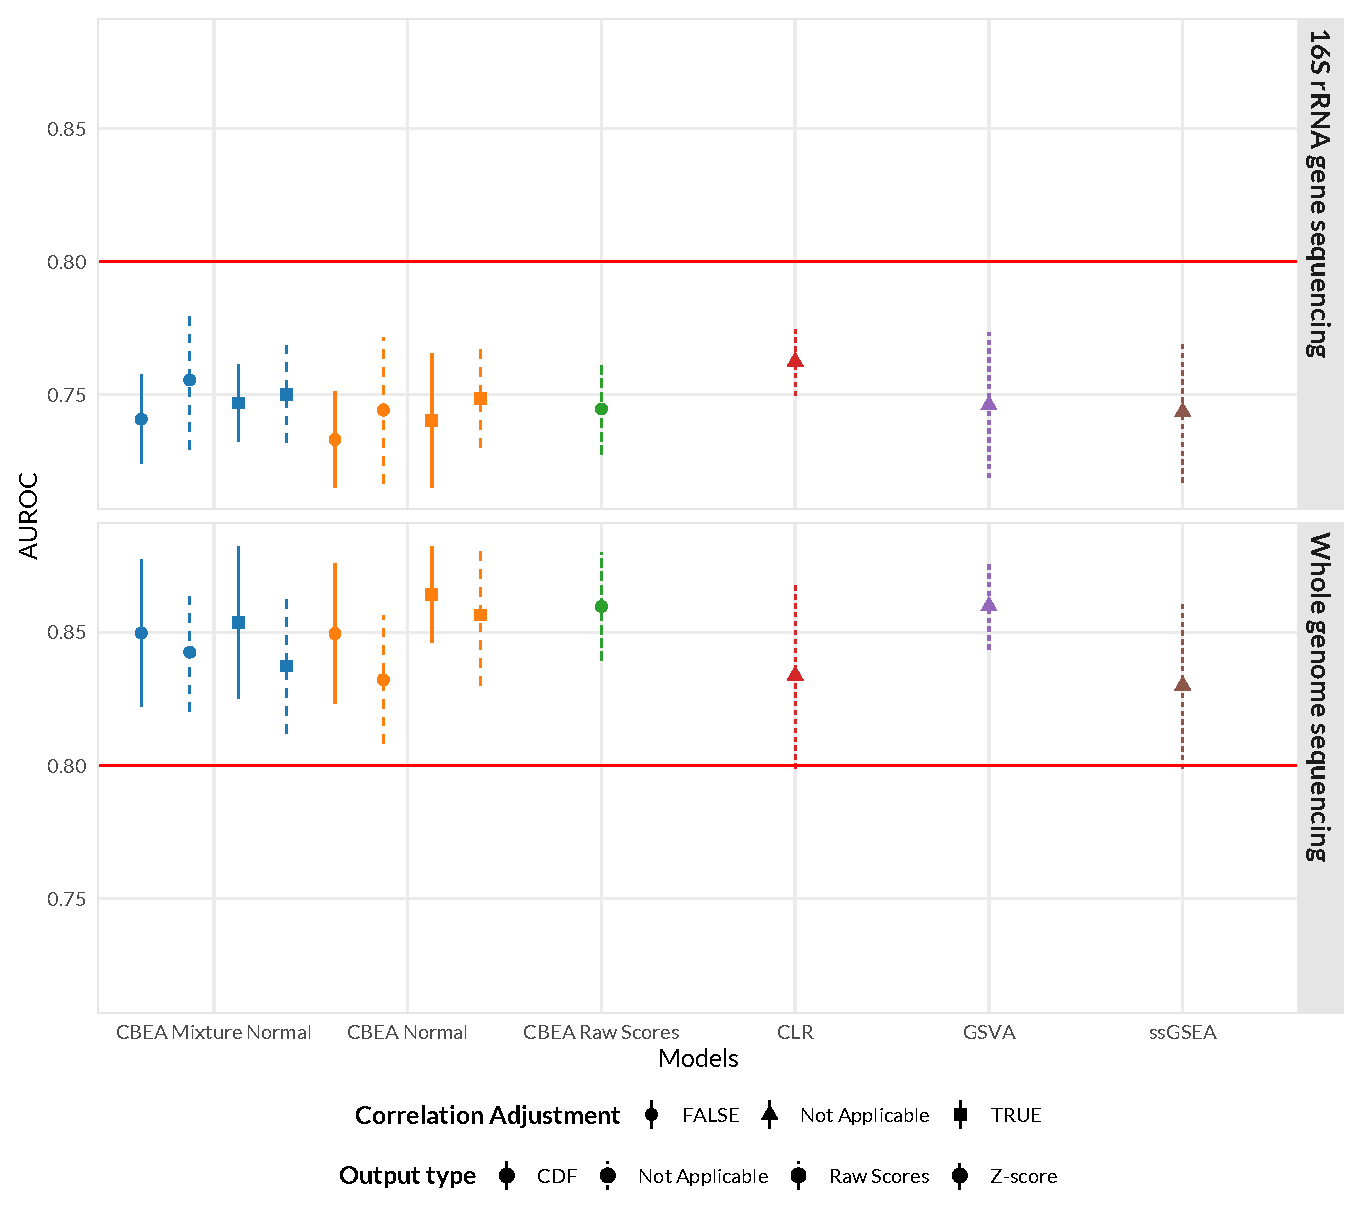
\includegraphics[width = \linewidth]{figures/ch3_f6.eps}
    \caption[Predictive performance of a naive random forest model trained on CBEA, ssGSEA, GSVA generated scores as well as the standard CLR approach on predicting patients with inflammatory bowel disease versus controls using genus level taxonomic profiles]{Predictive performance of a naive random forest model trained on CBEA, ssGSEA, GSVA generated scores as well as the standard CLR approach on predicting patients with inflammatory bowel disease versus controls using genus level taxonomic profiles. Data sets used span both 16S rRNA gene sequencing (Gevers et al. \cite{gevers2014treatmentnaive}) and whole-genome shotgun sequencing (Nielsen et al. \cite{nielsen2014identification}). CBEA performs better than GSVA and ssGSEA but not as well as CLR, with the exception of the whole genome sequencing data set.}
    \label{fig:3.6}
\end{figure}

Fig~\ref{fig:3.6} illustrates the performance of our model with AUROC as the evaluation criteria. In the 16S rRNA data set, the best performing CBEA variant (CDF values computed from an unadjusted mixture normal distribution) outperforms both GSVA and ssGSEA but not the standard CLR approach. Interestingly, in the whole genome sequencing data set, CBEA outperforms CLR, but was similar in performance to GSVA. However, due to large confidence intervals, no method significantly out-performed other evaluated approaches. As such, these results indicate that, for a given pre-determined collection of sets, CBEA generated scores are can be informative and provide competitive performance when acting as inputs to disease predictive models. Simulation studies (Fig~\ref{fig:c5}) showed similar results, however CBEA more consistently underperformed compared to CLR across all scenarios. Interestingly, the performance gap decreases with increasing sparsity levels and correlation. 

\section{Discussion}

\subsection{Inference with CBEA} 
CBEA is a microbiome-specific approach to generate sample specific enrichment scores for taxonomic sets defined \emph{a priori}. The formulation of CBEA as a comparison between taxa within the set and its complement corresponds to the competitive null hypothesis in the gene set testing literature \cite{tian2005discovering}. Since this null hypothesis is self-contained per sample, this allows users perform enrichment testing at the sample level. Additionally, in combination with a difference in means test, CBEA can also test for enrichment at the population level across case/control status similar to GSVA \cite{hanzelmann2013gsva}.  

For single-sample analyses, we demonstrated that the CBEA approach (unadjusted with mixture normal parametric assumption) was able to control for type I error at the nominal level of 0.05 under the global null (Fig~\ref{fig:3.2}) while also demonstrating adequate power (Fig~\ref{fig:3.4}). This performance is consistent across different set sizes as well as our prior distributional fit analyses (Fig~\ref{fig:3.1}), where the mixture normal displayed superior fit to the null distribution. Unfortunately, other variants of CBEA demonstrated neither good type I error control nor power. Interestingly, while the adjusted methods showed poor performance in real data evaluations (Fig~\ref{fig:3.2}), in simulation studies (Fig~\ref{fig:c1}, Fig~\ref{fig:c3}) these approaches were able to control for type I error well with the trade-off of much lower power. 
For the population-level inference task, CBEA also performed very well. Under the permutation global null, representing genera abundance using CBEA scores in combination with Welch's t-test controls for type I error at the correct $\alpha$ threshold while also keeping respectable power. Since the population level enrichment test is equivalent to a differential abundance test using set-based features, we compared the CBEA approach against using element-wise summations with corncob \cite{martin2020modeling} and DESeq2 \cite{love2014moderated} to test for set-level differential abundance. We chose DESeq2 because it is an older approach from the bulk RNA-seq literature that has strong support for usage in microbiome taxonomic data \cite{mcmurdie2014waste}. Alternately, corncob is a newer method developed specifically for microbiome taxonomic data sets, where taxonomic counts are modeled directly using a beta-binomial distribution instead of relying on normalization via size factor estimation. We observed that using this approach resulted in an inflated type I error compared to all variants of CBEA (Fig~\ref{fig:3.2}), yet did not improve power (Fig~\ref{fig:3.4}). Results for CBEA approaches were replicated in simulation analyses, however for corncob and DESeq2 we observed an opposite effect: in simulation experiments, both methods show good type I error control but low power (Fig~\ref{fig:c2}, Fig~\ref{fig:c4}).

We hypothesized that the discrepancy between simulation and real data evaluations could be due to differences in our assumptions regarding the data generating process that informed our simulation schema. For the non-zero component of each taxon, we sampled from the same negative binomial distribution where designated enriched taxa were generated with inflated means (but the same dispersion). These marginals were simulated to account for block exchangable correlation within the enriched set only. This might have affected our results in two ways. First, our simulation scenario ensures that all designated non-enriched taxa are identical to each other. This is not the case for real data, where our null scenario involves randomly sampled sets that might by chance all have taxa with inflated means compared to remainder taxa. This is represented in Fig~\ref{fig:c7}, where the distribution of type I error across 500 replications is right skewed for underperforming CBEA variants, indicating that these approaches are much more sensitive compared to the Wilcoxon rank sum test or unadjusted CBEA with mixture normal distribution. Second, as described in the \nameref{ch3_background} section, we did not consider taxon-specific biases that distort the observed relative abundance of taxa compared to true values \cite{mclaren2019consistent}. In the context of sum-based aggregations, the resulting bias of the aggregated taxon-set is dependent on the relative abundances of the contributing taxa (Appendix I in \cite{mclaren2019consistent}). Conceptually, this means that measurement error for a taxon-set is different across samples as relative abundance of contributing taxa changes, leading to issues when attempting to perform inference. As such, we expect methods like corncob or DESeq2 when performed on such sum aggregates in the presence of taxon-specific biases to have inflated type I error compared to our multiplication based approach. This also explains why conversely in simulation studies, where taxon-specific biases are absent, corncob and DESeq2 performed better. 
\subsection{Downstream analysis using predictive models}
The sample-level enrichment scores generated by the CBEA method can be used in downstream analyses such as disease prediction. We evaluated whether CBEA can be used to generate set-based features for disease prediction models. 
We fit a basic random forest model \cite{breiman2001random} to predict continuous and binary outcomes using CBEA generated scores as inputs. Similar to our inference analysis, we compared CBEA against both ssGSEA and GSVA. Additionally, we also evaluated CBEA with the approach where counts of a set were aggregated using sums and applied the centered log-ratio transformation (CLR). This is because CLR is considered standard practice in using microbiome variables as predictors for a model \cite{gloor2017microbiome}. Results showed that CBEA generate scores perform well across both real data and simulation scenarios. Since predictive models consider the effect of variables jointly (and in the case of random forest, consider interactions as well), good performance indicates that CBEA scores can capture joint distribution of sets, enabling both uniset and multi-set type analyses. Comparatively, CBEA generated scores outperformed other enrichment score methods (GSVA and ssGSEA), suggesting that it is more tailored for microbiome taxonomic data sets. This is consistent with our sample ranking analysis (Fig~\ref{fig:3.4}), where CBEA scores are on average more informative when used to rank samples based on their propensity to have inflated counts. However, CBEA did not outperform the CLR approach across our simulation studies, and only marginally performed better in the real data analysis with WGS data. Fortunately, in simulation studies, this performance gap between CLR and CBEA decreases with higher sparsity and correlation, especially in low effect saturation scenarios.  

\subsection{Limitations and future directions} 
These above results demonstrate the applicability of CBEA under different data analysis scenarios. If researchers are interested in performing inference, they can decide between an unsupervised sample level approach (i.e. screen samples for enrichment of certain characteristics) or a supervised population level approach (i.e. identifying characteristics that are differentially abundant across case/control status). For the unsupervised approach, utilizing the unadjusted CBEA with the mixture normal distribution provides a good initial starting point. In the case where researchers only want to screen samples with mean-inflated taxon sets (instead of additionally detecting taxon sets with increased correlation), they can apply the adjusted approach, which can be effective at conserving type I error even for high correlation scenarios. However, the trade off for this adjustment is power, which decreases with increasing correlation. For the supervised analysis, all CBEA variants control for type I error and provide adequate statistical power. However, using raw CBEA scores with difference-in-means test such as Welch's t-test is preferable since is the least computationally expensive (no estimation process) while still outperforming the use of a sum-based approach with a standard differential abundance test.     
Beyond inference, CBEA scores are flexible and can be useful for downstream analysis. We demonstrated that for a given number of set-based features, CBEA can produce informative scores that contribute to competitive performance of prediction models even in low signal-to-noise ratios with high inter-taxa correlation and sparsity. This is especially true for whole genome sequencing data sets, where CBEA outperfrorms the standard approach of applying a CLR transformation. Researchers might find CBEA useful under situations of high sparsity and inter-taxa correlation, or if the property of a singular covariance matrix (a byproduct of the CLR transformation \cite{gloor2017microbiome}) is undesired. Even though we only evaluated prediction models, researchers can benchmark their own usage of CBEA for other downstream tasks such as sample ordination. 
However, there are various limitations to our evaluation of CBEA. First, our simulation analysis may not capture the appropriate data-generating distributions underlying microbiome taxonomic data. There is strong evidence to suggest that our zero-inflated negative binomial distribution is representative \cite{calgaro2020assessment}, however other distributions such as the Dirichlet multinomial distribution \cite{wu2016adaptive} have been used in the evaluation of prior studies. More recent studies have suggested utilizing the hierarchical multinomial logistic normal distribution to model microbiome data sets \cite{morton2021scalable, ma2021statistical}. As such, there is space to evaluate and adapt CBEA to these different distributional assumptions that underlie the data generating process. Second, we were not able to evaluate the phenotype relevance of enrichment results as in Geistlinger et al. \cite{geistlinger2021gold} due to limited consistent annotations for microbiome signatures in health and disease, especially those that are experimentally verified (and not just from differential abundance studies). We attempted to perform this evaluation by leveraging the gingival data set similar to \cite{calgaro2020assessment}. However, we acknowledge that this is not a perfect solution, since the oxygen usage label of each microbe in the data set is only available at the genus level, and the difference in counts for obligate aerobes and anaerobes across the supragingival and subgingival sites might not be as clear cut. As such, results from power analyses using this data set is only relative between the comparison methods and cannot be treated as absolute measures of power or phenotype relevance. Third, fitting the mixture normal distribution to raw CBEA scores using the expectation-maximization algorithm is difficult, as the convergence rate is slow when there is high overlap between the mixtures, resulting in small mixing coefficient for one of the components and increased runtime (Fig\ref{fig:c6}) \cite{naim2012convergence}. In our implementation, we attempted to account for this by increasing the maximum number of iterations and relaxed the tolerance threshold. Finally, we assumed that taxa within a set are all equally associated with the outcome. This limits our ability to evaluate the performance of CBEA when only a small number of taxa within the set is associated with the outcome, or if there are variability in effect sizes or association direction of taxa within a set. 

Our evaluation also showed various drawbacks of the CBEA method itself. First, inference with CBEA at the sample level is limited, and can be affected by inter-taxa correlation if users wish to only detect mean-inflated sets. Second, for downstream analyses, CBEA might not always perform better than competing methods, especially when being used to generate inputs to predictive models. We hypothesized that this might be due to the lack of fit for the underlying null distribution in high correlation settings, especially the identifiability problem associated the estimation procedure associated with adjusting the mixture normal distribution. As such, we hope to refine the null distribution estimating procedure by either choosing a better distributional form, or to further constrain the optimization procedure of the mixture normal distribution by fixing the third and fourth moments. 

In addition, CBEA itself did not consider other aspects of microbiome data. First, across all analyses, we relied on adding a pseudocount to ensure log operations are valid. Users can directly address this by incorporating model-based zero correction methods prior to modelling such as in \cite{martin-fernandez2012modelbased} or \cite{kaul2017structural}. However, in our simulation studies, sparsity seems to not have a significant impact on the overall performance of our approach. Second, CBEA also treated all taxa within the set as equally contributing to the set. Incorporation of taxa-specific weights (similar to PhILR \cite{silverman2017phylogenetic}) could reduce the influence of outliers, such as rare or highly invariant taxa. Finally, even though for a given set of \emph{a priori} annotations CBEA can generate useful summary scores, such values are limited in their utility if the annotations themselves are not meaningful. As such, curating and validating sets (similar to MSigDB \cite{subramanian2005gene}) based on physiological or genomic characteristics of microbes \cite{weissman2021exploring} or their association with human disease (in beta BugSigDB \url{https://bugsigdb.org/Main_Page}) can allow for incorporating functional insights into microbiome-outcome analyses.  

\section{Conclusion}
Gene set testing, or pathway analysis, is an important tool in the analysis of high-dimensional genomics data sets; however, limited work has been done developing set based methods specifically for microbiome relative abundance data. We introduced a new microbiome-specific method to generate set-based enrichment scores at the sample level. We demonstrated that our method can control for type I error for significance testing at the sample level, while generated scores are also valid inputs in downstream analyses, including disease prediction and differential abundance.  

\section{Availability of data and materials}
All data sets are available publically via \texttt{Qiita}, \texttt{HMP16SData}, and \texttt{curatedMetagenomicData} with raw sequence data available on NCBI in their respective project repositories. All analysis scripts and generated figures are available on GitHub (\url{https://www.github.com/qpmnguyen/CBEA_analysis}). An implementation of this approach is available on GitHub as well as on Bioconductor (version 3.15) as \texttt{CBEA}.  


\section{Acknowledgments}
The authors thank Becky Lebeaux, Modupe Coker, Erika Dade, Jie Zhou, and Weston Viles for insightful comments and suggestions that greatly improved the paper.  
\chapter{Evaluating trait databases for taxon set enrichment analysis}

This chapter was submitted to as a pre-print on bioRxiv and can be found here: 
\begin{center}
\justifying
\noindent \textbf{Nguyen, Q.P.}, Hoen, A.G., Frost, H.R. Evaluating trait-based sets for taxonomic enrichment analysis applied to human microbiome data sets. bioRxiv. \url{https://doi.org/10.1101/2022.05.16.492155}
\end{center}

\section{Abstract}
\textbf{Background} Set-based pathway analysis is a powerful tool that allows researchers to summarize complex genomic variables in the form of biologically interpretable sets. Since the microbiome is characterized by a high degree of inter-individual variability in taxonomic compositions, applying enrichment methods using functionally driven taxon sets can increase both the reproducibility and interpretability of microbiome association studies. However, there is still an open question of which knowledge base to utilize for set construction. Here, we evaluate microbial trait databases, which aggregate experimentally determined microbial phenotypes, as a potential avenue for meaningful construction of taxon sets.  

\noindent\textbf{Methods} Using publicly available microbiome sequencing data sets (both 16S rRNA gene metabarcoding and whole-genome metagenomics), we assessed these trait-based sets on two criteria: first, do they cover the diversity of microbes obtained from a typical data set, and second, do they confer additional predictive power on disease prediction tasks when assessed against measured pathway abundances and PICRUSt2 prediction.   
%third, for sets that are found to be enriched, are pathways corresponding to the trait also have increased abundances.     

\noindent \textbf{Results} Trait annotations are well annotated to a small number but most abundant taxa within the community, concordant with the concept of the core-peripheral microbiome. This pattern is consistent across all categories of traits and body-sites for whole genome sequencing data, but much more heterogenous and inconsistent in 16S rRNA metabarcoding data due to difficulties in assigning species-level traits to genus. However, trait-set features are well predictive of disease outcomes compared against predicted and measured pathway abundances. Most important trait-set features are more interpreable and reveal interesting insights on the relationship between microbiome, its function, and health outcomes. 

%\noindent \textbf{Conclusions}

% the * after section prevents numbering
\section{Introduction}

Advancements in high-throughout sequencing technologies have allowed researchers to characterize the identity and functional potential of a large proportion of microorganisms in human-associated microbiomes. This has enabled efficient study of the link between health outcomes and the microbiota without reliance on currently limited culture-based approaches \cite{lagier2016culture}. As such, there has been an increase in microbiome profiling studies, primarily aiming towards identifying specific microbes that are differentially abundant between groups of individuals defined by an exposure or disease state vs a control population \cite{zhang2019advancing}. However, such analyses face unique computational and statistical challenges \cite{li2019statistical}, which includes addressing the burden of multiple testing and providing meaningful biological interpretations.  

This challenge of understanding the results of microbiome analyses in the broader context of biological systems mirrors that of other high-throughput data sets. One approach that has proven to be fruitful in human genomic studies is gene set testing (or pathway analysis) which focuses on analyzing the coordinated expression of groups of genes (termed gene sets or pathways) \cite{maleki2020gene}. From a statistical perspective, set-based statistics are are more reproducible and have greater power compared to their gene-level counter parts \cite{goeman2007analyzing}. The true benefit of set-based approaches, however, is the ability to incorporate \textit{a priori} knowledge of specific cellular processes \cite{liberzon2015molecular}. Microbiome differential abundance analyses can also benefit from set-based approaches instead of a microbe-centric approach. In addition to statistical benefits such as reduced dimensionality and sparsity \cite{nguyen2021cbea, kou2020microbeset}, set-based approaches are also more reflective of the underlying biology. Like genes, microbes act in concert with co-abundant partners to drive biochemical processes that interact with the host, thereby impacting health outcomes \cite{wu2021guildbased}. For example, when comparing patients with inflammatory bowel disease against healthy subjects, microbes thought to be disease-causing for inflammatory bowel disease were also strongly co-occurring \cite{gevers2014treatmentnaive}, suggesting that they might jointly contribute to the microbiome-disease causal pathway instead of acting as independent factors. This is also represented in the development of therapies, where products often contain multiple strains of bacteria \cite{berg2020microbiome, durack2019gut}. Furthermore, organizing microbes into functionally-driven groups (also termed ``guilds" \cite{wu2021guildbased}) is also congruent with the perspective that human microbiomes are complex ecosystems whose properties emerge from localized interactions between microbial communities representing individuals that exploit and contribute to their environment in similar ways \cite{faust2012microbial}.  

Unfortunately, there is currently limited research in curating and evaluating appropriate microbe annotations similar to the transcriptomic literature. Repositories like the Molecular Signatures Database (MSigDB) \cite{liberzon2015molecular} aggregate information about gene function across multiple sources, incorporating both laboratory results and computational inferences. Even though similar databases such as Disbiome \cite{janssens2018disbiome} and MSEA \cite{kou2020microbeset} exist, they are usually human-centric and define microbial groups based on their potential to be pathological rather than through common biochemical roles. As such, these databases are limited in generating meaningful hypotheses linking taxonomic changes to ecosystem function especially in novel disease conditions. Trait-based analysis \cite{weissman2021exploring, bewick2019traitbased, madin2020synthesis}, with its long history in traditional macroecological studies \cite{faust2012microbial, krause2014traitbased}, is a promising approach to address this gap. Traits directly represent microbial physiological characteristics and metabolic phenotypes (for example, sulfur reduction, nitrate utilization, or gram positivity) and therefore can serve as annotations for potential ecosystem function. For 16S rRNA gene sequencing data sets, where one can only obtain taxonomic abundances, performing enrichment analysis on trait-based sets can elucidate the taxa-function relationship and identify microbial processes that are differentially active between healthy and diseased patients. For whole genome metagenomic data sets, traits still offer unique perspectives. First, traits are often sourced from the long history of laboratory experiments such as journal articles and \emph{Bergey's Manual of Systematic Archaea and Bacteria} \cite{trujillo2015bergey} which is different from homology-based sequence queries typically performed to profile gene family abundances. Second, traits are complex phenotypes that represent multiple molecular pathways, which means that they are more comparable to higher-order pathway annotations in hierarchical databases such as Kyoto Encyclopedia of Genes and Genomes (KEGG) \cite{kanehisa2019understanding} and MetaCyc \cite{caspi2020metacyc}. As such, utilizing traits as the source to group microbes into functional and phenotypical categories can assist in interpreting microbiome profiling studies, and generating mechanistically meaningful hypotheses that link ecosystem function and its taxa.  

Even though trait-based approaches have been utilized in various studies \cite{weissman2021exploring, bewick2019traitbased, guittar2019traitbased, krause2014traitbased}, to our knowledge there is currently no effort to formalize trait-based databases in terms of microbial sets and evaluate their utility in a typical enrichment analysis of 16s rRNA metabarcoding or metagenomic data. Here, we constructed taxon sets from pre-existing trait databases at both the species and genus level. Then, we computed the coverage of these traits across different human-associated environments and sequencing approaches. Finally, we evaluated whether trait-based set features confer predictive capacity for diseased individuals compared to measured (from whole genome sequencing data) and predicted (from PICRUSt2 \cite{douglas2020picrust2}) pathway abundances. Finally, we identified the most important features for prediction and assessed whether they matched existing literature on the microbiome-disease relationship of interest.  


\section{Material and methods} \label{ch4_methods}

All analyses were performed in the R programming language (version 4.1.2) \cite{rcoreteam2021language} and the Python programming language (version 3.10.4). All graphics were generated using \texttt{ggplot2} \cite{wickham2016ggplot2}, \texttt{ggsci} \cite{xiao2018ggsci}, \texttt{patchwork} \cite{pedersen2020patchwork}. Tabular data manipulation was performed using \texttt{pandas} for python, and \texttt{tidyverse} \cite{wickham2011splitapplycombine} suite of packages for R. Additional packages utilized include: \texttt{BiocSet} \cite{morrell2021biocset}, \texttt{taxizedb} \cite{chamberlain2021taxizedb}, \texttt{phyloseq} \cite{mcmurdie2013phyloseq}, \texttt{TreeSummarizedExperiment} \cite{huang2021treesummarizedexperiment}. For enrichment analyses, we leveraged the CBEA \cite{nguyen2021cbea} method (version 1.0.1) developed previously by our lab. All analyses were performed using the \texttt{snakemake} workflow \cite{molder2021sustainable}. All reproducible code and intermediate analysis products can be found on GitHub (\url{https://www.github.com/qpmnguyen/microbe_set_trait}).  

\subsection{Generating taxonomic sets from trait databases}  

We utilized pre-compiled trait databases from previous publications: Madin et al. 2020 \cite{madin2020synthesis} and Weissman et al. 2021 \cite{weissman2021exploring}. The former was chosen due to the fact that it is the most comprehensive compilation of microbial (bacteria and archaea) physiological traits based on existing sources to date. The latter is a newer database that hand curates traits specifically for human microbiomes based on Bergey's manual. Both of these databases source their trait assignments primarily from biochemical and microbiological laboratory experiments over genomic-based annotation. We focused our analyses on categorical traits, namely metabolism, gram stain, enzymatic pathways, sporulation, motility, cellular shape, and substrate utilization. We are particularly interested in traits belonging to the class of enzymatic pathways and substrate utilization as they represent functions that most directly impact the microbe-host relationship \cite{vieira-silva2016species}. 

We combined both databases into a joint knowledge base and constructed sets for each available categorical trait. Additionally for the Madin et al. database, we updated data entries sourced from Genomes Online Database (GOLD) \cite{mukherjee2021genomes} due to the fact that compared to other compiled sources, GOLD is continuously updated via community submissions. We grouped all traits belonging to the same National Center for Biotechnology Information (NCBI) species-level identifier. When there are conflicts in assigning traits, we prioritized Weissman et al. over Madin et al. and GOLD due to its hand curated nature. If there are ambiguities in taxonomic assignment in the Weissman et al. source, we considered that trait to be missing. The exceptions to the above logic are enzymatic pathways and substrate utilization categories where trait values across sources for the same species are concatenated instead of reconciled. For example, if a species A has entries from multiple databases suggesting the presence of ``nitrogen degredation" and ``ammonia degredation", then instead of attempting to chose the best annotation based on source we assumed that species A has the capacity to metabolize both nitrogen and ammonia. 

All traits are defined at the species level via NCBI identifiers, however, due to restrictions for 16S rRNA gene sequencing data sets to resolve beyond the genus level \cite{johnson2019evaluation}, we also assigned traits to each genus based on a two-step process for each major trait category: 
\begin{itemize}
    \item A hypergeometric test is used to ascertain whether the genus is underrepresented in the database based on the total number of species assigned to that genus in NCBI Taxonomy \cite{schoch2020ncbi} compared to our trait database. If a genus is underrepresented in our database (i.e. the proportion of species number of genera in the database is significantly less than what one would expect if one were to randomly draw species from the NCBI database), then the trait is not assigned to that genus since we do not have enough information. Specifically, we assessed $P(X \leq x)$ at $\alpha = 0.05$ where $X \sim Hypergeometric(k, N, K)$, with $x$ as the total number of species assigned to that genus in the database with an assigned value for the trait category of interest, $k$ as the total number of species in the database with an assigned value for the trait category, $N$ as the total number of species in NCBI Taxonomy, and $K$ as the total number of species assigned to the genus in NCBI Taxonomy.
    \item For all genera that are well represented in the database, we then assessed the proportion of species under that genus that have the trait. If over 95\% of species of a given genus have the trait, then the trait is assigned to the genus. 
\end{itemize}

We then defined trait-based sets using the aforementioned assignments. Each trait value with a category, e.g. ``obligate anaerobic" from the category ``metabolism", is defined as a set with elements representing the species (or genus) annotated to that trait value. In the analysis stage, each identified taxon within a data set is matched to a trait based on their NCBI identifier. For 16S rRNA gene metabarcoding data sets, we matched all amplicon sequence variants (ASV) with traits belonging to the genus level NCBI identifier matched to the ASV sequence. All processed databases and resulting taxonomic sets can be found on GitHub in the analysis repository. 

\subsection{Evaluation data sets}  \label{ch4_data_sources} 
We evaluated trait-based sets on publicly available 16S rRNA gene metabarcoding and whole-genome metagenomic data sets. For study-specific metabarcoding data sets, we obtained data directly from associated European Nucleotide Archive (ENA) repositories and re-processed raw sequence files into ASV tables using the \texttt{dada2} QIIME 2 (version 2022.2) plugin \cite{callahan2016dada2, bolyen2019reproducible}. Taxonomic classification was performed using a pre-trained weighted naive bayes model \cite{bokulich2018optimizing, kaehler2019species} using the SILVA NR 99 database version 138 \cite{quast2013silva} available via QIIME 2. For all our metagenomic data sets, we downloaded taxonomic and pathway abundance tables directly from the \texttt{curatedMetagenomicData} R package \cite{pasolli2017accessible} (2021-10-19 snapshot), which processed the data via the \texttt{bioBakery} \cite{beghini2021integrating} metagenomic data processing pipeline by the package authors. Data from the Human Microbiome Project (HMP) was obtained using the \texttt{HMP16SData} \cite{schiffer2019hmp16sdata} (for metabarcoding data) and \texttt{curatedMetagenomicData} \cite{pasolli2017accessible} (for metagenomic data) R packages.   
 
To assess trait annotation coverage, we utilized data from both Phase I and II of the HMP \cite{consortium2012structure} as it contains surveys for multiple human-associated environments from healthy subjects. For predictive and concordance analyses, we focused on colorectal cancer (CRC) and inflammatory bowel disease (IBD) as study conditions. Both CRC and IBD are well represented across both metabarcoding and metagenomic data sets, allowing comparisons across sequencing methodology. Furthermore, these conditions are also under active study within the microbiome literature, which improves the ability to interpret the biological significance of the results. For CRC, we utilized data from Zeller et al. \cite{zeller2014potential}, Feng et al. \cite{feng2015gut}, Gupta et al. \cite{gupta2019association}, Hannigan et al. \cite{hannigan2018diagnostic}, Thomas et al. \cite{thomas2019metagenomic}, Vogtmann et al. \cite{vogtmann2016colorectal}, Wirbel et al. \cite{wirbel2019metaanalysis}, Yachida et al. \cite{yachida2019metagenomic}, and Yu et al. \cite{yu2017metagenomica}. 
For IBD, we utilized data from the integrative HMP \cite{proctor2019integrative}, Gevers et al. \cite{gevers2014treatmentnaive}, Hall et al. \cite{hall2017novel}, Ijaz et al. \cite{ijaz2017distinct}, Li et al. \cite{li2014integrated}, Nielsen et al. \cite{nielsen2014identification}, and Vich Vila et al. \cite{vichvila2018gut}. A detailed description of each data set and data-processing procedures is available in the Supplementary Materials. 

\subsection{Coverage analysis}  

In this analysis, we sought to identify how well trait databases cover the taxonomic diversity of different human-associated environments. We leveraged healthy samples from multiple body sites from Phase I and II of the HMP \cite{consortium2012structure}. We quantified coverage as a per-sample measure considering both taxa absence/presence and its abundance.   
\begin{itemize}
    \item For each sample, we computed the proportion of taxa that is present (non-zero counts) assigned to at least one trait (a sample-level trait-specific richness). 
    \item For each sample, we computed the proportion of reads assigned to taxa that is present and annotated to at least one trait (a sample-level trait-specific evenness).
\end{itemize}

In addition to coverage stratified by trait categories and body sites, we also generated category-specific and site-specific coverage values by averaging across all sites or categories, respectively.  

%\subsection*{Concordance analysis}

%In order to ascertain whether results obtained from enrichment analyses using trait-based sets are meaningful, we assessed the concordance of enrichment results compared against the abundance of corresponding pathways. For the case of metagenomic data, these were measured abundances. For metabarcoding data, we relied on predicted abundances using \texttt{PICRUSt2} \cite{douglas2020picrust2}. Since both \texttt{HUMANN2} and \texttt{PICRUSt2} infer pathways based on the \texttt{MetaCyc} \cite{caspi2020metacyc} database, we matched traits-to-pathways by extracting higher-order annotations of obtained pathways and utilized fuzzy text matching to assign each pathway to a certain trait. This analysis uses the IBD and CRC data sets as mentioned in the evaluation data section.  

%\noindent We quantified concordance in two ways: 
%\begin{itemize}
%    \item For each trait we computed sample-level enrichment scores using \texttt{CBEA} and calculated the Spearman correlation with the measured abundances of each associated pathway. The median correlation was reported in cases where a trait was matched to multiple pathways. This approach evaluates whether samples that are highly ranked trait abundances are also highly ranked using constituent pathways.  
%    \item  For each trait we tested whether trait-based sets are differentially abundant across disease/control status. Subsequently, we then computed the proportion of pathways that presented similar results after a pathway-level differential abundance test. For example, if a trait is differentially abundant, we calculated the proportion of pathways that are also differentially abundant and vice versa. For traits, we used the Wilcoxon rank-sum test in conjunction with CBEA scores. For pathways, we utilized ANCOMBC approach with pathway-level relative abundances \cite{missing}. 
%\end{itemize} 

\subsection{Prediction analysis}  

We also aimed to evaluate whether trait-based features can add information for microbiome-based disease prediction compared to other data inputs. Here, we generated sample-level enrichment scores for each trait using \texttt{CBEA} and utilized them as inputs to a standard random forest model \cite{breiman2001random}. Model fitting was done using \texttt{scikit-learn} \cite{scikit-learn} where all parameters were set to default values with the exception of the total number of trees per ensemble (500) and the total number of features considered per split (equal to the square root of the total number of features). We compared model performance using trait enrichment scores against measured and PICRUSt2 predicted pathway abundances (for metagenomic and metabarcoding data sets, respectively).

Model performance was measured using the area under the receiver operating characteristic curve (AUROC) and Brier scores \cite{brier1950verification}. These metrics and associated confidence intervals were obtained by fitting and evaluating the model via a 10-fold cross-validation procedure. To obtain calibrated predictive probabilities for Brier scores, we applied Platt's method (using \texttt{CalibratedClassifierCV}) with 5-fold cross validation nested within the training fold and used the ensemble model to generate test set probabilities \cite{Platt99probabilisticoutputs}.

In order to identify which features are important to the disease prediction process, for each input type we re-split the entire data set into train/test splits (80\% training data). We then refitted our calibrated random forest model on the training set as described above. Since our final model is an ensemble of calibrated random forest classifiers, we obtained feature importance values as the average across all calibrated cross validation folds ($N = 10$). Feature importance per random forest model is defined based on the implementation in \texttt{scikit-learn} as the decrease in Gini impurity when the feature is split averaged across all decision trees in a forest. 

\section{Results}

%\subsection{Trait-based taxonomic sets}
\subsection{Database coverage}

We computed the coverage for each trait category across each body site in the HMP data set. Fig~\ref{fig:4.1} illustrates results for species-level trait assignment for samples profiled via whole genome metagenomics. In panel A, coverage is evaluated as the total number of taxa present per sample annotated to a trait (a measure of cross-trait richness), while in panel B coverage is the total number of reads assigned to taxa annotated to a trait (a measure of cross-trait evenness). Richness provides a general overview on how many members of a community is assigned to a trait, while evenness accounts for their relative abundances by up-weighting species that have high abundance across all samples. Overall, for any body site, at most 25\% of taxa are assigned to a trait, but when considering the proportion of reads, coverage increased to more than 80\%. This shows that traits are usually well annotated to the most abundant taxa.  This pattern holds for samples profiled with 16S rRNA gene sequencing (Fig~\ref{fig:d1}), even though the proportions were much lower due to difficulties in aggregating species level traits to genus. For many body sites and trait category combinations, traits could not be assigned to any taxa. 

\begin{figure}[!h]
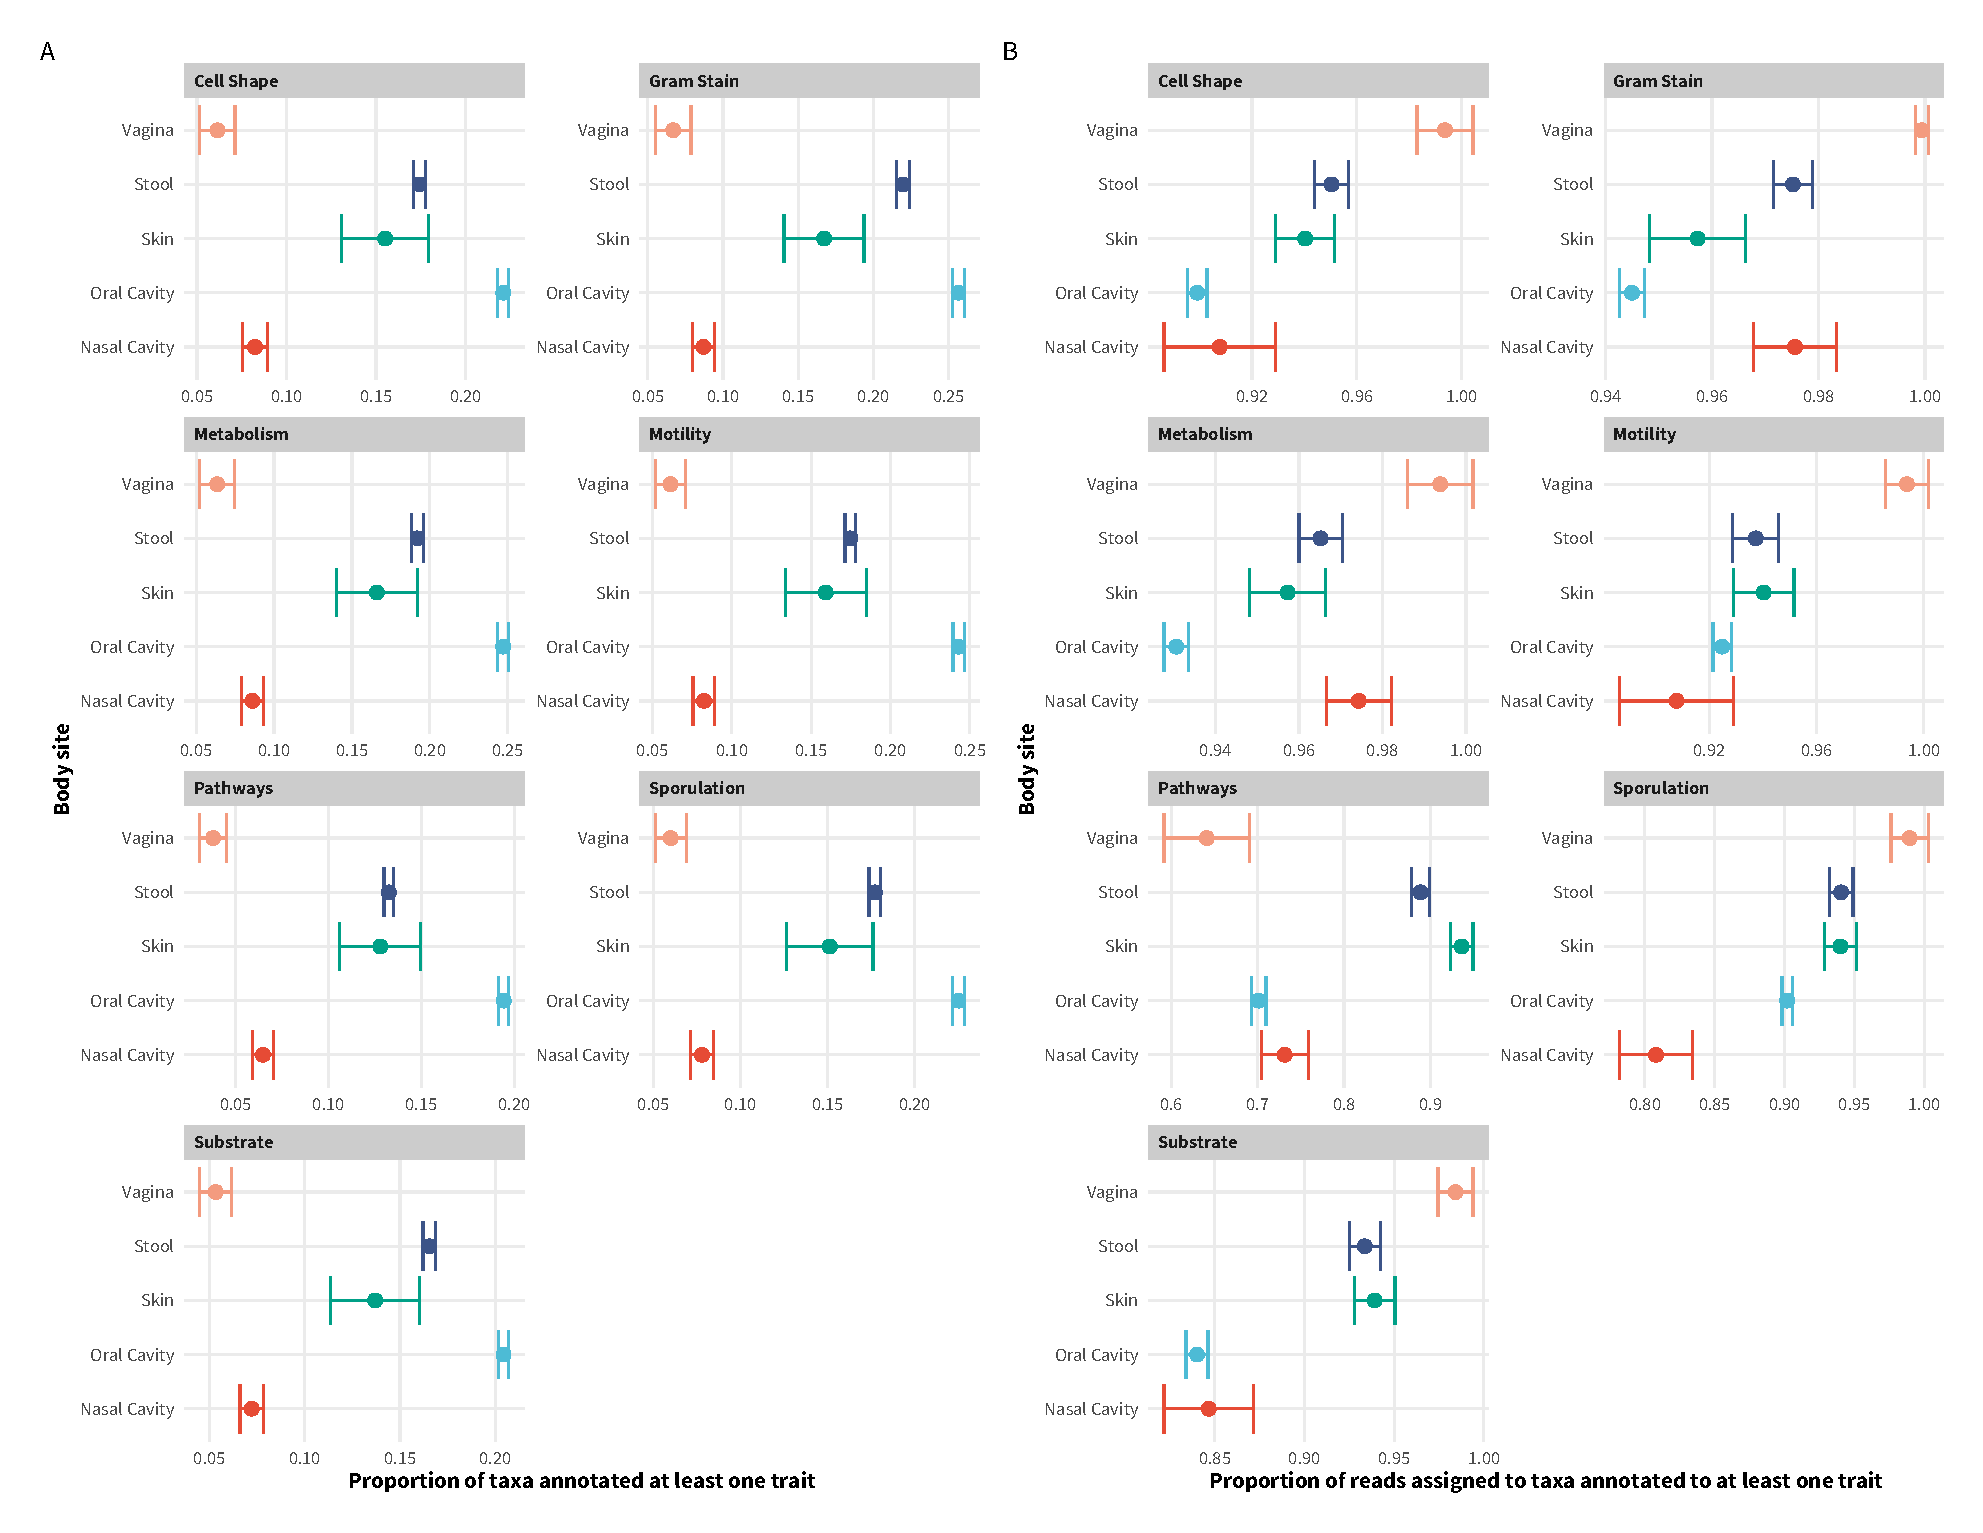
\includegraphics[width=0.99\linewidth]{figures/ch4_f1.eps}
\caption[Trait annotation coverage across different body sites for the HMP data set profiled using whole genome shotgun sequencing]{Trait annotation coverage across different body sites for the HMP data set profiled using whole genome shotgun sequencing. Panel \textbf{(A)} illustrates the proportion of present taxa per sample annotated to at least one trait. Panel \textbf{(B)} illustrates the proportion of reads assigned to taxa annotated to at least one trait which accounts for taxa relative abundances. Each plot facet represents different trait categories that were evaluated. Error bar represents the standard error of the evaluation statistic of interest across the total number of samples evaluated per body site.}
\label{fig:4.1}
\end{figure}

We also observed heterogeneity in the annotation coverage across different body sites and trait categories. For richness, nasal cavity and vaginal body sites were the lowest in coverage, with less than 5\% of taxa annotated with at least one trait across all trait categories while conversely, oral cavity sites consistently had the highest coverage under this metric. This pattern was reversed when considering coverage as the proportion of assigned reads per sample, but overall values were consistently high. Averaging coverage across body sites (Fig~\ref{fig:4.2}) also supports this observation, showing overall that the proportion of reads covered are similar across all body sites despite differences in the proportion of present taxa covered by trait annotations. Similar results were observed for sites profiled with 16S rRNA gene sequencing (Fig~\ref{fig:d1}), where oral sub-sites have the highest coverage across both richness and evenness metrics but, on average, all sites were similar in coverage statistics. Surprisingly, stool samples were low in coverage across multiple categories despite being one of the well studied systems. 

\begin{figure}[!h]
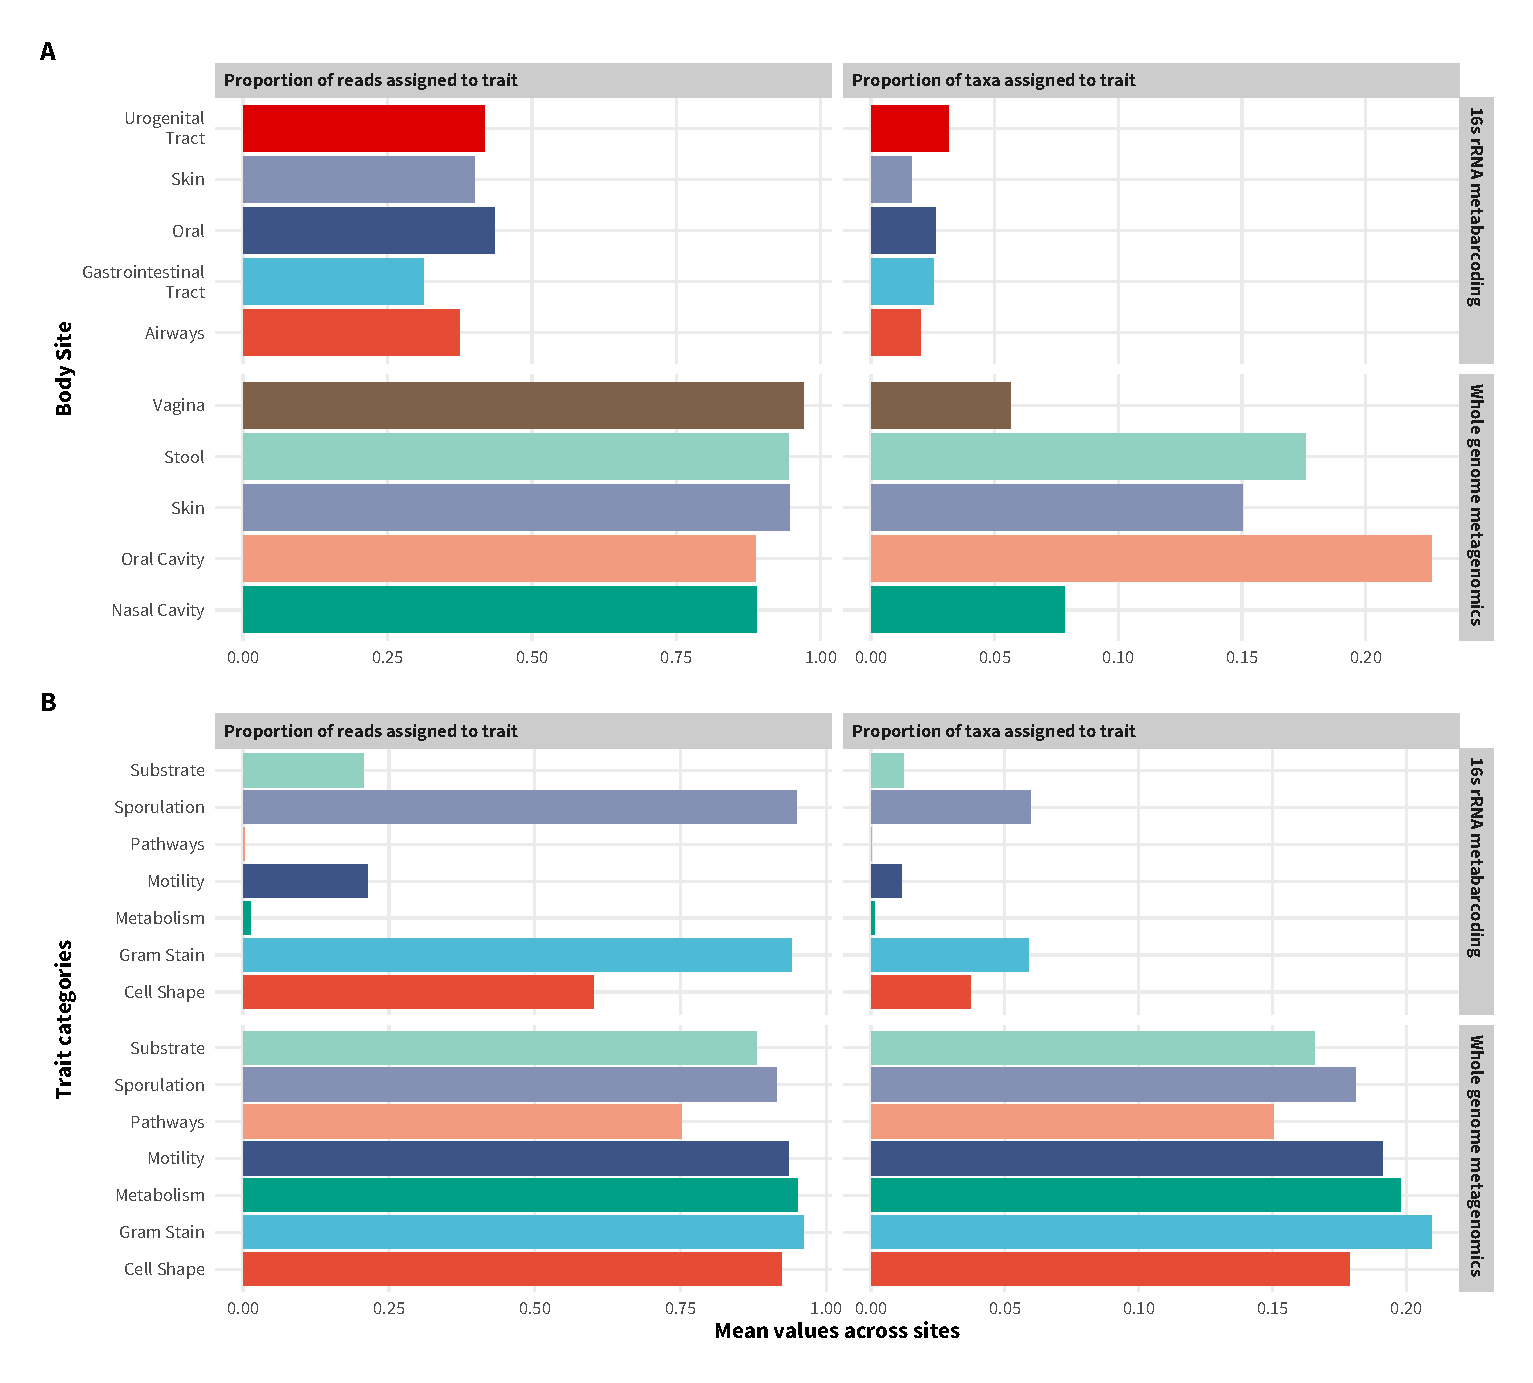
\includegraphics[width=0.99\linewidth]{figures/ch4_f2.eps}
\caption[Trait annotation coverage statistics for HMP data across samples profiled with both 16S rRNA gene metabarcoding and whole genome metagenomics]{Trait annotation coverage statistics for HMP data across samples profiled with both 16S rRNA gene metabarcoding and whole genome metagenomics. Panel \textbf{(A)} illustrates coverage statistics for each body site averaged across evaluated samples and trait categories. Panel \textbf{(B)} illustrates statistics for each trait category averaged across evaluated samples and body sites.}
\label{fig:4.2}
\end{figure}

We also stratified our coverage analyses by trait categories (Fig~\ref{fig:4.1}, Fig~\ref{fig:4.2}, Fig~\ref{fig:d1}). For samples profiled with whole genome sequencing, all trait categories are evenly covered, with about 15\% - 20\% of taxa were annotated to a trait of any category. However, these taxa comprise around 75\% to 100\% of the total reads per sample suggesting that the overall read level coverage is very high. However, in samples profiled with 16S rRNA gene sequencing, the overall coverage value across categories is low. Sporulation, substrate utilization and motility are the most covered category while pathways and metabolism has no coverage at all.  

\subsection{Predictive analysis} 
To determine the utility of trait-based sets, we generated enrichment scores for covered traits using CBEA \cite{nguyen2021cbea} for evaluated data sets and compared the predictive performance of using trait-set enrichment scores as inputs compared to alternative functional-based predictors. We evaluated two disease conditions, CRC and IBD, with data sets drawn from both 16S rRNA gene metabarcoding and whole genome metagenomic profiling techniques. We fitted a calibrated random forest model to each input type and computed predictive performance as AUROC (discriminatory power) and Brier scores (probability estimates) using 10-fold cross-validation.  

For the CRC prediction task, traits covered 2.7\% of taxa and 27.3\% of reads for the 16S rRNA gene metabarcoding data set, while for the whole genome sequencing data set, traits covered 9.1\% of taxa and 87.2\% of reads. For the IBD prediction task, traits covered 1.61\% of taxa and 26.7\% of reads for 16S rRNA gene metabarcoding data set, while for the whole genome sequencing data set, traits covered 6.6\% of taxa and 91.2\% of reads.  

Fig~\ref{fig:4.3} illustrates results of our model evaluations. Overall, enrichment scores for trait-sets are as good as other alternate function-based predictors at discriminating between case and control patients across both CRC and IBD conditions. Aside from pure discrimination power, models fitted on CBEA trait-set scores are also equivalent in approximating predicted probabilities. This is surprising especially for the 16S rRNA gene metabarcoding data sets, where the trait coverage is low. Even though the differences in performance is not significant, there are instances where trait-set scores perform slightly better than their pathway abundance counterparts. Since trait-features are also more descriptive, utilizing them can increase interpretation while also not scarificing performance.   

\begin{figure}[!h]
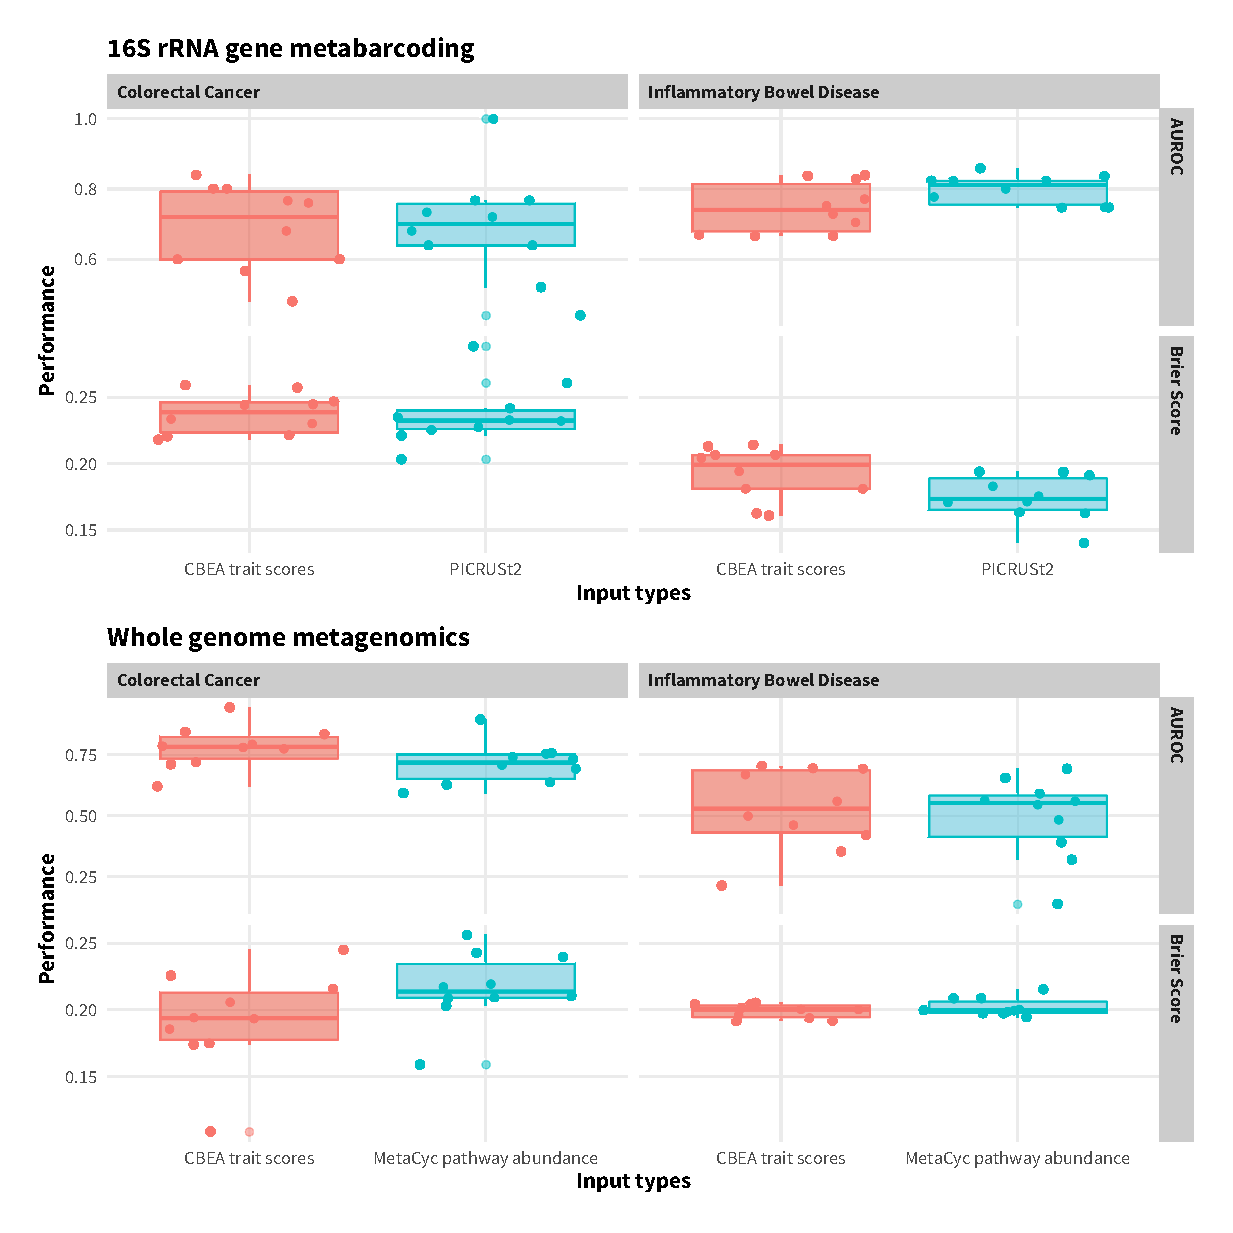
\includegraphics[width=0.99\linewidth]{figures/ch4_f3.eps}
\caption[Predictive performance of a calibrated random forest model across different disease conditions, profiling technique, and performance metrics]{Predictive performance of a calibrated random forest model across different disease conditions, profiling technique, and performance metrics. Scores were obtained via 10-fold nested cross validation where within each training fold there is a 10-fold cross validation procedure to calibrate predicted probabilities. For each condition and data type, CBEA trait-set scores were compared against MetaCyc pathway abundances from relevant sources (measured abundances for whole genome sequencing data sets and PICRUSt2 predicted abundances for 16S rRNA gene metabarcoding data sets)}
\label{fig:4.3}
\end{figure}

In addition to predicted performance, we also identified the top 10 features that are most important for model fitting. Since our model involves a 10-fold cross-validation procedure within the training set to calibrate predicted probabilities, top features are identified using the mean feature importance value across the 10 folds. Fig~\ref{fig:4.4} illustrates results for whole genome metagenomic data sets while Fig~\ref{fig:d2} illustrates results for the 16S rRNA gene metabarcoding data sets. Even though these are the top 10 features, the observed mean feature importance statistics are low, suggesting that no individual features were definitively the most important in discriminating between patient classes.  

\begin{figure}[!h]
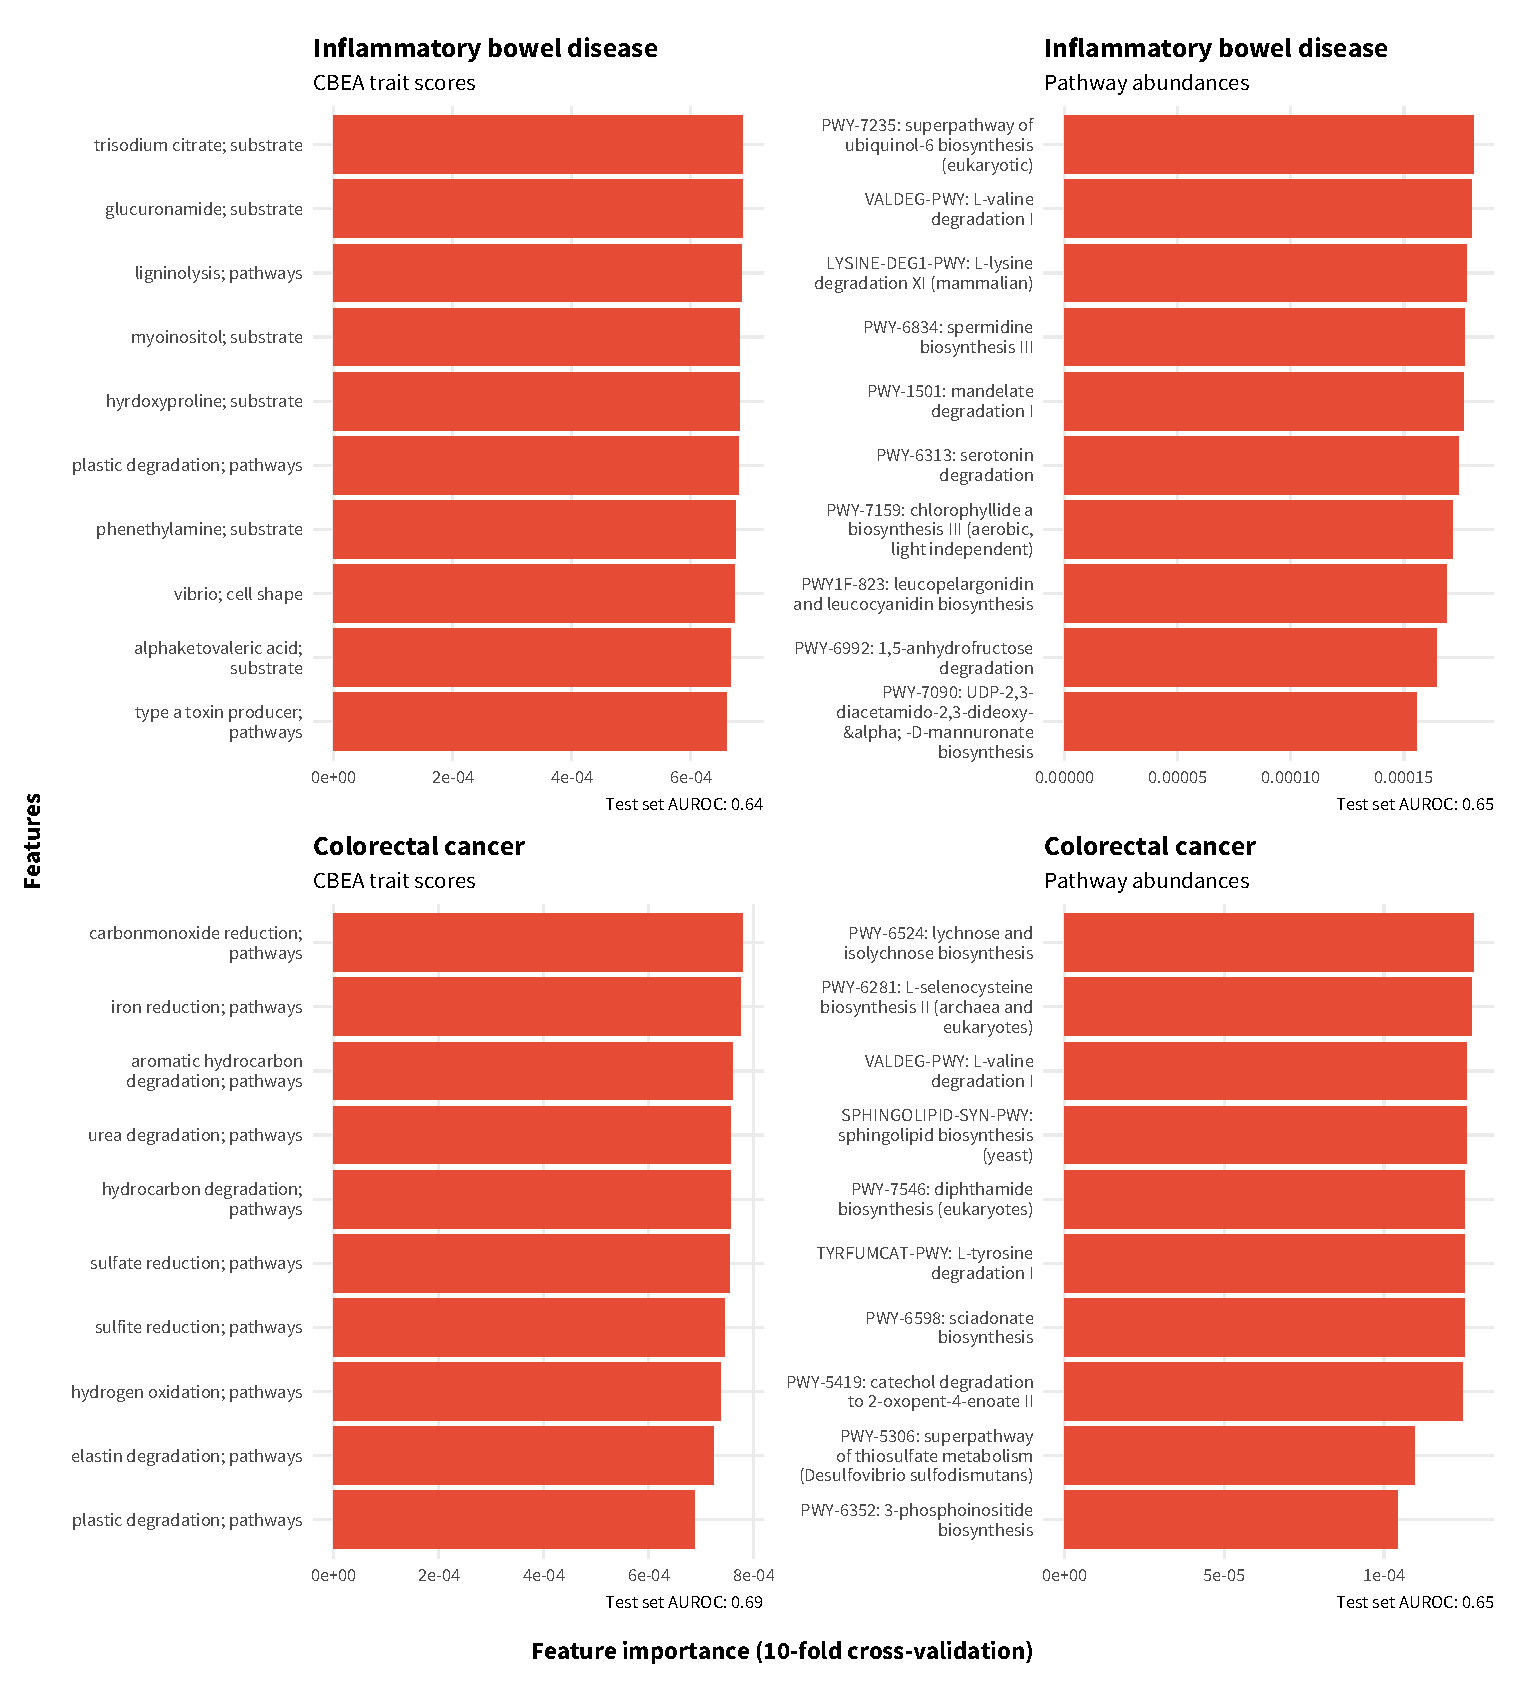
\includegraphics[width=0.99\linewidth]{figures/ch4_f4.eps}
\caption[Top 10 important features based on random forest model fitted different inputs from data sets profiled with whole genome metagenomics]{Top 10 important features based on random forest model fitted different inputs from data sets profiled with whole genome metagenomics. Features were selected from mean decrease in Gini impurity averaged across 500 decision trees and 10-fold cross-validation (nested with the training set) as implemented in \texttt{scikit-learn}. AUROC scored on a held-out test set is also presented for each input type and disease condition.}
\label{fig:4.4}
\end{figure}

\section{Discussion}
\subsection{Traits are annotated with high coverage at the species-level}

We computed the coverage of trait annotation on a typical dataset to understand the extent in which community function is captured, thereby serving as a proxy for expected confidence for an enrichment analysis performed using trait-based taxon sets. Low coverage in this case indicates that the database does not adequately capture the diversity of microbes found in the target data. This is because there might not be enough taxa present in the data set to serve as evidence for the trait. Alternately, this could also mean that the analysis is missing a majority of underlying community traits, many of which might be core to the health outcome association of interest but simply missing in the analysis. We computed coverage based on two metrics: first, a richness-like metric which computes coverage as the proportion of taxa present per sample annotated to a trait (for a given category and data set); second, an evenness-like metric that accounts for relative abundances of each annotated taxa by computing coverage as the proportion of reads per sample annotated to a trait.

When evaluated on the HMP data set (Fig~\ref{fig:4.1}), we can see that the overall richness coverage is low (less than 25\% of identified species) across all sites and data sets, particularly for nasal cavity and vaginal sub-sites. However, when considering evenness of coverage, almost all of reads were annotated to a trait. This is consistent with the observation that relative abundances of human-associated microbiomes are highly skewed \cite{consortium2012structure}, where a small number of species usually dominate the community. As such, even though traits might only cover a small number of taxa, they might represent the majority of community abundance. For example, Ravel et al. \cite{ravel2011vaginal} observed that \emph{Lactobacillus} species dominate the vaginal microbiome and, in some phylotypes, almost all reads are assigned to a single species. This shows that our trait-database has high degree of coverage across the most abundant taxon within a community, which supports utilizing these sets to perform exploratory analyses. However, low richness coverage also indicates that our database might not capture traits associated with rare taxa, which can play an important role in regulating host health \cite{velazquez2019endogenous}.

Unfortunately, coverage is significantly lower for samples profiled using 16S rRNA gene metabarcoding (Fig~\ref{fig:d1}). For some trait categories, such as pathways, no traits were assigned to any taxa (Fig~\ref{fig:4.2}). We hypothesized that this is due to two issues. First, metabarcoding data sets can only resolve taxonomies at the genus level \cite{johnson2019evaluation}, while traits are usually defined at the species and strain levels. Aggregating consensus traits to the genus is difficult due to the high degree of strain and species level diversity within the microbiome \cite{carrow2020strain}. Second, taxonomic assignments for metabarcoding data sets are often based amplification of a specific hyper-variable region for a marker gene (most often the 16S rRNA gene). This means that taxonomic assignment can be sensitive to the choice of region, and can be inaccurate. Furthermore, the choice of taxonomic database (e.g. Ribosomal Database Project \cite{cole2014ribosomal}, SILVA \cite{quast2013silva}) can also play a part in reducing the ability for trait annotation coverage. Differences between taxonomic paths \cite{balvociute2017silva} can result in certain taxa not being able to be matched to traits, which usually assign traits based on NCBI identifiers.  

\subsection{Trait-set features are predictive of disease outcomes}

We assessed the predictive performance of models fit on trait-set enrichment scores compared to other function-based inputs. For whole genome sequencing data sets, measured pathway abundances were utilized as a comparison point while for 16S rRNA gene sequencing data sets, predicted pathway abundances via PICRUSt2 were utilized instead. Fig~\ref{fig:4.2} shows that across all conditions and profiling techniques, trait-set features are competitive in producing well performing models and were able to discriminate between cases and controls. Surprisingly, performance was also comparable in the 16S rRNA gene sequencing data set despite overall low coverage across both richness and evenness metrics. This demonstrates that trait-set abundances can still provide an informative approximation to functional potential similar to PICRUSt2 that can be used for exploratory and hypothesis generating purposes.   

To determine which features are important for overall model performance, we extracted the top 10 features based on the mean decrease in Gini impurity. However, the overall feature importance values are not high, suggesting that no individual feature was dominant in classifying patient status. This is further supported by the fact that some nonsense features show up in the top 10 list for models fit using pathway abundances such as PWY-7235 and LYSINE-DEG-PWY, which are mammalian and eukaryotic pathways, respectively. However, the models still show respectable discriminatory power when evaluated on the test set (AUROC $\sim$ 0.7). Since random forest models can capture interactions between predictors \cite{hastie2009elements}, we hypothesized that the interaction between features contribute to test set performance rather than marginal effects. As such, we did not observe a high degree of feature importance scores since these measures are not designed to capture interaction effects \cite{wright2016little}. 

However, despite such limitations, we were still able to recover existing knowledge about the condition of interest. For example, ``sulfide reduction;pathways" was shown to be an important feature in discriminating subjects with CRC vs control subjects in Fig~\ref{fig:4.4}. This is supported by previous research showing that an increase in abundance of sulfate reducing bacteria is associated with the condition \cite{yachida2019metagenomic}. Mechanistically, this process, when using methionine or cysteine as substrates \cite{cheng2020intestinal}, generates H$_2$S as a product, which can stimulate CRC by inhibiting butyrate oxidation (which helps prevent the breakdown of the gut barrier) as well as promoting the generation of reactive oxygen species \cite{marquet2009lactate}. Another trait feature is ``urea degredation;pathways", which suggests the importance of bacterial-driven urea hydrolysis process, which is one of the main sources of ammonia in the human gut \cite{blachier2007effects}. Sustained exposure of colonocytes to free ammonia may contribute to the development of CRC \cite{clausen1992fecal}, which is supported by animal experiments showing histological damage in the distal colon after long-term ammonium exposure \cite{lin1991colon}.      
%\subsection*{Enrichment analyses using traits provide unique biological insights}
\subsection{Limitations and future directions}

Even though our results demonstrate that utilizing trait-based sets can provide meaningful insight to microbiome data sets, there are several major challenges to widespread adoption. Although trait databases do not suffer from the same types of biases that exist in genomic reference databases \cite{xu2014which}, the reliance on curated experimental data means that traits are usually only annotated for species that are well studied and culturable. While using predictive models can help in assigning traits to a broader category of taxa \cite{weimann2016genomes}, such automated approaches can result in misclassification of traits and increased noise in downstream analyses. Additionally, high-quality trait annotations require a time-consuming, manual curation process \cite{weissman2021exploring}. A source that is based on user submission such as GOLD \cite{mukherjee2021genomes} can cover a larger number of taxa and traits, but unfortunately can have erroneous and duplicated assignments due to the lack of a standardized nomenclature. There is currently a gap in producing a high-quality and diverse trait databases that are maintained and continuously updated.  

In addition to issues with trait database quality, there are also problems matching the identity of taxa in a given trait database with identifiers found in references for sequence-based taxonomic profiling such as SILVA \cite{quast2013silva}. For whole genome metagenomic data sets, standard tools (such as MetaPhlan \cite{beghini2021integrating}) can provide NCBI identifiers at the species or strain levels. However, it is currently unclear how to aggregate or disaggregate traits if the taxonomic resolution of the observed data set is higher or lower than that of the trait database in use. This is even more difficult with metabarcoding datasets, where low taxonomic resolution makes trait-to-taxa assignments sparse and less confident. 

Finally, there are also hurdles in being able to properly validate traits that are found to be significantly enriched due to a lack of ground truth data sets. While some traits can be matched to pathways directly, others involve complex coordination of multiple genetic pathways. As such, further investigation into ways to identify biological concordance between obtained results and external measurements can help improve confidence in utilizing traits for microbiome analyses. 


\section{Conclusion}

Set-based enrichment analysis is a useful approach for analyzing microbiome data sets since it not only reflects underlying biology but can also provide more unique perspectives of function that is linked to ecosystem services. Microbial trait databases are a promising resource to construct taxon-sets as traits represent physiological phenotypes. We demonstrated that trait-based sets have high coverage across body sites, especially for samples profiled using whole genome metagenomics. Furthermore, enrichment scores computed on such sets are also competitive in predicting case/control status compared to pathway abundances. As such, trait features found to be important in model fitting can be used to define interesting mechanistic hypotheses. 

% You can use the \nameref{label} command to cite supporting items in the text.

%\clearpage

\section{Availability of data and materials}
All data sets are available publically via \texttt{Qiita}, \texttt{HMP16SData}, and \texttt{curatedMetagenomicData} with raw sequence data available on NCBI in their respective project repositories. All analysis scripts and generated figures are available on GitHub (\url{https://www.github.com/qpmnguyen/microbe_set_trait}). 

\section{Acknowledgements}
The authors thank Becky Lebeaux for insightful comments that greatly improved the paper. We would also like to thank maintainers of the packages \texttt{curatedMetagenomicData}, \texttt{HMP16SData}, \texttt{phyloseq}, \texttt{QIIME2}, \texttt{Qiita}, \texttt{TreeSummarizedExperiment} for all their efforts in maintaining open source repositories for data analysis and data sharing.  




\chapter{Conclusion}

Taxa-function relationships are difficult to characterize due to the different scales in which they operate \cite{langille2018exploring}. For the taxonomic layer, one can look at species, strain, or even cell states \cite{mcnulty2021dropletbased}. For the functional layer, it can be gene family abundance, transcript expression, or metabolite concentrations. Each degree of granularity increases the complexity of both the data collection process as well as its interpretation. Unfortunately, due to the byzantine nature of the microbiome, no approach is uniquely ``wrong", and can in fact reveal unique perspectives. As such, this thesis attempts to move the dial slightly by considering various distinct ways to decipher taxa-function relationships and evaluate their utility. 

\section{Summary of findings}
\subsection{Mapping microbes to their function using multi-omics data}

In chapter 2, we examined a paired metataxonomic-metabolomic data set to explore the relationship between bacterial relative abundances and metabolite concentrations. Even though multi-omics studies involving metabolomics are not new \cite{lloyd-price2019multiomics, ayeni2018infant, kisuse2018urban}, most studies have focused on defining differences between subject case/control status, with limited exploration of the microbe-metabolite interface. Here, we characterized associations between the microbiome (profiled using 16S rRNA gene sequencing) and the metabolome (profiled using NMR techniques). The analyzed metabolomic data set contained both untargeted taxonomic bins, as well as  concentrations of 36 specific metabolites. This data was generated for a cohort of healthy infants from the NHBCS with samples collected at 6-weeks and 12-months of age. 

Using both procrustes and sCCA, we found that overall metabolite concentrations are concordant with genus-level taxonomic profiles. This relationship is weakly predictive, as we observed poor performance across different machine learning models using predictive R-squared as the evaluation metric. However, model outputs performed better using Spearman correlation $\rho$, but still lower compared to other studies using a similar performance metric \cite{mallick2019predictive}. Using $\rho = 0.3$ as a threshold for defining ``well-predicted" metabolites \cite{mallick2019predictive, muller2021metaanalysis}, we found that SFCAs such as butyrate are most predictive, consistent with our understanding of microbiome physiology \cite{leblanc2017beneficial}. Surprisingly, the degree of coupling is higher for infants at 6-weeks compared to 12-months, suggesting that in early life humans are more reliant on the microbiome for metabolic purposes. 

In addition to overall patterns of associations, we also identified genera-metabolite groups that are core to the overall multivariate correlation by looking at the non-zero loading coefficients of our sCCA model. Similar to our concordance analysis, two SCFAs Butyrate and Proprionate were selected as the most important for the overall microbiome-metabolome relationship, with a surprising negative correlation with \emph{Bifidobacterium} genera, a commonly identified producer of SCFAs \cite{james2019metabolism}. We hypothesized that this is an instance of strain-level variation where some strains of \emph{Bifidobacterium} compete with other butyrate-producing taxa \cite{riviere2016bifidobacteria}. Amino acids were also well-represented among selected metabolites and were negatively correlated with taxa abundances. We hypothesized that microbes are incorporating amino acids in their environment directly instead of catabolizing them due to the fact that this process is energetically inefficient \cite{franzosa2014relating, oliphant2019macronutrient}. 

Our study showed that genus level microbial abundances are not sufficient to predict metabolite concentrations. However there is still a degree of overall coupling that is supported by prior work \cite{ayeni2018infant, kisuse2018urban, zierer2018fecal}. Additional studies with higher taxonomic resolution using whole genome metagenomics can be used to find more granular scales of association. We also provide further evidence to support the importance of microbiome-mediated butyrate catabolism in early life, while also suggesting that amino acids might play an important role. However, our study is limited by our cross-sectional design. This is because metabolite abundances are always changing, making measures of flux (or rate of change) more meaningful in finding associations \cite{hollywood2006metabolomics}. Some studies have attempted to bridge this gap using genome-scale metabolic models \cite{noecker2019defining}, which can be fit to observed data. However, additional studies with dense longitudinal sampling are still needed.   

\subsection{Developing novel methods to integrate taxa-function relationships in statistical analyses}

In chapter 3, we developed a statistical method to test for the enrichment of groups of microbes. Gene set testing (or pathway analysis), is a commonly utilized in the genomics literature to aggregate lists of genes obtained after a differential abundance test \cite{irizarry2009gene, goeman2007analyzing}. These methods have been shown to improve power, reproduciblity, and interpretability \cite{khatri2012ten}. As such, set-based analysis can be a useful method to not only address some of the challenges of analyzing sequencing-based taxonomic data tables (such as sparsity) \cite{li2015microbiome}, but also to provide a formal statistical approach to incorporate taxa and function via sets. Here, we provide a method for set-based enrichment analysis called CBEA that is tailored to microbiome relative abundance data. CBEA generates sample-level scores in an unsupervised manner by integrating the $Q_1$ competitive null hypothesis \cite{tian2005discovering} and compositional balances \cite{silverman2017phylogenetic, egozcue2003isometric}. Inference is performed at the sample-level through estimating an empirical null distribution that can be adjusted for variance inflation. 

We evaluated our model using both real and simulated data sets. First, CBEA can be used to test for enrichment at the sample level. Results indicated that our approach was able to control for type I error at the appropriate $\alpha$ level, however, the trade off is limited power to detect small effect sizes, especially at higher degrees of inter-taxa correlation. In addition, CBEA can also perform population-level analyses to detect sets that are differentially abundant between case/control status by combining generated scores with a difference in means test (such as Welch's t-test). Under this task, CBEA was able to control well for type I error but without having to concede as much power. Notably, CBEA produces fewer false positives compared to using a sum-based approach to aggregate taxa to sets and performing a standard differential abundance test such as \texttt{corncob} \cite{martin2020modeling}. Finally, even though CBEA generated scores were informative for discriminating between healthy controls and patients with IBD, performance scores were not significantly higher than other comparison methods.  

Our study illustrates an example of a statistical method that can assist in generating taxa-function hypotheses through the use of set annotations. Using CBEA, users can not only perform inference, but also use CBEA sample scores for downstream analyses such as predictive modeling, sample ordination, or network analysis. However, additional follow-up approaches are required to improve the inference procedure, as well address data sparsity beyond pseudocounts. 

\subsection{Leveraging existing microbiology knowledge to define microbial ecosystem roles}

In chapter 4, we explored using an aggregated database of microbial traits defined based on laboratory experiments to curate function-based taxon sets. 

\section{Perspectives and future research}

This thesis has explored different avenues to tackle identifying relevant taxa-function relationships and leverage them in standard epidemiological studies. As a result, we can provide more contextualized interpretations of microbes in differential abundance analyses and subsequently derive mechanistically meaningful hypotheses. This can help focus the efforts of follow-up laboratory validation studies. However, there are still major hurdles before an integrative taxa-function framework can be confidently applied to future studies. 

\subsection{Defining microbial function}

One of the most difficult aspects of investigating microbial function is the ability to define relevant microbial functions \cite{heintz-buschart2018human, zhang2019advancing, klassen2018defining}. Specifically, the question of how to translate between definitions of genes and pathways (from KEGG or MetaCyc) to ecosystem functions that the gut microbiome delivers. A relevant example is the role of HMO metabolism \cite{vatanen2018human}, which is a host-relevant function that is easily connected to their molecular origins. 

Chapter 4 of this thesis attempted to examine function under the lens of microbial traits. Traits are usually conceptualized as defined, measurable properties of organisms that link performance and contribution to core ecosystem needs \cite{krause2014traitbased}. While traits provide a more holistic conception of function, issues with unstandardized databases \cite{madin2020synthesis} and limited coverage for rare species makes it difficult to translate its usage to all studies. 

As such, comprehensive efforts are needed to centralize and standardize the ontology of microbial function with respect to ecosystem needs. Efforts such as the ontology of microbial phenotypes (OMP) \cite{chibucos2014ontology} have started to generate a repository of terminology to standardize description of microbial phenotypes. Researchers can further expand the types of annotations of OMP to be specific to body sites (using the uber-anatomy ontology - UBERON) or study conditions (using experimental factor ontology - EFO). KEGG terms or MetaCyc pathways can be assigned to OMP annotations, which can then be translated to specific strains using reference genomes/pangenomes or measured metatranscriptomic data. By defining a standardized vocabulary, we can begin to conceptualize a host-centric view of microbial function that is both standardized and context driven. 

\subsection{Leveraging multiple meta`omic technologies}

While there have been a large number of microbiome multi-omic studies (see section 1.2.2), they have mostly been focused on analyzing each data-layer independently with some studies performing limited taxa-function analyses. However, as shown in Chapter 2, paired profiling of microbiome structure and molecular functions can reveal novel aspects of host-microbe interactions. As such, multi'omic data sets, especially those including multiple layers of functional profiling, can be invaluable. 

Additionally, these data sets can be further leveraged in conjunction with the functional framework defined above in two ways: 

\begin{itemize}
    \item First, researchers can use these data sets directly to test for the enrichment of ecosystem-specific functional roles similar to that of Vatanen et al. \cite{vatanen2018human} and HMO metabolism. 
    \item Second, researchers can leverage the collection of these data sets to validate encoded taxa-function relationships, specifically accounting for situations where gene carriage does not directly correlate with expression \cite{franzosa2014relating}
\end{itemize}

\subsection{Novel representations of taxa-function relationships}

To jointly test for association between taxa-function groups and relevant exposures or disease outcomes, there is a need to identify appropriate representations that can be translated into a statistical framework. Set-based approaches, used in Chapter 3, are simple but powerful methods. Sets naturally capture categorical information such as the assignment of strains to functions. However, the definition of sets are rigid, and does not account for nuances such as uncertainties or the degree of strain presence/absence in the overall population. As such, novel numerical representations of taxa-function relationships can help account for this gap and allow for a more flexible way to encode these relationships. 

One candidate would be to use weights within sets or across different sets depending on the experimental context. For example, Frost \cite{frost2018computation} curates a set of tissue-specific weights MSigDB gene sets. Here, we can compute body-site specific weights for each functional term, or to weight the contribution of each taxa by its prevalence estimated from a large cohort such as HMP.  

Network-based methods offer another approach. Bipartite networks can be used to model connections between taxonomic and functional nodes \cite{tian2020decipheringa}. Networks also have topological features such as degree centrality that can provide extra dimensions such as being able to identify taxa that contribute to a large number of functions or vice versa. Utilizing standard networks that allow for connections within taxonomic and functional nodes can also allow researchers to account for inter-taxa correlation or dependencies between metabolites or genes. 

There are also machine-learning based approaches that can provide unique encoding opportunities. Word embeddings, such as Word2Vec \cite{mikolov2013efficient}, create dense numerical vectors that can represent high-dimensional co-occurrence relationships. This application has been explored in the context of the microbiome-metabolome relationship \cite{morton2019learning}. Researchers can extend this approach to model different functional outputs, or to provide pre-trained embeddings based on a meta-analysis of microbiome-metabolome data sets.  

%\chapter{Sample Decent Chapter Title}

Every good story begins with a twist. Let's test it out and see how it goes. Beginning to ending, just spin around! Every good story begins with a twist. Let's test it out and see how it goes. Beginning to ending, just spin around! Every good story begins with a twist. Let's test it out and see how it goes. Beginning to ending, just spin around! Every good story begins with a twist. Let's test it out and see how it goes. Beginning to ending, just spin around! Every good story begins with a twist. Let's test it out and see how it goes. Beginning to ending, just spin around! Every good story begins with a twist. Let's test it out and see how it goes. Beginning to ending, just spin around! Every good story begins with a twist. Let's test it out and see how it goes. Beginning to ending, just spin around! Every good story begins with a twist. Let's test it out and see how it goes. Beginning to ending, just spin around!

\section[Shorter Title]{Section with an Unnecessarily Long Title}

Every good story begins with a twist. Let's test it out and see how it goes. Beginning to ending, just spin around! Every good story begins with a twist. Let's test it out and see how it goes. Beginning to ending, just spin around! Every good story begins with a twist. Let's test it out and see how it goes. Beginning to ending, just spin around! Every good story begins with a twist. Let's test it out and see how it goes. Beginning to ending, just spin around! Every good story begins with a twist. Let's test it out and see how it goes. Beginning to ending, just spin around! Every good story begins with a twist. Let's test it out and see how it goes. Beginning to ending, just spin around! Every good story begins with a twist. Let's test it out and see how it goes. Beginning to ending, just spin around! Every good story begins with a twist. Let's test it out and see how it goes. Beginning to ending, just spin around!

\subsection{Example of a subsection}

Every good story begins with a twist. Let's test it out and see how it goes. Beginning to ending, just spin around! Every good story begins with a twist. Let's test it out and see how it goes. Beginning to ending, just spin around! Every good story begins with a twist. Let's test it out and see how it goes. Beginning to ending, just spin around! Every good story begins with a twist. Let's test it out and see how it goes. Beginning to ending, just spin around! Every good story begins with a twist. Let's test it out and see how it goes. Beginning to ending, just spin around! Every good story begins with a twist. Let's test it out and see how it goes. Beginning to ending, just spin around! Every good story begins with a twist. Let's test it out and see how it goes. Beginning to ending, just spin around! Every good story begins with a twist. Let's test it out and see how it goes. Beginning to ending, just spin around!

\subsubsection{Subsubsections, the final formatted heading}

Every good story begins with a twist. Let's test it out and see how it goes. Beginning to ending, just spin around! Every good story begins with a twist. Let's test it out and see how it goes. Beginning to ending, just spin around! Every good story begins with a twist. Let's test it out and see how it goes. Beginning to ending, just spin around! Every good story begins with a twist. Let's test it out and see how it goes. Beginning to ending, just spin around! Every good story begins with a twist. Let's test it out and see how it goes. Beginning to ending, just spin around! Every good story begins with a twist. Let's test it out and see how it goes. Beginning to ending, just spin around! Every good story begins with a twist. Let's test it out and see how it goes. Beginning to ending, just spin around! Every good story begins with a twist. Let's test it out and see how it goes. Beginning to ending, just spin around!

\section{A Second Section}

Every good story begins with a twist. Let's test it out and see how it goes. Beginning to ending, just spin around! Every good story begins with a twist. Let's test it out and see how it goes. Beginning to ending, just spin around! Every good story begins with a twist. Let's test it out and see how it goes. Beginning to ending, just spin around! Every good story begins with a twist. Let's test it out and see how it goes. Beginning to ending, just spin around! Every good story begins with a twist. Let's test it out and see how it goes. Beginning to ending, just spin around! Every good story begins with a twist. Let's test it out and see how it goes. Beginning to ending, just spin around! Every good story begins with a twist. Let's test it out and see how it goes. Beginning to ending, just spin around! Every good story begins with a twist. Let's test it out and see how it goes. Beginning to ending, just spin around!
\appendix
\chapter{List of abbreviations}

NHBCS: New Hampshire Birth Cohort Study
NMR: Nuclear Magnetic Resonance
PCoA: Principal Coordinates Analysis
gUniFrac: Generalized Unique Fraction 
ASV: Amplicon Sequence Variant
FDR: False Discovery Rate
sCCA/CCA: Sparse Canonical Correlation Analysis
SCFA: Short Chain Fatty Acids
RF: Random Forest
EN: Elastic Net
SVM-RBF: Support Vector Machines with Radial Basis kernel Function
SPLS: Sparse Partial Least Squares
CLR:  Centered Log Ratio transformation
\chapter{Supporting material for ``Associations between the gut microbiome and metabolime in early life"}

\section{List of abbreviations}

\section{Supplemental Notes} 
\paragraph{Supplementary Note 1}
\label{appB_note1}
{\bf Microbe-metabolite participation in significant pairwise Spearman correlation}. Univariate pairwise Spearman correlations were performed to identify significant microbe-metabolite pairs. Significance was determined by the Spearman false discovery rate (FDR) threshold of 0.05 following a Benjamini-Hochberg multiple hypothesis testing procedure.  At both time points a majority of genera and metabolites were significantly correlated, where at 6 weeks, 28 genera (65\% of total genera) and 36 metabolites (100\% of metabolites) were part of 516 significant correlations (16.6\% of total pairwise comparisons) while at 12 months, 59 genera (81.9\% of total genera) and 29 metabolites (80\% of metabolites) were involved in 214 significant correlations (8.01\% of total pairwise comparisons). This result also supported the observation that at 6 weeks the microbiome was marginally more associated with the metabolome compared to 12 months. Similar to sCCA results, untargeted data set showed a similar signal at both time points. Specifically, at 6 weeks, 37 genera (86\% of genera) and 198 metabolite bins (95.1\% of bins) were part of 1480 significant associations (16.5\% of pairwise comparisons). Similarly, at 12 months, 67 genera (93\% of genera) and 207 metabolite bins (99.5\% of bins) were part of 1392 significant associations (9.2\% of total pairwise comparisons). 

\paragraph{Supplementary Note 2}
\label{appB_note2}
{\bf Sparse canonical correlation analysis selects microbes and metabolites important to the inter-omic correlation.} Only a small subset of metabolites and microbes were selected (27\% of taxa for both time points; 16.9\% of metabolites at 6 weeks and 19.4\% of metabolites at 12 months). At both time points, selected taxa belong to the Firmicutes, Actinobacteria and Proteobacteria phyla with Firmicutes being the most represented (58.3\% of selected taxa at 6 weeks; 70\% of selected taxa at 12 months). Actinobacteria was the second most selected phylum (25\% of selected taxa) at 6 weeks while at 12 months it was Proteobacteria (30\% of selected taxa). For metabolites, amino acids were the most represented metabolite class (Table~\ref{tab:b1}) (60\% of selected metabolites at 6 weeks, 85\% of selected metabolites at 12 months). 6-week samples demonstrated a larger diversity of metabolite classes, with additional representatives from carboxylic acids group, nucleotides and short chain fatty acids (SCFA) while at 12 months, the only non-amino-acid metabolite is uracil (of the nucleotide class). Across both time points, 3 genera (Flavonifractor, Haemophilus and Acinetobacter genera) and 5 metabolites (lysine, isoleucine, leucine, uracil, phenylalanine) were consistently selected. Surprisingly, in the untargeted analysis, nearly half of taxa and metabolites were selected at 6 weeks while the number remained more similar to the targeted analysis at 12 months (6 weeks: 46\% of taxa and 42\% of metabolite bins; 12 months: 13.8\% of taxa and  17.3\% of metabolite bins). However, the taxonomic distribution of those selected taxa remained similar, with Firmicutes being the most dominating phyla (60\% of selected taxa at both time points). Additionally, for both time points, the sign of the sCCA loadings for selected variables were also concordant with patterns of negative and positive correlation via univariate Spearman correlations (Figure 3, right panels). Notably, all selected metabolites contain negative loadings for both time points, with the majority of selected pairwise correlation to be negative (6 weeks: 76.6\% of selected pairwise comparisons, 12 months: 60.7\% of selected pairwise comparisons). This pattern is replicated in the untargeted data set as well (6 weeks: 61.3\% of selected pairwise comparisons, 12 months: 70\% of selected pairwise comparisons). 

\paragraph{Supplementary Note 3}
\label{appB_note3}
\textbf{Prediction results.} Under $R^2$, at 6 weeks only 8 (22.2\%) metabolites (Butyrate, Glycerol, Isobutyrate, Isoleucine, Leucine, Methionine, Phenylalanine and Tyrosine) were predictable, with a mean of 4.85\% and a maximum of 11.8\% (Butyrate using EN). At 12 months, only 14 (38.9\%) of metabolites (Butyrate, Formate, Inosine, Isobutyerate, Isoleucine, Lactate, Leucine, Methionine, Phenylalanine, Propionate, Propylene glycol, Tyrosine, Uracil, Valine) were predictable, with a mean of 4.81\% and a maximum of 8.7\% (Propylene Glycol using RF). When looking at the average R2 across all metabolites, performance was not good (-5.6\% at 6 weeks; -3.07\% at 12 months). This negative $R_2$ value implies that the predicted model performs worse than the naïve, intercept only model. Conversely, correlative performance was much better. At 6 weeks 26 metabolites (83\%) were predictable, with a mean correlation of 0.344 and a maximum of 0.669 (Butyrate using EN). Similarly, at 12 months all 36 targeted metabolites were predictable, with a mean of 0.265 and a maximum of 0.549 (Succinate using EN). Using the SCC cutoff of 0.3 as criteria for well predicted metabolites, many metabolites at 6 weeks were still retained (25 metabolites - 69.4\%). Conversely, at 12 months, only 13 metabolites remained to be well predicted (38.9\%). On average, performance based on SCC was good with a mean SCC value of 0.339 at 6 weeks and 0.249 at 12 months. In the untargeted analysis looking at the entire metabolome, performance was much better for both metrics. Under R2, 116 (56.7\%) of metabolite bins were predictable at a maximum of 42.7\% (Bin 33 using SPLS) and a mean of 16.7\% at 6 weeks while at 12 months, 94 (45.1\%) of metabolite bins were ell predicted at a maximum of 22.7\% (Bin 16 using SVM) and a mean of 8.19\%. The overall average across all metabolites is 3.91\% (6 weeks) and -0.59\% (12 months). This trend was similarly observed using SCC, as all all 208 metabolites bins were predictable for both time points (using SCC = 0 as the threshold). Specifically, of the predictable metabolites at 6 weeks the maximum value was 0.687 (Bin 32 using EN) with a mean of 0.352 while at 12 months, the maximum value was 0.53 (Bin 16 using SVM) and a mean of 0.253. Using the SCC cutoff of 0.3 as above, at 6 weeks 120 metabolite bins (57\% of bins) were well predicted while at 12 months only 60 (28.8\% of bins) were well predicted.


\section{Availability of data and materials}

The 16S rRNA gene sequencing datasets used in this study are stored in the National Center for Biotechnology Information (NCBI) Sequence Read Archive: \url{http://www.ncbi.nlm.nih.gov/sra} under accession number PRJNA296814. The raw and processed metabolomics data is available at the NIH Common Fund's National Metabolomics Data Repository (NMDR) website, the Metabolomics Workbench, \url{https://www.metabolomicsworkbench.org} where it has been assigned Project ID PR001146. The data can be accessed directly via its project DOI: \url{https://doi.org/10.21228/M8K69N}. All intermediary analysis objects and scripts are available on GitHub. 

\section{Supplemental tables}

Table S1. Metabolites selected for targeted analysis and their potential biological functions.

Table S2: Primers used for bacterial 16S rRNA gene sequencing 

\section{Supplemental figures}

\begin{figure}
    \centering
    %\includegraphics{}
    \caption[Inter-omics Procrustes biplots comparing PCoA ordinations of untargeted metabolite profiles and taxonomic relative abundances for 6 weeks (left panels) (n = 158) and 12 months (right panels) (n = 262).]{Inter-omics Procrustes biplots comparing PCoA ordinations of untargeted metabolite profiles and taxonomic relative abundances for 6 weeks (left panels) (n = 158) and 12 months (right panels) (n = 262). Top panels present analyses based on ordinations from Euclidean distances of genus level abundances after centered log ratio transformation and Euclidean distances of arcsine square root transformed metabolite relative abundances. Bottom panel presents analyses based on generalized Unifrac distance of amplicon sequence variant (ASV) relative abundances and Euclidean distances of arcsine square root transformed metabolite relative abundances.}
    \label{fig:b1}
\end{figure}

\begin{figure}
    \centering
    %\includegraphics{}
    \caption[Pairwise Spearman correlation of metabolite bins and genus-level taxonomic abundances for 6-weeks (panel A, N = 158) and 12-months (panel B, N = 282) infants.]{Pairwise Spearman correlation of metabolite bins and genus-level taxonomic abundances for 6-weeks (panel A, N = 158) and 12-months (panel B, N = 282) infants. Left panel displays the overall correlation pattern, where non-significant correlations are not colored (false discovery rate (FDR) controlled q-value < 0.05). Right panel displays the same heatmap restricted to taxa and metabolites selected by the sparse CCA procedure. Additionally, correlation coefficient of the first sCCA variate pair, bootstrapped 95\% confidence interval and permutation p-value are also reported.}
    \label{fig:b2}
\end{figure}

\begin{figure}
    \centering
    %\includegraphics{}
    \caption[Comparative analysis predictive model performance across all metabolites in the untargeted dataset for both 6-weeks (n = 158) and 12-months (n = 282) timepoints.]{Comparative analysis predictive model performance across all metabolites in the untargeted dataset for both 6-weeks (n = 158) and 12-months (n = 282) timepoints. Top panel shows superimposed boxplots and violin plots of the distribution of predictive posterior mean for each evaluation metric across all 208 spectral bins. Bottom panels show aggregated model rankings for all metabolites using R-squared (left) and spearman correlation (right) using Borda scores (Methods).}
    \label{fig:b3}
\end{figure}


Figure S4. Results for positive (Panel A) and negative simulations (Panel B). Positive simulations were conducted based on bootstrapped resamples of the original data (12-month time point) and a normally distributed outcome vector which represented a log-transformed metabolite profile. Different levels of model saturation (horizontal, model sparsity (spar) at 0.05, 0.1, 0.5, 0.95) and effect sizes (vertical, signal-to-noise ratio (snr) at 0.5, 0.7, 3, 5) were assessed, with 100 data sets generated for each setting combination. Negative simulations were conducted based on permutations of the original data (12-month time point), with a total of 1000 permutations. Highly negative outliers were removed for the purposes of visualization
Figure S5. Inter-omics Procrustes biplots comparing PCoA ordinations of targeted metabolite profiles and taxonomic relative abundances in the sensitivity analyses for 6 weeks (left panels) (n = 65) and 12 months (right panels) (n = 65). Top panels present analyses based on ordinations from Euclidean distances of genus level abundances after centered log ratio transformation and Euclidean distances of arcsine square root transformed metabolite relative abundances. Bottom panel presents analyses based on generalized Unifrac distance of amplicon sequence variant (ASV) relative abundances and Euclidean distances of arcsine square root transformed metabolite relative abundances
Figure S6. Inter-omics Procrustes biplots comparing PCoA ordinations of untargeted metabolite bin relative concentrations and taxonomic relative abundances in the sensitivity analyses for 6 weeks (left panels) (n = 65) and 12 months (right panels) (n = 65). Top panels present analyses based on ordinations from Euclidean distances of genus level abundances after centered log ratio transformation and Euclidean distances of arcsine square root transformed metabolite relative abundances. Bottom panel presents analyses based on generalized Unifrac distance of amplicon sequence variant (ASV) relative abundances and Euclidean distances of arcsine square root transformed metabolite relative abundances
Figure S7. Pairwise spearman correlation of concentration-fitted targeted metabolite concentrations and genus-level taxonomic abundances for 6-weeks (panel A, N = 65) and 12-months (panel B, N = 65) infants in sensitivity analyses. Left panel displays the overall correlation pattern, where non-significant correlations are not colored (FDR controlled q-value < 0.05). Right panel displays the same heatmap restricted to taxa and metabolites selected by the sCCA procedure. Additionally, correlation coefficient of the first sCCA variate pair, bootstrapped 95\% confidence interval (nboot = 5000) and permutation p-value (nperm = 1000) are also reported.
Figure S8. Pairwise spearman correlation of untargeted metabolite bin relative concentrations and genus-level taxonomic abundances for 6-weeks (panel A, N = 65) and 12-months (panel B, N = 65) infants in sensitivity analyses. Left panel displays the overall correlation pattern, where non-significant correlations are not colored (FDR controlled q-value < 0.05). Right panel displays the same heatmap restricted to taxa and metabolites selected by the sCCA procedure. Additionally, correlation coefficient of the first sCCA variate pair, bootstrapped 95\% confidence interval (nboot = 5000) and permutation p-value (nperm = 1000) are also reported
Figure S9: Spearman correlation coefficients and 95\% confidence intervals of significant correlations (q-value < 0.05) between metabolite concentrations in the targeted data set and the abundances of pathways that produce them. Pathway abundances were obtained via PICRUSt2 predictions, with pathway-metabolite relationship retrieved from MetaCyc database. Both 6-week (n = 158) and 12-month (n = 282) samples are represented
Figure S10. Top five contributors at the Genus level for each significantly correlated pathway-metabolite pair obtained using observed metabolite concentrations and predicted pathway abundances (spearman correlation with q-value < 0.05). Panel A represents 6-week samples while panel B represents samples at 12-months. Relative contributions are calculated as the total number of copies of genes mapped to a pathway across all samples per Genus over the total number of gene copies assigned to that pathway. 
Figure S11. Heatmap representing overall spearman correlations between predicted pathway abundances (obtained via PICRUSt2) and metabolite concentrations in the targeted data set regardless of pathway-metabolite annotations. Both 6-week (n = 158) (Panel A) and 12-month (n = 282) (Panel B) samples are presented. Non-significant correlations (q-value > 0.05) are not colored. 

\chapter{Appendix C: Supporting material for ``Evaluating trait databases for taxon set enrichment analysis"}
\chapter{Supporting material for ``Evaluating trait databases for taxon set enrichment analysis"}
\section{Supplemental Figures}

\begin{sidewaysfigure}[!h]
    \centering
    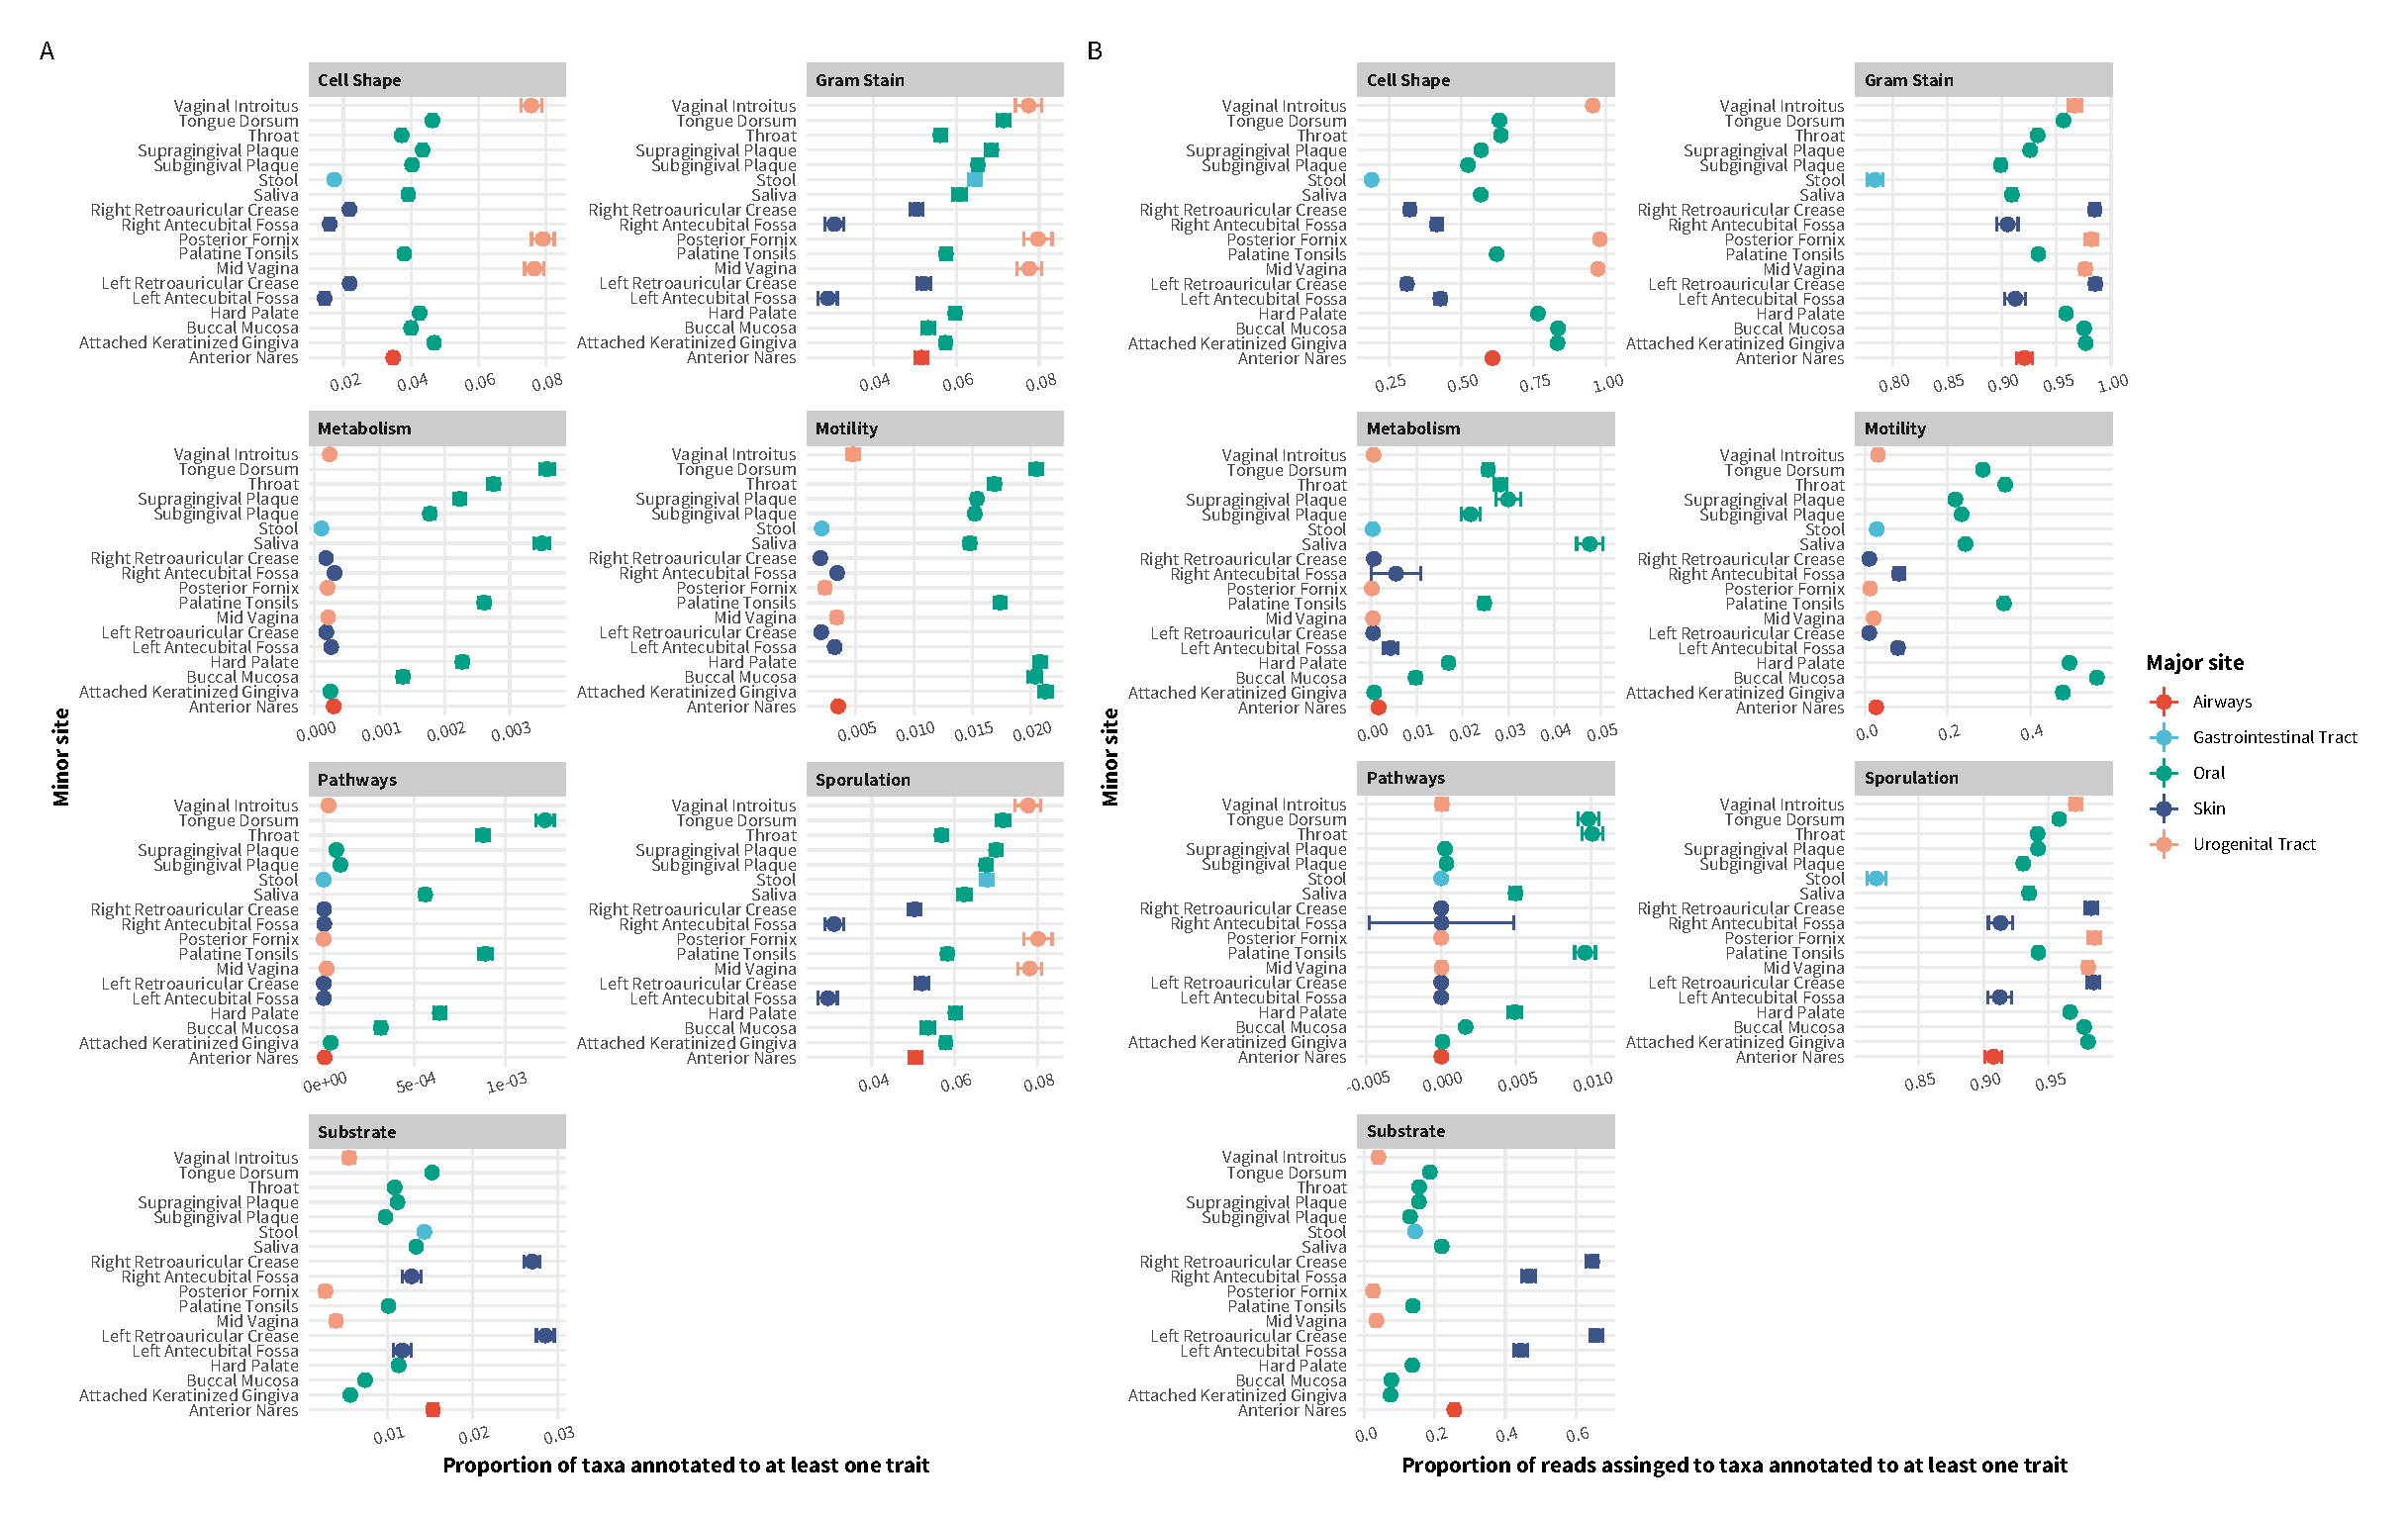
\includegraphics[width=\linewidth]{figures/appD_fs1.eps}
    \caption[Trait coverage statistics for samples profiled with 16S rRNA gene metabarcoding]{Trait coverage statistics for samples profiled with 16S rRNA gene metabarcoding. Panel \textbf{(A)} illustrates the proportion of present taxa per sample annotated to at least one trait. Panel \textbf{(B)} illustrates the proportion of reads assigned to taxa annotated to at least one trait which accounts for taxa relative abundances. Each plot facet represents different trait categories that were evaluated. Error bar represents the standard error of the evaluation statistic of interest across the the total number of samples evaluated per body site.}
    \label{fig:d1}
\end{sidewaysfigure}

\begin{figure} [!ht]
    \centering
    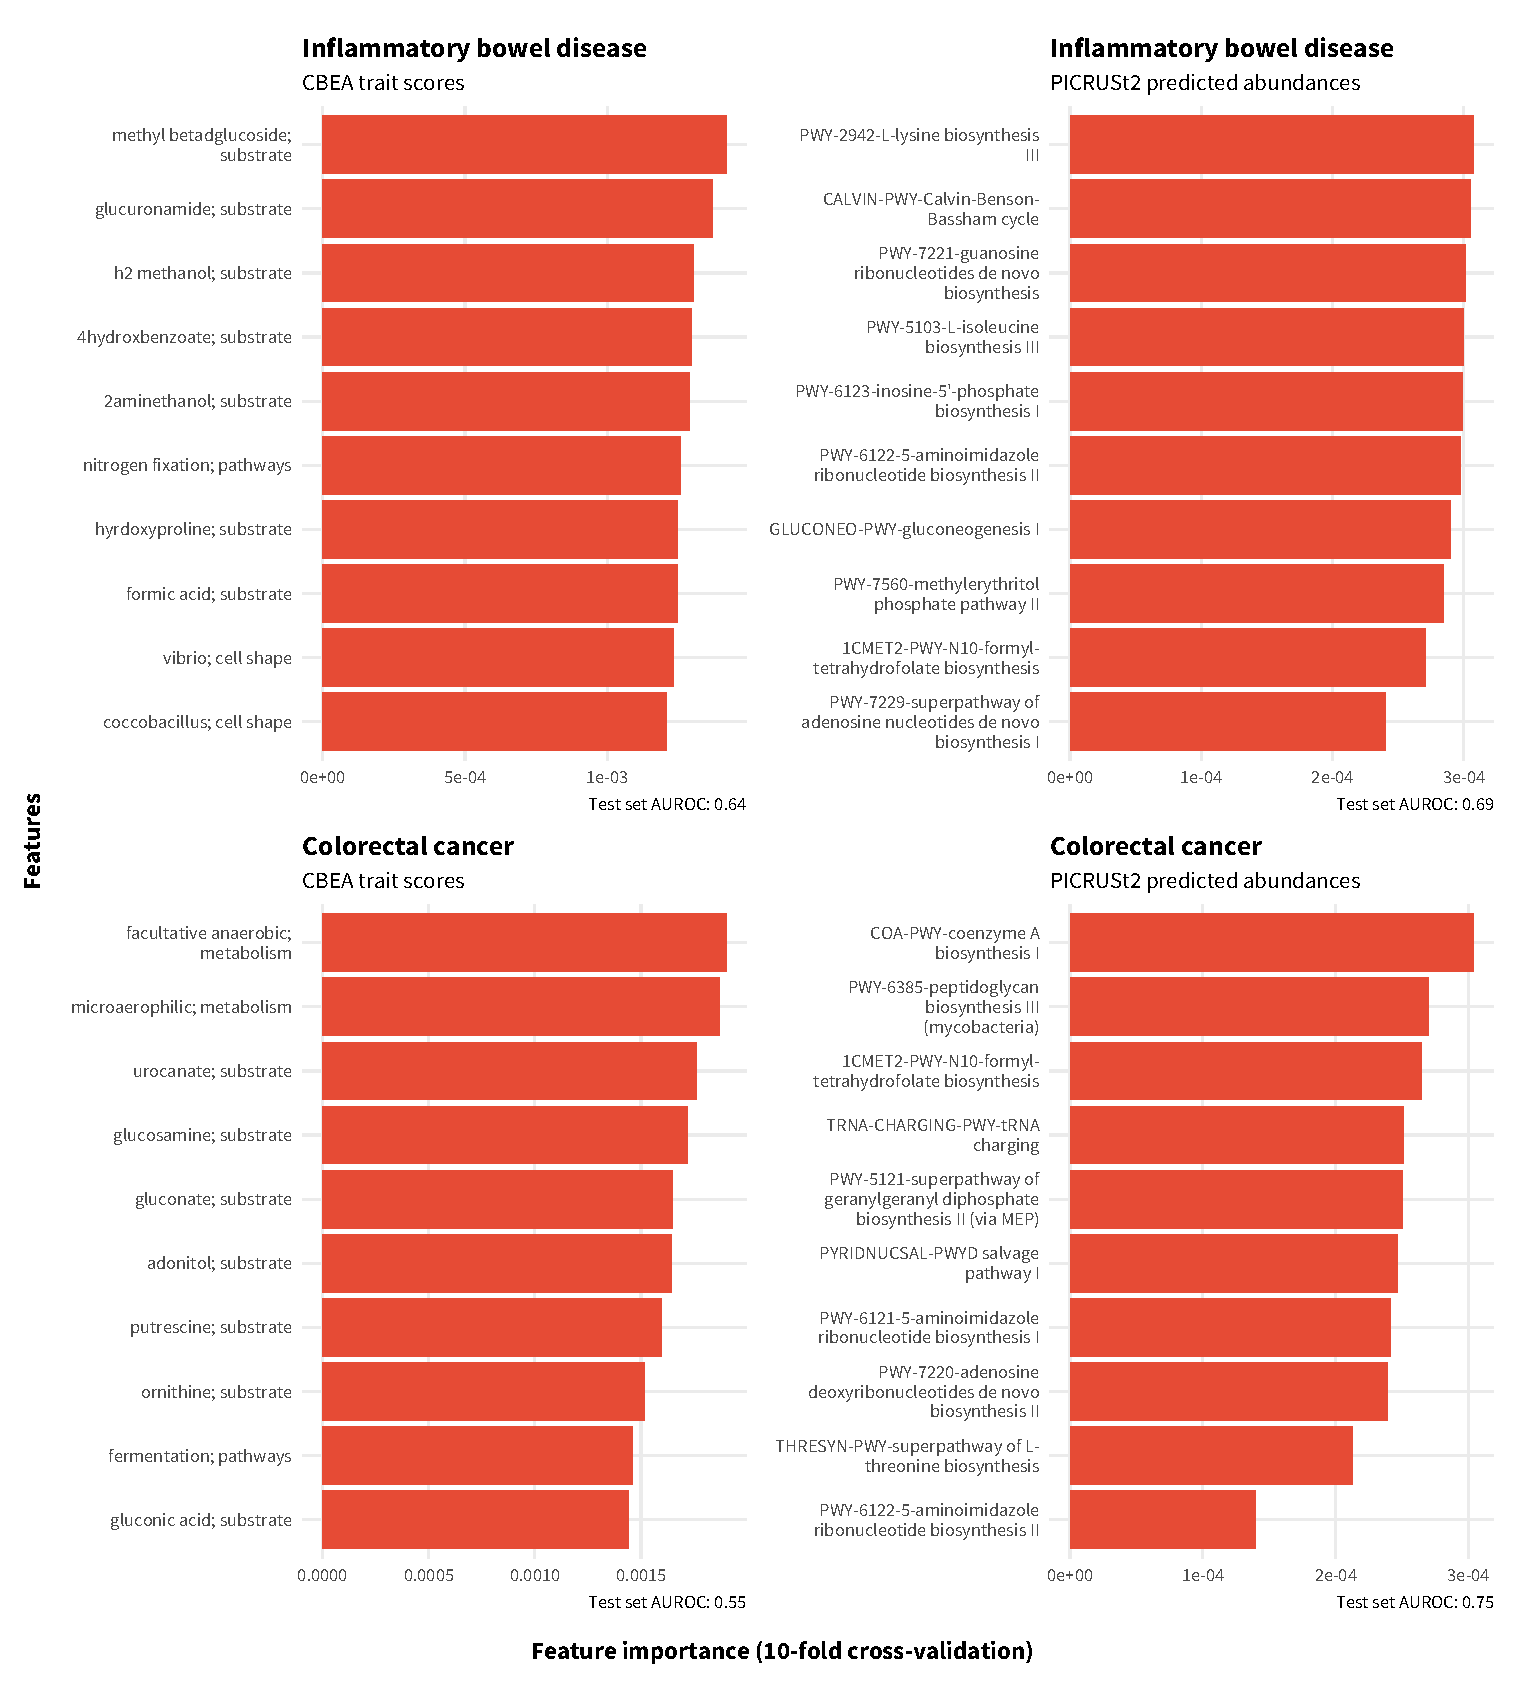
\includegraphics[width=\linewidth]{figures/appD_fs2.eps}
    \caption[Top 10 important features based on random forest model fitted different inputs from data sets profiled with 16S rRNA gene sequencing]{Top 10 important features based on random forest model fitted different inputs from data sets profiled with 16S rRNA gene sequencing. Features were selected from mean decrease in Gini impurity averaged across 500 decision trees and 10-fold cross-validation (nested with the training set) as implemented in \texttt{scikit-learn}. AUROC scored on a held-out test set is also presented for each input type and disease condition.}
    \label{fig:d2}
\end{figure}

%%%%%%%%%%%%%%%%%%%%%%%%%%%%%%%%%%%%%%%%%%%%%%%%%%
%Backend of thesis (references and the like)
%%%%%%%%%%%%%%%%%%%%%%%%%%%%%%%%%%%%%%%%%%%%%%%%%%
\backmatter

%Add your bibliography filename and uncomment these lines
\bibliographystyle{amsplain}
\addcontentsline{toc}{chapter}{References}
\bibliography{thesis}
\markboth{{\sffamily\sc Bibliography}}{}


%Uncomment if you want an index
%\printindex

\end{document}